% 150 câu đã gỡ khỏi ngân hàng (chuyen_dang) — chép lại vào file dạng để khôi phục

% từ: cau-hoi/lop10/0D2_BPT_va_he_BPT_bac_nhat_hai_an/0D2-2-2_Mien_nghiem_cua_He_BPT_bac_nhat_hai_an.tex
\begin{ex}%[0D2H2-2]%[ma:2aa162a8]
	Miền nghiệm (phần không tô màu) dưới đây biểu diễn tập nghiệm của hệ  bất phương trình nào?
	\begin{center}
		\begin{tikzpicture}[scale=1,font=\footnotesize,line join=round,line cap=round,>=stealth]
				\def\xmin{-3}\def\xmax{4}\def\ymin{-3}\def\ymax{3} 
				 \draw[->] (\xmin,0)--(\xmax,0) node[above]{$x$};
				\draw[->] (0,\ymin)--(0,\ymax) node[right]{$y$}; 
				\clip  (\xmin,\ymin) rectangle (\xmax,\ymax);
				\fill[pattern=north east lines] (\xmin,2) -- (\xmin,\ymin) -- (2,\ymin)--  cycle;
				\draw[smooth,samples=200,domain=\xmin:\xmax]  plot (\x,{(-1)*(\x)-1});
				\fill[pattern=north east lines] (\xmin,-4/3) -- (\xmin,\ymin)-- (\xmax,\ymin) -- (\xmax,1)--  cycle;
				 \draw[smooth,samples=200,domain=\xmin:\xmax] plot (\x,{(1/3)*(\x)-1/3});
				\foreach  \x in {-1,1}\draw (\x,-0.05)--(\x,0.05) node[above]{$\x$};
				\foreach \y in  {-1}\draw (-0.05,\y)--(0.05,\y) node[right]{$\y$};
				\fill (0,0) circle  (1pt) node[below left]{$O$};
			\end{tikzpicture}
	\end{center}
	 \def\dotEX{}
	 \choice
		{$\heva{&x-3y-1\ge 0\\&x+y+1> 0.}$} 
		{\True $\heva{&x-3y-1< 0  \\&x+y+1> 0.}$}
		{$\heva{&x-3y-1<  0\\&x+y+1\le 0.}$}
		{$\heva{&4x+3y-3< 0 \\&2x-y+2> 0.}$} 
	\loigiai{Trên đồ thị ta thấy $2$ đường thẳng  trên là $x-3y-1=0$ và $x+y+1=0$.\\
	Lại có điểm có tọa độ $O(0; 0)$ là điểm thuộc miền nghiệm. Thay tọa độ điểm $O(0; 0)$ vào đáp án ta  được $\heva{&0-3\cdot0-1< 0 \\&0+0+1> 0}$ nên miền nghiệm là của hệ bất phương trình $\heva{&x-3y-1< 0 \\&x+y+1> 0.}$}
\end{ex}

% từ: cau-hoi/lop10/0D3_Ham_so_bac_hai_va_do_thi/0D3-1-4_Do_thi_cua_ham_so.tex
\begin{ex}%[0D3B1-4]%[ma:025a6998]
	Cho hàm  số $y=2 x^2-x-3$, điểm nào sau đây thuộc đồ thị hàm số?
	 \choice
		 {$M(1; 0)$}
		 {$M(2; 7)$}
		 {\True $M(0;-3)$}
		 {$M(-1;-2)$}
	 \loigiai{
		Với $x=0$, ta có $y=2\cdot0^2-0-3=-3$. Suy ra đồ thị hàm số đi qua điểm $M(0;-3)$. 
	} 
\end{ex}

% từ: cau-hoi/lop10/0D3_Ham_so_bac_hai_va_do_thi/0D3-1-5_Tinh_dong_bien_nghich_bien.tex
\begin{ex}%[0D3N1-5]%[ma:74e1f31f]
	\immini[thm]{Cho hàm số $y=f(x)$ có tập xác định là $[-3;3]$ và đồ thị của nó được biểu diễn bởi hình bên. Khẳng định nào  sau đây đúng?
	\choice 
		{\True Hàm  số đồng biến trên khoảng $(-3;-1)$}
		{Hàm số đồng biến  trên khoảng $(-3;3)$}
		 {Hàm số đồng biến trên khoảng $(-3;0)$}
		{Hàm số nghịch biến trên  khoảng $(-1;2)$}}{
		\begin{tikzpicture}[>=stealth,x=1.0 cm,y=1.0 cm,scale=0.75]
				\draw[->] (-3.5,0)--(4,0)  node[below left] {$x$};
				\draw[->] (0,-2)--(0,4.5) node[below right] {$y$}; 
				\foreach \x in {,-3,-2,-1,1,2,3,,} 
				\draw[shift={(\x,0)},color=black]  (0pt,2pt) -- (0pt,-2pt) node[below] {\footnotesize $\x$};
				 \foreach \y in {,-1,1,2,3,4,}
				\draw[shift={(0,\y)},color=black]  (2pt,0pt) -- (-2pt,0pt) node[left] {\footnotesize $\y$};
				\draw[color=black]  (0pt,-10pt) node[right] {\footnotesize $0$};
				 \clip (-4,-2.5) rectangle (4,4.5);
				 \draw[dashed] (0,-1)--(-3,-1)--(-3,0);
				\draw[dashed]  (-1,0)--(-1,1)--(0,1);
				\draw[dashed] (0,4)--(3,4)--(3,0); 
				\draw[magenta,thick] (-3,-1)--(-1,1)--(0,1)--(3,4); 
			\end{tikzpicture}
		 }
	\loigiai{ 
		Trên khoảng $(-3;-1)$ và $(1;3)$, đồ thị hàm số đi lên, do đó hàm số đồng biến trên $(-3;-1)$ và $(1;3)$. 
	 }
\end{ex}

% từ: cau-hoi/lop10/0D3_Ham_so_bac_hai_va_do_thi/0D3-1-5_Tinh_dong_bien_nghich_bien.tex
\begin{bt}%[0D3H1-5]%[ma:e0c2f888]
	Cho hàm số $y=f(x)$ xác định trên đoạn $[-1;5]$ và có đồ thị như hình vẽ.
	\begin{center}\begin{tikzpicture}[>=stealth,x=1cm,y=1cm,scale=1]
			\draw[->](-1.8,0)--(-1,0)node[below]{$-1$}--(1,0)node[below]{$1$}--(2,0)node[below]{$2$}--(3,0)node[below]{$3$}--(4,0)node[above]{$4$}--(5,0)node[above]{$5$}--(5.8,0)node[above]{$x$};
			\draw[->] (0,-1.8)--(0,-1)node[left]{$-1$}--(0,1)node[right]{$1$}--(0,2)node[left]{$2$}--(0,3.2)node[right]{$y$};
			\draw (0,0)node[above left]{$O$};
			\fill[dashed] (-1,1)circle(2pt) edge (-1,0) edge (0,1) (2,2) circle edge (2,0) edge(0,2) (5,-1) circle edge (5,0) edge(0,-1) (-1,0)circle (1pt) (1,0)circle (1pt) (2,0)circle (1pt) (3,0)circle (1pt) (4,0)circle (1pt) (5,0)circle (1pt);
			\clip (-2,-2)rectangle(6,3.5);
			\draw[thick,samples=150,smooth] (-1,1)--(1,0)--(2,2);
			\draw[thick,samples=150,smooth]
			(2,2)..controls+(-20:1)and+(135:0.25)..(3.6,0)
			..controls+(-45:1)and+(155:1)..(5,-1)
			;
		\end{tikzpicture}
	\end{center}
	Hãy xác định các khoảng đồng biến, nghịch biến của hàm số $y=f(x)$ trên khoảng $(-1;5)$.
	\loigiai{
		Hàm số đồng biến trên $(1;2)$, hàm số nghịch biến trên các khoảng $(-1;1)$ và $(2;5)$.
	}
\end{bt}

% từ: cau-hoi/lop10/0D3_Ham_so_bac_hai_va_do_thi/0D3-1-5_Tinh_dong_bien_nghich_bien.tex
\begin{bt}%[0D3H1-5]%[ma:a061628a]
	Xét tính đồng biến, nghịch biến các hàm số sau:
	\begin{listEX}[1]
		\item $f(x)=x^2+2x-3$ trên khoảng $(-\infty;-1)$;
		\item $f(x)=2x+1$ trên khoảng $(1;+\infty)$.
	\end{listEX}
	\loigiai{
		\begin{listEX}[1]
			\item Ta xét: 
			\begin{eqnarray*}
				f(x_1)-f(x_2)&=&(x^2_1+2x_1-3)-(x^2_2+2x_2-3)\\&=& x^2_1-x^2_2+2(x_1-x_2)\\&=&(x_1-x_2)(x_1+x_2+2)
			\end{eqnarray*}
			$\forall x_1, x_2 \in (-\infty;-1)$ và $x_1<x_2$, ta có: $\heva{& x_1 < -1 \\ & x_2 < -1} \Rightarrow \dfrac{f(x_1)-f(x_2)}{x_1-x_2}=x_1+x_2+2<0$. \\
			Vậy hàm số nghịch biến trên $(-\infty;-1)$.
			\item Ta xét: 
			\begin{eqnarray*}
				f(x_1)-f(x_2)&=&(2x_1+1)-(2x_2+1)\\&=& 2(x_1-x_2)
			\end{eqnarray*}
			$\forall x_1, x_2 \in (1;+\infty)$ và $x_1 < x_2$, ta có: $\heva{& x_1 > 1 \\ & x_2 > 1} \Rightarrow \dfrac{f(x_1)-f(x_2)}{x_1-x_2}=2>0$. \\
			Vậy hàm số đồng biến trên $(1;+\infty)$.
		\end{listEX}
	}
\end{bt}

% từ: cau-hoi/lop10/0D3_Ham_so_bac_hai_va_do_thi/0D3-2-1_Xac_dinh_ham_so_bac_hai.tex
\begin{ex}%[0D3H2-1]%[ma:f918be39]
	Cho hàm  số $f(x)=-3x^2+x+2$. Các mệnh đề sau đúng hay sai?
	 \choiceTF
		 {Hàm số luôn nghịch biến trên $\mathbb{R}$}
		{\True Đồ thị hàm số đi qua điểm  $A(2;-8)$}
		{Hàm số đồng biến trên khoảng $(0;2)$} 
		{\True Giá trị lớn nhất của hàm số bằng $\dfrac{25}{12}$} 
	\loigiai{ 
		\begin{itemchoice}
			\itemch Hàm số bậc hai không thể đồng biến  hoặc nghịch biến trên $\mathbb{R}$ nên mệnh đề \lq\lq Hàm số luôn nghịch biến trên $\mathbb{R}$\rq\rq~sai.
			\itemch Vì $f(2)=-3\cdot 2^2+2+2=-8$ nên mệnh đề \lq\lq Đồ thị hàm số đi  qua điểm $A(2;-8)$\rq\rq~đúng.
			\itemch Hàm số $f(x)=-3x^2+x+2$ đồng biến trên khoảng $\left(-\infty;\dfrac{1}{6}\right)$ mà  $(0;2) \not\subset\left(-\infty;\dfrac{1}{6}\right)$.\\
			Vậy mệnh đề \lq\lq Hàm số đồng  biến trên khoảng $(0;2)$\rq\rq~sai.
			\itemch  Hàm số $f(x)=-3x^2+x+2$ đạt giá trị lớn nhất tại $x=\dfrac{1}{6}$ và $f\left(\dfrac{1}{6}\right)=-3\cdot \left(\dfrac{1}{6}\right)^2+\dfrac{1}{6}+2=\dfrac{25}{12}$ nên giá trị lớn nhất của hàm số bằng $\dfrac{25}{12}$.\\
			Vậy  mệnh đề \lq\lq Giá trị lớn nhất của hàm số bằng $\dfrac{25}{12}$\rq\rq~đúng.
		\end{itemchoice}
	} 
\end{ex}

% từ: cau-hoi/lop10/0D3_Ham_so_bac_hai_va_do_thi/0D3-2-3_Do_thi_cua_ham_so_bac_hai.tex
\begin{bt}%[0D3H2-3]%[Dự án Tex hóa toán 10 Cánh diều và Kết nối- GV10: Lê Văn Lý]%[ma:2c32e2fa]
	Vẽ đồ thị của mỗi hàm số sau:
	\begin{enumEX}[a)]{3}
		\item $y=x^2-3x-4$;
		\item $y=x^2+2x+1$;
		\item $y=-x^2+2x-2$.	
	\end{enumEX}
	\loigiai{
		\begin{enumEX}[a)]{1}
			\item \immini{Ta có $a=1, b=-3, c=-4, \Delta =(-3)^2-4\cdot 1\cdot(-4)=25.$
				\begin{itemize}
					\item Tọa độ đỉnh $I\left(\dfrac{3}{2};-\dfrac{25}{4}\right)$.
					\item Trục đối xứng $x=\dfrac{2}{3}$.
					\item Bảng giá trị
					\begin{center}
						\begin{tabular}{|c|c|c|c|c|c|}
							\hline
							$x$	&$-2$ &$-1$ &$0$ &$1$ \\
							\hline
							$y$	& $6$ & $0$ & $-4$ & $-6$ \\
							\hline
						\end{tabular}	
					\end{center}
				\end{itemize}
				Vẽ parabol đi qua các điểm được xác định ở trên, ta nhận được đồ thị hàm số $y=x^2-3x-4$.}{	
				\begin{tikzpicture}[>=stealth,x=1cm,y=1cm,scale=0.4]
					\def\a{1} % Hệ số a phải khác 0
					\def\b{-3}
					\def\c{-4}
					\draw[color=gray,dash pattern=on 1pt off 1pt,xstep=1.0cm,ystep=1.0cm] (-3,-7) grid (6,7);
					\draw[->] (-3,0) -- (6,0) node[below] {\scriptsize $x$};
					\draw[->] (0,-7) -- (0,7.1) node[left] {\scriptsize $y$};
					\draw[dashed] (0,0)node[above left]{\scriptsize $O$} (-1,0)node[below left]{\scriptsize $-1$} (0,-6)node[left]{\scriptsize $-6$}(1.5,0)node[above]{\scriptsize $\dfrac{3}{2}$}(0,6)node[above right]{\scriptsize $6$}--(-2,6)--(-2, 0)node[below left]{\scriptsize $-2$} (0, -6)--(1, -6)--(1, 0)node[above]{\scriptsize $1$};
					\pgfmathsetmacro\xdinh{-(\b)/2*(\a)}
					\pgfmathsetmacro\ydinh{(4*(\a)*(\c)-(\b)^2)/(4*(\a))}
					\fill[dashed] (\xdinh,\ydinh)circle(2pt) edge (\xdinh,0) edge (0,\ydinh);
					\clip (-3,-7)rectangle(6,7);
					\draw[thick,samples=150,smooth,domain=-4:6] plot(\x,{\a*(\x)^2+(\b)*\x+(\c)});
					\foreach \x/\y in{0/0, -1/0, -2/6, 0/-4, 1/-6 }
					\fill[black](\x,\y) circle (2pt);
			\end{tikzpicture}}
			\item 
			\immini{Ta có $a=1, b=2, c=1, \Delta =(2)^2-4\cdot 1\cdot 1=0$.
				\begin{itemize}
					\item Tọa độ đỉnh $I\left(-1;0\right)$.
					\item Trục đối xứng $x=-1$.
					\item Bảng giá trị
					\begin{center}
						\begin{tabular}{|c|c|c|c|c|c|}
							\hline
							$x$	&$-3$ &$-2$ &$-1$ &$0$ &$1$ \\
							\hline
							$y$	& $4$ & $1$ & $0$ & $1$ &$4$ \\
							\hline
						\end{tabular}	
					\end{center}
				\end{itemize}
				Vẽ parabol đi qua các điểm được xác định ở trên, ta nhận được đồ thị hàm số $y=x^2+2x+1$.}{	
				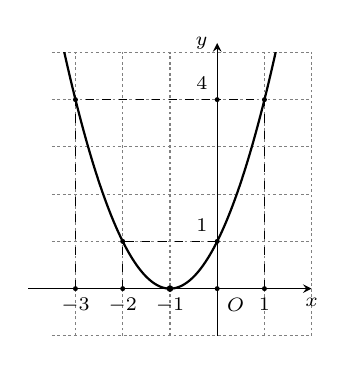
\begin{tikzpicture}[>=stealth,x=1cm,y=1cm,scale=0.6]
					\def\a{1} % Hệ số a phải khác 0
					\def\b{2}
					\def\c{1}
					\draw[color=gray,dash pattern=on 1pt off 1pt,xstep=1.0cm,ystep=1.0cm] (-3.5,-1) grid (2,5);
					\draw[->] (-4,0) -- (2,0) node[below] {\scriptsize $x$};
					\draw[->] (0,-1) -- (0,5.2) node[left] {\scriptsize $y$};
					\draw[dashed] (0,0)node[below right]{\scriptsize $O$} (-3, 0) node[below]{\scriptsize $-3$}--(-3,4)--(0, 4) node[above left]{\scriptsize $4$} (-2, 0) node[below]{\scriptsize $-2$}--(-2,1)--(0, 1) node[above left]{\scriptsize $1$} (-1, 0)node[below]{\scriptsize $-1$} (1, 0) node[below]{\scriptsize $1$}--(1,4)--(0, 4) ;
					\pgfmathsetmacro\xdinh{-(\b)/2*(\a)}
					\pgfmathsetmacro\ydinh{(4*(\a)*(\c)-(\b)^2)/(4*(\a))}
					\fill[dashed] (\xdinh,\ydinh)circle(2pt) edge (\xdinh,0) edge (0,\ydinh);
					\clip (-3.5,-1)rectangle(2,5);
					\draw[thick,samples=150,smooth,domain=-3.5:1.5] plot(\x,{\a*(\x)^2+(\b)*\x+(\c)});
					\foreach \x/\y in{0/0, -3/0, -3/4, -2/0, -2/1, 0/1, 1/0, 1/4, 0/4}
					\fill[black](\x,\y) circle (1.5pt);
			\end{tikzpicture}}
			\item 
			\immini{Ta có $a=-1, b=2, c=-2, \Delta =(2)^2-4\cdot (-1)\cdot (-2)=-4$.
				\begin{itemize}
					\item Tọa độ đỉnh $I\left(1;-1\right)$.
					\item Trục đối xứng $x=1$.
					\item Bảng giá trị
					\begin{center}
						\begin{tabular}{|c|c|c|c|c|c|}
							\hline
							$x$	&$-1$ &$0$ &$1$ &$2$ &$3$ \\
							\hline
							$y$	& $-5$ & $-2$ & $-1$ & $-2$ &$-5$ \\
							\hline
						\end{tabular}	
					\end{center}
				\end{itemize}
				Vẽ parabol đi qua các điểm được xác định ở trên, ta nhận được đồ thị hàm số $y=-x^2+2x-2$.}{	
				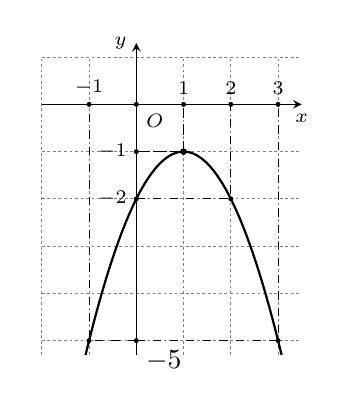
\begin{tikzpicture}[>=stealth,x=1cm,y=1cm,scale=0.6]
					\def\a{-1} % Hệ số a phải khác 0
					\def\b{2}
					\def\c{-2}
					\draw[color=gray,dash pattern=on 1pt off 1pt,xstep=1.0cm,ystep=1.0cm] (-2,-5.3) grid (3.5,1);
					\draw[->] (-2,0) -- (3.5,0) node[below] {\scriptsize $x$};
					\draw[->] (0,-5.3) -- (0,1.3) node[left] {\scriptsize $y$};
					\draw[dashed] (0,0)node[below right]{\scriptsize $O$} (0, -5)node[below right]{$\scriptsize -5$}--(-1, -5)--(-1, 0)node[above]{\scriptsize $-1$} (0, -1)node[left]{\scriptsize $-1$}--(1, -1)--(1, 0)node[above]{\scriptsize $1$} (0, -2)node[left]{\scriptsize $-2$}--(2, -2)--(2, 0)node[above]{\scriptsize $2$} (0, -5)--(3, -5)--(3, 0)node[above]{\scriptsize $3$};
					\pgfmathsetmacro\xdinh{-(\b)/2*(\a)}
					\pgfmathsetmacro\ydinh{(4*(\a)*(\c)-(\b)^2)/(4*(\a))}
					\fill[dashed] (\xdinh,\ydinh)circle(2pt) edge (\xdinh,0) edge (0,\ydinh);
					\clip (-2.3,-5.3)rectangle(3.3,1);
					\draw[thick,samples=150,smooth,domain=-2.3:3.3] plot(\x,{\a*(\x)^2+(\b)*\x+(\c)});
					\foreach \x/\y in{0/0,0/-5, 0/-2, -1/0, 2/0, 3/0, 3/-5, -1/-5, 0/-1, 2/-2, 1/0}
					\fill[black](\x,\y) circle (1.5pt);
			\end{tikzpicture}}
		\end{enumEX}
	}	
\end{bt}

% từ: cau-hoi/lop10/0D3_Ham_so_bac_hai_va_do_thi/0D3-2-6_Toan_thuc_te_ung_dung_ham_so_bac_hai.tex
\begin{ex}%[0D3H2-6]%[ma:14c4b0fd]
	 \immini[thm]{
	Một chiếc cổng hình parapol dạng $y=-x^2$ có chiều rộng $d=8$m. Hãy  tính chiều cao $h$ của cổng.
	\choice 
		{$h=9$m} 
		 {$h=8$m}
		{\True $h=16$m} 
		{$h=5$m} 
		}{ 
		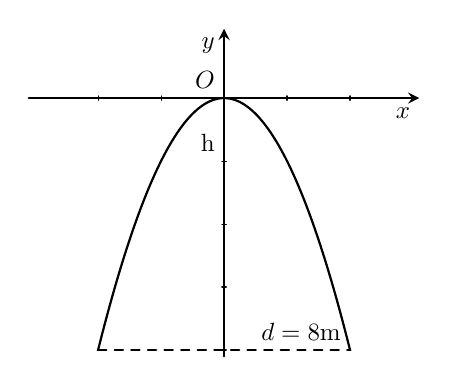
\begin{tikzpicture}[line join=round,line cap=round,>=stealth,thick,scale=0.8]
				\tikzset{every  node/.style={scale=0.9}}
				\draw[->]  (-3.1,0)--(3.1,0) node[below left] {$x$};
				\draw[->] (0,-4.1)--(0,1.1) node[below  left] {$y$};
				\draw[dashed] (-2,-4) --  (2,-4) node[above left] {$d=8$m};
				\draw (0,-1)  node[above left] {h};
				\draw (0,0)  node [above left] {$O$};
				\foreach  \x/\nx in {-2/-2,-1/-1,1/1,2/2}
				\draw[thin]  (\x,1pt)--(\x,-1pt);
				\foreach  \y/\ny in {-1/-1,-2/-2,-3/-3,-4/-4}
				\draw[thin] (1pt,\y)--(-1pt,\y); 
				\begin{scope}
					\clip (-3,-4) rectangle  (3,1);
					\draw[samples=200,domain=-3:3,smooth,variable=\x] plot  (\x,{-1*(\x)^2+0*(\x)+0});
				\end{scope}
			\end{tikzpicture}
		} 
	 \loigiai{
		Dựa vào hệ trục tọa độ hình minh họa $d=8$m suy ra đồ  thị hàm số đi qua điểm có tọa độ $(4; h)$ Suy ra $h=-4^2=-16$. Mà thực tế $h$ là chiều cao cổng nên $h=16$m.
	} 
\end{ex}

% từ: cau-hoi/lop10/0D7_Bat_phuong_trinh_bac_2_mot_an/0D7-2-7_Toan_thuc_te_ung_dung_bat_phuong_trinh_bac_2.tex
\begin{bt}%[0D7V2-7]%[Tex hóa SGK CD-CT,T7/22, Phạm Tiến Long]%[ma:43d3b643]
	Một hình chữ nhật có chu vi bằng $20$ cm. Để diện tích hình chữ nhật lớn hơn hoặc bằng $15\rm{ cm}^2$ thì chiều rộng của hình chữ nhật nằm trong khoảng bao nhiêu?
	\loigiai{
		Gọi $x$ (cm) là chiều rộng của hình chữ nhật. Khi đó chiều dài của hình chữ nhật là $10-x(\rm{cm})$\\
		Ta có $0<x \leq 10-x$, hay $0<x \leq 5$ (cm).\\
		Diện tích của hình chữ nhật là $S=x(10-x)$.\\
		Ta có $x(10-x) \geq 15$ khi và chỉ khi $-x^2+10x-15 \geq 0$, hay $x \leq -5-2\sqrt{10}$ hoặc $x \geq -5+2\sqrt{10}$.\\
		So với điều kiện (1), ta có $-5+2\sqrt{10} \leq x \leq 5$.\\
		Vậy chiều rộng của hình chữ nhật nằm trong khoảng từ $1{,}33$ cm đến $5$ cm.}
\end{bt}

% từ: cau-hoi/lop10/0D7_Bat_phuong_trinh_bac_2_mot_an/0D7-2-7_Toan_thuc_te_ung_dung_bat_phuong_trinh_bac_2.tex
\begin{bt}%[0D7V2-7]%[ma:e9d045b5]
	Một vật được ném theo phương thẳng đứng xuống dưới từ độ cao $320$ m với vận tốc ban đầu $v_0=20$ m/s. Hỏi sau ít nhất bao nhiêu giây, vật đó cách mặt đất không quá $100$ m? Biết rằng vật chuyển động nhaanh đàn đều và độ cao so với mặt đất của vật được mô tả bởi một hàm số bậc hai $h(t)=v_0t+\dfrac{1}{2}gt^2$, trong đó $v_0$ m/s là vận tốc ban đầu của vật, $t$ là thời gian chuyển động tính bằng giây, $g$ là gia tốc trọng trường (thường lấy $g \approx 10$ m/s$^2$) và độ cao $h(t)$ tính bằng mét và giả thiết rằng sức cản của không khí là không đáng kể (kết quả viết dưới dạng số thập phân và làm tròn đến hàng phần trăm).
	\shortans[]{$4{,}93$}
	\loigiai{
		Ta có $h(t)=20\cdot t+\dfrac{1}{1}\cdot 10\cdot t^2$ hay $h(t)=5t^2+20t$.\\
		Vật ném xuống từ độ cao $320$ m nên khi vật cách mặt đất không quá $100$ m có nghĩa là vật đã chuyển động được quãng đường lớn hơn hoặc bằng $320-100=220$ m.\\ 
		Khi đó $h(t)\ge 220$ hay $5t^2+20t\ge 220\Leftrightarrow t^2+4t-44\ge 0\quad (1)$.\\ 
		Tam thức $f(t)=t^2+4t-44$ có hai nghiệm $t_1=-2-4\sqrt 3$ và $t_2=-2+4\sqrt 3$.\\
		Mặt khác hệ số $a=1>0$ nên ta có bảng xét dấu
		\begin{center}
			
\begin{tikzpicture}
				\tkzTabInit[deltacl=0.5,espcl=2.5,lgt=2,nocadre]
				{$t$/1,$f(t)$/1}
				{$-\infty$,$-2-4\sqrt 3$,$-2+4\sqrt 3$,$+\infty$}
				\tkzTabLine{,+,0,-,0,+,}
			\end{tikzpicture}
		\end{center}
		Suy ra bất phương trình $(1)$ có nghiệm $t\le -2-4\sqrt 3$ hoặc $t\ge -2+4\sqrt 3$.\\ 
		Mà thời gian $t>0$ nên $t\ge -2+4\sqrt 3\approx 4{,}93$.\\
		Vậy sau ít nhất khoảng $4{,}93$ giây thì vật đó cách mặt đất không quá $100$\,m.
	}
\end{bt}

% từ: cau-hoi/lop10/0D7_Bat_phuong_trinh_bac_2_mot_an/0D7-3-6_Toan_hinh_toan_thuc_te_ung_dung_phuong_trinh.tex
\begin{bt}%[Dự án Bài Giảng 10-11 Nhóm Toán & LaTex, Nguyễn Anh Tuấn]%[0D7V3-6]%[ma:ebe6bb2a]
	\immini{
		Một người đứng ở điểm $A$ trên một bờ sông rộng $300$ m, chèo thuyền đến vị trí $D$, sau đó chạy bộ đến vị trí $B$ cách $C$ một khoảng $800$ m (hình vẽ). Vận tốc chèo thuyền là $6$ km/h, vận tốc chạy bộ là $10$ km/h và giả sử vận tốc dòng nước không đáng kể. Tính khoảng cách từ vị trí $C$ đến vị trí $D$, biết tổng thời gian người đó chèo thuyền và chạy bộ từ $A$ đến $B$ là $7{,}2$ phút.
	}{
		\begin{tikzpicture}[line cap=round, line join=round, font=\footnotesize, >=stealth, scale=0.5,rotate=90]
			\tikzset{label style/.style={font=\footnotesize}}
			\path (0,0) coordinate (A)
			(3,0) coordinate (C)
			(3,-8) coordinate (B)
			(3,-3.5) coordinate (D);
			\draw (D)--(A)--(C);
			\draw[shorten >=-0.5cm, shorten <=-0.5cm] (A)--($(A)-(C)+(B)$);
			\draw[shorten >=-0.5cm, shorten <=-0.5cm] (C)--(B);
			\draw[shorten >=-0.5cm, shorten <=-0.5cm] (A)--(C);
			\draw[shorten >=-0.5cm, shorten <=-0.5cm] (B)--($(A)-(C)+(B)$);
			\draw[<->] ($(A)+(0,0.4)$)--($(C)+(0,0.4)$) node[left, midway]{$300$ m};
			\draw[<->] ($(C)+(0.4,0)$)--($(B)+(0.4,0)$) node[above, midway]{$800$ m};
			\foreach\x/\y in {A/-135,B/-45,C/45,D/-150} \draw[fill=black] (\x) circle (2pt)+(\y:0.6) node{$\x$};
		\end{tikzpicture}	
		
	}
	\loigiai{
		Đặt $CD=x$ m, $x>0$. Ta có vận tốc của người đó khi trèo thuyền và chạy bộ lần lượt là $100$ m/phút và $\dfrac{500}{3}$ m/phút. Khi đó thời gian người đó chèo thuyền và chạy bộ lần lượt là $\dfrac{\sqrt{x^2+300^2}}{100}$ phút và $\dfrac{3\left(800-x\right)}{500}$ phút. Theo giả thiết, ta có phương trình
		\begin{align*}
			&\dfrac{\sqrt{x^2+300^2}}{100}+\dfrac{3\left(800-x\right)}{500}=7{,}2 \Rightarrow \sqrt{x^2+300^2}=240+\frac{3x}{5}\\
			\Rightarrow\ &x^2+300^2=\left(240+\frac{3x}{5}\right)^2\Rightarrow \frac{16x^2}{25}-288x+32400=0\Rightarrow x=225.
		\end{align*}
		Thử lại, ta được $CD=225$ m.
	}
\end{bt}

% từ: cau-hoi/lop10/0D7_Bat_phuong_trinh_bac_2_mot_an/0D7-3-6_Toan_hinh_toan_thuc_te_ung_dung_phuong_trinh.tex
\begin{ex}%[0D7H3-6]%[Đề toán 10 - GHKII - THPT Chuyên Lương Thế Vinh - Tỉnh Đồng Nai - NH 24-25]%[Hieu Hieu Minh Minh]%[ma:c1c063af]
	\immini{Hai con tàu đang ở tại vị trí $A$ (tàu $X$) và $B$ (tàu $Y$) cách nhau $10$ km cùng di chuyển về bến đỗ ở điểm $C$. Biết rằng hai tàu di chuyển theo đường thẳng cùng tốc độ $30$ km/h và phương di chuyển của hai tàu vuông góc với nhau (tham khảo hình vẽ). Tàu di chuyển từ $A$ đến $C$ trước tàu di chuyển từ $B$ trước 4 phút. Đặt $AC = x$ km.}{
		\begin{tikzpicture}[line join = round, line cap = round, scale=.8] 
			\coordinate[label = left:$C$] (C) at (0,0); 
			\coordinate[label = right:$B$] (B) at ($(C)+(2,0)$); 
			\coordinate[label = above:$A$] (A) at ($(C)+(0,3)$); 
			\draw[fill = gray!50] ($(C)!5pt!(B)$)--($(C)!5pt!(B)+(C)!5pt!(A)-(C)$)--($(C)!5pt!(A)$)--(C)--cycle;
			\draw (C)--(B)--(A)--cycle; 
			\foreach \x in {C,B,A} \fill[black] (\x) circle (1.5pt); 
		\end{tikzpicture} 
	}
	\choiceTF
	{\True Thời gian tàu $X$ đi từ $A$ đến $C$ bằng $\dfrac{x}{30}$ giờ}
	{$\dfrac{BC}{30} - \dfrac{x}{30} = 4$}
	{$BC = \sqrt{x^2 - 100}$}
	{\True Khoảng cách giữa $A$ và $C$ là $6$ km}
	\loigiai{
		Ta có $4$ phút $= \dfrac{4}{60}$ giờ $= \dfrac{1}{15}$ giờ.\\
		\begin{itemchoice}
			
			\itemch \textbf{Đúng}.\\
			Thời gian tàu $X$ đi từ $A$ đến $C$ là $\dfrac{x}{30}$ giờ.
			\itemch \textbf{Sai}.\\
			Thời gian tàu $Y$ đi từ $B$ đến $C$ là $\dfrac{BC}{30}$ giờ.\\
			Vì tàu $X$ đến $C$ trước tàu $Y$ $4$ phút nên $\dfrac{BC}{30} - \dfrac{x}{30} = \dfrac{1}{15}$ (*).
			\itemch \textbf{Sai}.\\
			Áp dụng định lý Pythagore trong tam giác $ABC$ vuông tại $C$ \\
			$$AB^2 = AC^2 + BC^2 \Rightarrow 10^2 = x^2 + BC^2 \Rightarrow 100 = x^2 + BC^2 \text{  (**)}$$
			Suy ra $BC = \sqrt{100 -x^2}$.
			\itemch \textbf{Đúng}.\\
			Từ bước (*), ta có $BC = x + 2$.\\
			Thay $BC = x + 2$ vào phương trình (**), ta được $100 = x^2 + (x+2)^2$.\\
			Giải phương trình
			\begin{eqnarray*}
				&& 100 = x^2 + x^2 + 4x + 4 \\
				&\Leftrightarrow& 2x^2 + 4x - 96 = 0 \\
				&\Leftrightarrow& x^2 + 2x - 48 = 0\\
				&\Leftrightarrow& \hoac{&x = 6\\&x = -8.}
			\end{eqnarray*} 
			Vì $x$ phải dương nên $x = 6$.\\
			Do đó khoảng cách từ $A$ đến $C$ là $6$ km.
		\end{itemchoice}
	}
\end{ex}

% từ: cau-hoi/lop10/0D8_Dai_so_to_hop/0D8-2-6_Bai_toan_co_yeu_to_hinh_hoc.tex
\begin{ex}%[0D8H2-6]%[ma:68ae002a]
	Trong  mặt phẳng cho một tập hợp gồm $6$ điểm phân biệt. Có bao nhiêu vectơ khác vectơ $\overrightarrow 0$ có điểm đầu và điểm cuối thuộc tập hợp điểm này?
	\choice 
		 {$15$}
		{$12$} 
		 {$1\,440$}
		 {\True $30$}
	\loigiai{ 
		Mỗi cặp sắp thứ tự gồm hai điểm $\left(A, B\right)$ cho ta một vectơ có điểm đầu $A$ và điểm cuối $B$ và ngược lại. Như vậy, mỗi vectơ có thể xem là một chỉnh hợp chập $2$ của tập hợp  $6$ điểm đã cho.\\
		Suy ra có $\mathrm{A}_6^2=30$  cách.
	} 
\end{ex}

% từ: cau-hoi/lop10/0D8_Dai_so_to_hop/0D8-2-6_Bai_toan_co_yeu_to_hinh_hoc.tex
\begin{bt}%[0D8H2-6]%[ma:8730da09]
	Trong mặt phẳng cho một  tập hợp gồm $6$ điểm phân biệt. Có bao nhiêu vectơ khác vectơ $\overrightarrow{0}$ có điểm đầu và điểm cuối thuộc tập hợp điểm này?
	\loigiai{ 
		Mỗi vectơ thỏa đề là một chỉnh hợp chập $2$ của $6$ nên  có $\mathrm{A}_6^2 = 30$ vectơ.
	 }
\end{bt}

% từ: cau-hoi/lop10/0D8_Dai_so_to_hop/0D8-2-6_Bai_toan_co_yeu_to_hinh_hoc.tex
\begin{bt}%[0D8H2-6]%[0D4K2]%[ma:1fa47b1f]
	Trong hình sau đây, mỗi cạnh của tam giác đều được chia thành $6$ đoạn thẳng bằng nhau bởi $5$ điểm nằm bên trong cùng với hai đầu mút. Hỏi có bao nhiêu tam giác có đỉnh là các chấm điểm ở trong hình?
	\begin{center}
		\begin{tikzpicture}
			\path
			(0:0) coordinate (A)
			(0:4) coordinate (B)
			($(A)!1!60:(B)$) coordinate (C)
			;
			\draw (A)--(B)--(C)--cycle;
			\foreach \x in {0,1,2,3,4,5,6}
			{
				\draw[fill=black] ($(A)!\x/6!(B)$) circle (1.5pt);
				\draw[fill=black] ($(B)!\x/6!(C)$) circle (1.5pt);
				\draw[fill=black] ($(C)!\x/6!(A)$) circle (1.5pt);
			}
		\end{tikzpicture}
	\end{center}
	\loigiai{
		Tổng số chấm điểm trong hình là $18$. Mỗi tam giác cần đếm được tạo ra bằng cách lấy ra $3$ điểm không thẳng hàng. Để đếm số các tam giác ta lấy số các cách lấy ra $3$ điểm từ $18$ điểm trừ đi số cách lấy ra $3$ điểm thẳng hàng từ $18$ điểm.\\
		Số các cách chọn $3$ điểm từ $18$ điểm là 
		$$\mathrm{C}^{3}_{18}=\dfrac{18!}{3!\cdot 15!}=816\;\text{(cách)}.$$
		Ba điểm thẳng hàng nếu chúng nằm trên cùng một cạnh. Số điểm của mỗi cạnh là $7$. Do đó, số cách lấy ra ba điểm trên mỗi cạnh là
		$$\mathrm{C}^{3}_{7}=\dfrac{7!}{3!\cdot 4!}=35\;\text{(cách)}.$$
		Như vậy, theo quy tắc cộng thì số các cách chọn ra $3$ điểm thẳng hàng từ $18$ điểm là
		$$35+35+35=105\;\text{(cách)}.$$
		Suy ra số các tam giác cần tìm là
		$$816-105=711\;\text{(tam giác)}.$$
	}
\end{bt}

% từ: cau-hoi/lop10/0H4_He_thuc_luong_trong_tam_giac/0H4-1-2_Tinh_cac_gia_tri_luong_giac.tex
\begin{bt}[Mức độ 1]%[Nguyễn Trung Kiên, dự án bài giảng 10-11, CTGDPT2018]%[0H4N1-2]%[ma:b3f1b774]
	Không dùng máy tính cầm tay, tính giá trị của biểu thức 
	$$A=\sin 0^\circ -\sin 55^\circ +\cos 60^\circ +\sin 125^\circ.$$
	\loigiai{ 
		Ta có $\sin 0^\circ=0$, $\cos 60^\circ=\dfrac{1}{2}$, $\sin 125^\circ = \sin\left(180^\circ - 55^\circ\right) = \sin 55^\circ$, suy ra
		$$A=0-\sin 55^\circ + \dfrac{1}{2} +\sin 55^\circ = \dfrac{1}{2}.$$ 
	}
\end{bt}

% từ: cau-hoi/lop10/0H4_He_thuc_luong_trong_tam_giac/0H4-1-2_Tinh_cac_gia_tri_luong_giac.tex
\begin{bt}%[0H4H1-2]%Nguyễn Thắng%[ma:41e7d3d4]
	Tính $\sin x$, $\cos x$, $\tan x$ và $\cot x$, biết
	\begin{listEX}[2]
		\item $\sin x+\cos x=\sqrt{2}$;
		\item $\sin x-\cos x=\sqrt{2}$.
	\end{listEX}
	\loigiai{
		\begin{listEX}
			\item Ta có 
			\begin{eqnarray*}
				\sin ^2x+\cos^2 x=1 &\Leftrightarrow& \left(\sqrt{2}-\cos x\right)^2+\cos^2x=1\\
				&\Leftrightarrow& 2\cos^2x-2\sqrt{2}\cos x +1=0\\
				&\Leftrightarrow& \cos x=\dfrac{\sqrt{2}}{2}.
			\end{eqnarray*}
			Suy ra $\sin x=\sqrt{2}-\cos x=\dfrac{\sqrt{2}}{2}$, $\tan x=\cot x=1$.
			\item Ta có 
			\begin{eqnarray*}
				\sin ^2x+\cos^2 x=1 &\Leftrightarrow& \left( \sqrt{2}+\cos x\right) ^2+\cos^2x=1\\
				&\Leftrightarrow& 2\cos^2x+2\sqrt{2}\cos x +1=0\\
				&\Leftrightarrow& \cos x=-\dfrac{\sqrt{2}}{2}.
			\end{eqnarray*}
			Suy ra $ \sin x=\sqrt{2}+\cos x=\dfrac{\sqrt{2}}{2} $, $ \tan x=\cot x=-1 $.
		\end{listEX}
	}
\end{bt}

% từ: cau-hoi/lop10/0H4_He_thuc_luong_trong_tam_giac/0H4-1-2_Tinh_cac_gia_tri_luong_giac.tex
\begin{bt}%[0H4N1-2]%[Dự án 4 - TLDH - TeamTeXHoa - Huỳnh Đức Vũ] %%[ma:82008ae9]
	Tính giá trị các biểu thức sau
	\begin{enumerate}
		\item  $A=a^2\sin{90^\circ}+b^2\cos{90^\circ}+c^2\cos{180^\circ}$.
		\item  $B=3-\sin^290^\circ+2\cos^260^\circ-3\tan^245^\circ$.
		\item  $C=\sin^245^\circ-2\sin^250^\circ+3\cos^245^\circ-2\sin^240^\circ+4\tan{55^\circ}\cdot \tan{35^\circ}$.
	\end{enumerate}
	\loigiai{
		\begin{enumerate}
			\item $A=a^2.1+b^2.0+c^2\cdot \left(-1\right)=a^2-c^2$.
			\item  $B=3-(1)^2+2\left(\dfrac{1}{2}\right)^2-3\left(\dfrac{\sqrt{2}}{2}\right)^2=1$.
			\item $C=\sin^245^\circ+3\cos^245^\circ-2\left(\sin^250^\circ+\sin^240^\circ\right)+4\tan{55^\circ}\cdot \cot{55^\circ}$.\\
			$C=\left(\dfrac{\sqrt{2}}{2}\right)^2+3\left(\dfrac{\sqrt{2}}{2}\right)^2-2\left(\sin^250^\circ+\cos^240^\circ\right)+4=\dfrac{1}{2}+\dfrac{3}{2}-2+4=4$.
	\end{enumerate}}
\end{bt}

% từ: cau-hoi/lop10/0H4_He_thuc_luong_trong_tam_giac/0H4-1-3_Bien_doi_rut_gon_bieu_thuc_luong_giac.tex
\begin{bt}[SGK CTST, Mức độ 2]%[BG - 10 New - 3in1, Nguyễn Văn Cường (Cường NV)]%[0H4H1-3]%[ma:cbf5b59f]
Cho tam giác $A B C$. Chứng minh rằng
\begin{listEX}[2]
\item  $\sin A=\sin (B+C)$.
\item $\cos A=-\cos (B+C)$.
\end{listEX}
\loigiai{
Trong $\triangle ABC$ ta có
\[\widehat{A} + \widehat{B} + \widehat{C} = 180^\circ \Rightarrow \widehat{A} = 180^\circ - (\widehat{B} + \widehat{C}).\]
\begin{listEX}[2]
\item Ta có
\[\sin A=  \sin (180^\circ - A) = \sin (B+C).\]
\item Ta có
\[\cos A = - \cos (180^\circ - A) = - \cos (B + C).\]
\end{listEX}}
\end{bt}

% từ: cau-hoi/lop10/0H4_He_thuc_luong_trong_tam_giac/0H4-1-3_Bien_doi_rut_gon_bieu_thuc_luong_giac.tex
\begin{bt}%[0H4H1-3]%[Dự án đề kiểm tra Toán 10 GHKI NH23-24 - Đỗ ĐƯờng Hiếu]%[THPT Võ Văn Kiệt- Tp HCM]%[ma:e5813fb7]
	Đơn giản các biểu thức $A=\sin 110^\circ-\sin 70^\circ+\cos 160^\circ+\cos 20^\circ-23\tan 12^\circ\cdot \cot 168^\circ+2000$.
	\loigiai{
		Ta có
		\begin{eqnarray*}
			A&=&\sin (180^\circ-70^\circ)-\sin 70^\circ+\cos (180^\circ-20^\circ)+\cos 20^\circ+\\
			&&-23\cdot \tan 12^\circ\cdot \cot(180^\circ-12^\circ)+2000\\
			&=&\sin 70^\circ-\sin 70^\circ-\cos20^\circ+\cos 20^\circ+23\cdot \tan 12^\circ\cdot \cot 12^\circ+2000=2023.	
		\end{eqnarray*}
	}
\end{bt}

% từ: cau-hoi/lop10/0H4_He_thuc_luong_trong_tam_giac/0H4-1-3_Bien_doi_rut_gon_bieu_thuc_luong_giac.tex
\begin{bt}%[0H4V1-3]%[ma:0074e448]
	
	Chứng minh rằng biểu thức sau đây không phụ thuộc vào $x$.
	\begin{enumEX}{2}
		\item  $A=\left( \sin x+\cos x \right)^2+\left( \sin x-\cos x \right)^2$.
		\item  $B=\sin^4 x-\cos^4 x-2\sin^2 x+1$.
	\end{enumEX}
	\loigiai{
		\begin{enumEX}{1}
			\item  $A=\left( \sin x+\cos x \right)^2+\left( \sin x-\cos x \right)^2=1+2\sin x\cos x+1-2\sin x\cos x=2$.\\
			\item  $\begin{aligned}[t]
				B&=\sin^4 x-\cos^4 x-2\sin^2 x+1=\left( \sin^2 x+\cos^2 x \right)\left( \sin^2 x-\cos^2 x \right)-2\sin^2 x+1\\
				&=1\left[ \sin^2 x-\left( 1-\sin^2 x \right) \right]-2\sin^2 x+1=0.
			\end{aligned}$
	\end{enumEX}}
\end{bt}

% từ: cau-hoi/lop10/0H4_He_thuc_luong_trong_tam_giac/0H4-2-1_Bai_toan_chi_dung_dinh_ly_Sin_Cosin.tex
\begin{bt}%[0H4V2-1] % KIEM_TRA%[Đào Trung Kiên]%[ma:2a1607fe]
	Cho tứ giác $ABCD$ có $AB \perp CD$; $AB=2$; $BC=13$; $CD=8$; $DA=5$ (hình bên dưới). Gọi $H$ là giao điểm của $AB$ và $CD$ và đặt $x=AH$. Hãy thiết lập một phương trình để tính độ dài $x$, từ đó tính diện tích tứ giác $ABCD$.
	\begin{center}
		\begin{tikzpicture}[thick,scale=1,nodes={scale=0.7}]
			\path 	(0:0) coordinate (C)
			++(0:-8) coordinate (D)
			++(0:-4) coordinate (H)
			++(-90:3) coordinate (A)
			++(-90:2) coordinate (B);
			\draw (A)--(B)--(C)--(D)--cycle;
			\draw (-12,-1.5)node[left]{$x$} (-10.3,-1.5)node[left]{$5$} (-12,-4)node[left]{$2$} (-5,0)node[above]{$8$} (-8,-4)node[above]{$13$};
			\draw[dashed](D)--(H)--(A);
			\path 	(0.3:0) coordinate (M)
			++(0:-0.3) coordinate (N)
			++(180:0.3) coordinate (P);
			\draw (-11.7,0)--(-11.7,-0.3)--(-12,-0.3);
			\draw (M)--(N)--(P);
			\foreach \x/ \goc in {A/180,B/-135,C/-45,D/45,H/180} 
			\fill (\x) circle (1pt)
			($(\x)+(\goc:3mm)$) node {$\x$};
		\end{tikzpicture}
	\end{center}	\loigiai{ 
		Đặt $x=HA$, $x\geq 0$.\\
		Vì $\triangle DHA$ vuông tại $H$ và $DA=5$ nên ta có $DH=\sqrt{25-x^2}$.\\
		Vì $\triangle CHB$ vuông tại $H$ nên theo định lý Pitago ta có 
		\begin{eqnarray*}
			BC^2=HC^2+HB^2&\Leftrightarrow& 13^2=\left(\sqrt{25-x^2}+8\right)^2+(2+x)^2	\\
			&\Leftrightarrow& 16\sqrt{25-x^2}=76-4x\\
			&\Leftrightarrow& 4\sqrt{25-x^2}=19-x\\
			&\Leftrightarrow& \heva{&19-x\geq 0\\&16(25-x^2)=(19-x)^2}\\
			&\Leftrightarrow& \heva{&x\leq 19\\&-17x^2+38x+39=0}\\
			&\Leftrightarrow& \heva{&x\leq 19\\&\hoac{&x=3\\&x=-\dfrac{13}{17}}}\\
			&\Leftrightarrow& x=3.
		\end{eqnarray*}
		Vậy $AH=3$, suy ra $HD=4$ nên diện tích $\triangle AHD$ là $S_{\triangle AHD}=\dfrac{1}{2}AH\cdot DH=6$.\\
		Diện tích $\triangle BHC$ là $S_{\triangle BHC}=\dfrac{1}{2}BH\cdot CH=30$.\\
		Từ đó suy ra diện tích tứ giác $ABCD$ bằng $S_{\triangle BHC}-S_{\triangle AHD}=30-6=24$ (đơn vị diện tích).
	}
\end{bt}

% từ: cau-hoi/lop10/0H4_He_thuc_luong_trong_tam_giac/0H4-2-2_Bai_toan_co_dung_cong_thuc_dien_tich.tex
\begin{bt}%[0H4N2-2]%[Tex hóa SGK CD-CT,T7/22, Phạm Tiến Long]%[ma:831b2924]
	\immini
	{
		Tính diện tích tam giác $ABC$ trong hình bên.
	}
	{
		\begin{tikzpicture}[scale=1, font=\footnotesize, line join=round, line cap=round, >=stealth]
			
			\path
			(0,3) coordinate (C)
			(4,1) coordinate (B)
			($(C)!2/3!-115:(B)$) coordinate (A)
			;
			\draw (A)--(C)node[pos=.5,rotate=41,above]{$8 $ cm}
			(B)--(C)node[pos=.5,rotate=-28,above]{$12 $ cm}
			(A)--(B) (0.3,2)node{$115^\circ$};
			\foreach \x/\g in {A/180,B/0,C/90} \fill[black] (\x) circle (1pt)+(\g:0.3) node{$\x$};
			\tkzMarkAngle[mark=,size =0.7](A,C,B)
		
\end{tikzpicture}
	}
	
	\loigiai{
		Diện tích tam giác $ABC$ là
		$$S=\dfrac{1}{2}ab\sin C=\dfrac{1}{2} \cdot 12 \cdot 8 \cdot \sin 115^\circ \approx 43{,}5\text{ cm}^2.$$}
\end{bt}

% từ: cau-hoi/lop10/0H4_He_thuc_luong_trong_tam_giac/0H4-3-1_Giai_tam_giac.tex
\begin{bt}[1,5 điểm]%[0H4H3-1]%[Dự án đề kiểm tra Toán 10 GKI NH24-25- Quan Ón]%[THPT Phạm Phú Thứ - Tp HCM] % KIEM_TRA%[ma:e1c519a1]
	Cho tam giác $MNP$ có $MN = 5$, $MP = P$ và $\widehat{M} = 60^\circ$.
	\begin{enumerate}
		\item Tính số đo góc $\widehat{N}$.
		\item Tính bán kính đường tròn nội tiếp tam giác $MNP$.
		\item Tính độ dài đường trung tuyến $NI$ của tam giác $MNP$.
	\end{enumerate}
	\loigiai{
		\begin{center}
			\begin{tikzpicture}[>=stealth,line join=round,line cap=round,font=\footnotesize,scale=1]
				\path 
				(0,0) coordinate (M)
				(5,0) coordinate (P)
				($(M) + (60:3.2)$) coordinate (N)
				($(M)!0.5!(P)$) coordinate (I)
				;
				\draw 
				(M)--(N)--(P)--(M) (N)--(I);
				;
				\foreach \p/\g in {M/-90, P/-90, N/90, I/-90}
				\draw[fill=black] (\p) circle (1pt) node[shift=(\g:3mm)] {$\p$};
				\pic[draw,angle radius=3mm,angle eccentricity=1.5] {angle = P--M--N};
				\fill (M) node[shift=(22:6.5mm)] {$60^\circ$};
				\path 
				(M) edge node[midway, sloped, rotate=50, anchor=center] {$ - $} (I)
				(I) edge node[midway, sloped, rotate=50, anchor=center] {$ - $} (P);
			\end{tikzpicture}
		\end{center}
		\begin{enumerate}
			\item Xét $\triangle MNP$, áp dụng định lí côsin, ta có
			\begin{eqnarray*}
				NP^2 &=& MN^2 + MP^2 - 2MN\cdot MP\cdot \cos\widehat{PMN}\\
				&=& 5^2 + 8^2 - 2\cdot 5\cdot 8\cdot\cos 60^\circ\\
				&=& 49\\
				\Rightarrow NP &=& \sqrt{49} = 7.
			\end{eqnarray*}
			Áp dụng hệ quả định lí côsin, ta có
			$$ \cos\widehat{MNP} = \dfrac{MN^2 + NP^2 - MP^2}{2\cdot MN\cdot NP} = \dfrac{5^2 + 7^2 - 8^2}{2\cdot 5\cdot 7} = \dfrac{1}{7} $$
			$\Rightarrow \widehat{MNP} \approx 81^\circ 47'$.
			\item Ta có $p = \dfrac{1}{2}(MN + NP + MP) = \dfrac{1}{2}(5 + 7 + 8) = 10$.\\
			Do đó $S_{\triangle MNP} = \dfrac{1}{2}MN\cdot MP\cdot\sin\widehat{MNP} = \dfrac{1}{2}\cdot 5\cdot 8\cdot\sin 60^\circ = 10\sqrt{3}$.\\
			Mà $S_{\triangle MNP} = pr \Rightarrow r = \dfrac{S_{\triangle MNP}}{p} = \dfrac{10\sqrt{3}}{10} = \sqrt{3}$.\\
			Vậy bán kính đường tròn nội tiếp tam giác $MNP$ bằng $\sqrt{3}$.
			\item Vì $NI$ là đường trung tuyến của $\triangle MNP$ nên $I$ là trung điểm của $MP$.\\
			Do đó $MI = \dfrac{1}{2}MP = \dfrac{1}{2}\cdot 8 = 4$.\\
			Xét $\triangle MNI$, áp dụng định lí côsin, ta có
			\begin{eqnarray*}
				NI^2 &=& MN^2 + MI^2 - 2\cdot MN\cdot MI\cdot\cos\widehat{NMI}\\
				&=& 5^2 + 4^2 - 2\cdot 5\cdot 4\cdot \cos 60^\circ\\
				&=& 21\\
				\Rightarrow NI &=& \sqrt{21}.
			\end{eqnarray*}
		\end{enumerate}
	}
\end{bt}

% từ: cau-hoi/lop10/0H4_He_thuc_luong_trong_tam_giac/0H4-3-2_Cac_ung_dung_thuc_te.tex
\begin{bt}%[0H4C3-2]%[ma:ff910aea]
	Một người muốn rào một mảnh vườn hình tam giác, trong đó một cạnh là bức tường có sẵn dài $6\text{ m}$, hai cạnh còn lại rào bằng lưới có tổng chiều dài $10\text{ m}$. Hỏi diện tích lớn nhất của mảnh vườn là bao nhiêu mét vuông?
	\shortans{12}
	\loigiai{
		Gọi hai cạnh rào là $b$, $c$ với $b+c=10$; nửa chu vi $p=\dfrac{6+10}{2}=8$.\\
		Theo công thức Heron: $S=\sqrt{8\cdot(8-6)(8-b)(8-c)}=\sqrt{16(8-b)(8-c)}$.\\
		Vì $(8-b)+(8-c)=6$ nên $(8-b)(8-c)\le\left(\dfrac{6}{2}\right)^2=9$.\\
		Suy ra $S\le\sqrt{16\cdot 9}=12$, dấu bằng khi $b=c=5$.\\
		Diện tích lớn nhất là $12\text{ m}^2$.
	}
\end{bt}

% từ: cau-hoi/lop10/0H5_Vecto_chua_xet_toa_do/0H5-2-6_Toan_thuc_te_ap_dung_tong_hieu_vecto.tex
\begin{ex}%[0H5H2-6]%[ma:ac9d4213]
	Một máy bay đang bay từ hướng Đông sang hướng Tây với tốc độ $650$ km/h thì gặp luồng gió thổi từ hướng Đông Bắc sang hướng Tây Nam  với vận tốc $35$ km/h. Máy bay bị thay đổi vận tốc sau khi gặp gió thổi.
	\begin{center}
		\begin{tikzpicture}[scale=1,font=\footnotesize,line join=round,line cap=round,>=stealth]
				\foreach  \a/\text in {0/Đông,45/Đông Bắc,90/Bắc,135/Tây Bắc,180/Tây,225/Tây Nam,270/Nam,315/Đông Nam}{
					\draw[->] (0,0)  -- (\a:1.8);
					\node at  (\a:2.4) {\text};}
			\end{tikzpicture}
			\begin{tikzpicture}[line cap=round,line join=round]
				\path[left color=cyan!80!black,right color=cyan!80!black] 
					(2.32,0.03).. controls (2.27,0.11) and (2.93,1.15).. 
					(3.21,1.64)..  controls (3.21,1.64) and (1.91,1.29)..
					(1.26,1.12).. controls (1.26,1.12)  and (1.55,1.43)..
					(1.34,1.62).. controls  (1.21,1.72) and (0.82,1.57)..
					(0.65,1.52).. controls (0.63,1.51)  and (0.01,2.28)..
					(0.01,2.31)..  controls (0.01,2.32) and (0.02,2.34)..
					(0.03,2.35).. controls (0.03,2.35)  and (0.47,2.5)..
					(0.56,2.47).. controls  (0.65,2.45) and (1.2,1.89)..
					(1.24,1.9).. controls  (1.26,1.9) and (4.22,2.69)..
					 (4.58,2.79).. controls (4.82,2.86) and (5.12,2.87)..
					(5.32,2.71).. controls (5.29,2.67) and  (4.86,2.63)..
					(4.86,2.52)..  controls (4.86,2.49) and (4.87,2.47)..
					(4.9,2.46).. controls  (5.07,2.44) and (5.53,2.61)..
					(5.53,2.61).. controls (5.7,2.65)  and (5.93,2.53)..
					(5.94,2.38).. controls (5.94,2.38) and  (4.25,1.92)..
					(4.24,1.92).. controls (4.24,1.91) and  (3.46,0.62)..
					(3.44,0.59).. controls  (3.18,0.25) and (2.38,-0.07).. cycle
					(2.02,2.65).. controls  (1.76,2.8) and (1.54,2.94)..
					(1.53,2.95).. controls (1.52,2.97) and  (1.52,2.98)..
					 (1.54,3).. controls (1.55,3.02) and (1.56,3.03)..
					(1.57,3.03).. controls (1.58,3.03) and  (1.71,3.05)..
					(1.86,3.07).. controls (2.01,3.09)  and (2.17,3.12)..
					(2.23,3.12).. controls (2.43,3.14) and (2.67,3.1).. 
					(2.84,3.01).. controls  (3.04,2.91) and (3.5,2.65)..
					(3.48,2.65).. controls (3.47,2.64) and (3.24,2.58).. 
					(2.98,2.51) -- (2.49,2.38)  -- cycle
					(4.4,1.81).. controls  (4.53,1.86) and (5.93,2.22)..
					 (5.97,2.23).. controls (5.99,2.24) and (5.99,2.24)..
					(5.98,2.21).. controls (5.92,1.79) and (4.81,1.61).. 
					(4.15,1.47).. controls (4.12,1.46)  and (4.33,1.79)..
					(4.4,1.81) -- cycle 
					 (1.45,1.02).. controls (1.83,1.13) and (2.87,1.4)..
					 (2.91,1.41).. controls (2.86,1.3) and (2.81,1.19)..
					(2.74,1.1)..  controls (2.32,1.02) and (1.88,0.97)..
					 (1.45,1.02) -- cycle
					(0.5,0.64).. controls (0.49,0.65) and (0.48,0.68).. 
					(0.48,0.69).. controls (0.56,0.91) and (0.64,1.16).. 
					(0.73,1.39).. controls (0.89,1.44) and  (1.04,1.48)..
					(1.21,1.52).. controls (1.26,1.53)  and (1.28,1.49)..
					(1.27,1.45).. controls (1.25,1.4) and (0.93,0.85).. 
					(0.89,0.8).. controls (0.82,0.69) and  (0.54,0.62).. cycle;
				\path (2.2,1.8)  coordinate (ta)
					(4.3,2.4) coordinate  (tb);
				 \foreach \x in {0,1,...,5}{
					 \pgfmathsetmacro{\vt}{\x/5}
					\fill[white]  ($(ta)!\vt!(tb)$) circle (0.08);
				} 
			\end{tikzpicture}
	\end{center}
	Tìm tốc độ mới của máy  bay (kết quả làm tròn đến hàng đơn vị, đơn vị: km/h).
	\choice 
		{\True $675$} 
		 {$674$}
		{$673$} 
		 {$676$}
	 \loigiai{Dựng hình bình hành $MNPQ$ thỏa mãn $\left|\overrightarrow{MN}\right|=650, \left|\overrightarrow{MQ}\right|=35$.\\
	\begin{center}
		\begin{tikzpicture}[scale=1,font=\footnotesize,line join=round,line cap=round,>=stealth]
				\coordinate  (M) at (13.3,0);
				\coordinate (N) at (6.8,0); 
				 \coordinate (Q) at (11.8,-1.5);
				\coordinate (P)  at (5.3,-1.5);
				\draw[dashed,->]  (M) -- (N)
					(M)--(Q); 
				 \draw[dashed] (N)--(P)--(Q);
				\draw[->,blue]  (M)--(P);
				\foreach  \x/\y in {M/90,N/90,P/-90,Q/-90} \fill[black](\x) circle (1pt)
					 ($(\x)+(\y:3mm)$) node{$\x$};
			\end{tikzpicture}
	\end{center}
	 Khi đó hướng bay và vận tốc mới của máy bay chính là vectơ $\overrightarrow{MP}$.\\
	Theo định lý cosintrong  tam giác $MNP$, ta có
	\[MP=\sqrt{MN^2+MQ^2-2\cdot MN\cdot MQ\cdot \cos  135^\circ}=\sqrt{423725+22750\sqrt{2}}\approx 675.\]
	 Tốc độ mới của máy bay là $675$ km/h.
	} 
\end{ex}

% từ: cau-hoi/lop10/0H9_Phuong_phap_toa_do_trong_mat_phang/0H9-3-2_Phuong_trinh_duong_thang.tex
\begin{bt}%[0H9H3-2]%[ma:01acb6ab]
	Quan sát \textit{Hình 64} và thực hiện các hoạt động sau:
	\begin{enumerate}[a)]
	\item Lập phương trình đường thẳng $d$;
	\item Lập phương trình đường tròn $(C)$;
	\item Lập phương trình tiếp tuyến của đường tròn $(C)$ tại điểm $M(2+\sqrt{2} ; 1+\sqrt{2})$.
	\end{enumerate}
	\[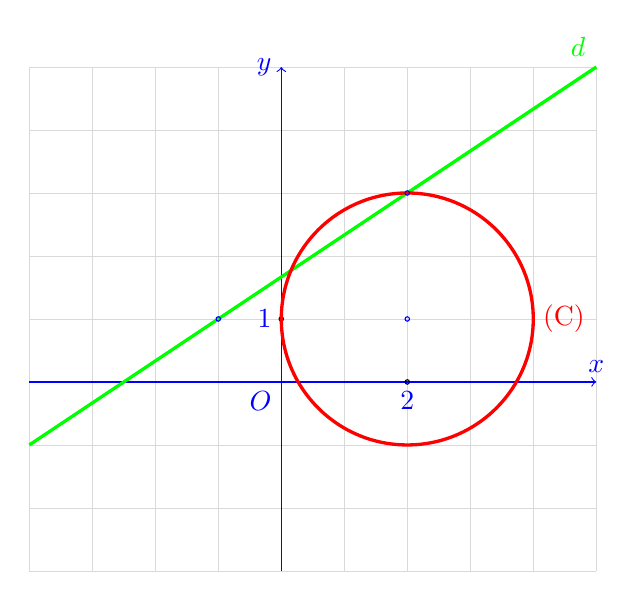
\begin{tikzpicture}[scale=0.8]
		\draw[step=1,gray, very thin,opacity=0.3](-4,-3) grid (5,5);
		\draw [->,blue] (-4,0) -- (5,0) node[above] {$x$};
		\draw [->,blue] (0,-3) -- (0,5) node[left] {$y$};
		\foreach \x in {2} {\draw (\x,0) node[below,blue] {$\x$} circle (1pt);}
		\foreach \y in {1} {\draw (0,\y) node[left,blue] {$\y$} circle (1pt);}
		\draw (0,0) node [below left,blue]{$O$};
		\draw[smooth,green, very thick] plot[domain=-4:5] (\x, {(2/3)*(\x) +(5/3)}) node[above left] {$d$};
		\draw[red, very thick] (2,1) circle (2) ;
		\draw (4,1) node [right,red] {(C)} ;
		\draw[blue] (-1,1) circle (1pt);
		\draw[blue] (2,3) circle (1pt);
		\draw[blue] (2,1) circle (1pt);
		\end{tikzpicture}\]
\loigiai{
	\begin{enumerate}[a)]
		\item Lập phương trình đường thẳng $d$;\\
		Dựa vào đồ thị hình 64, ta thấy đường thẳng $d$ đi qua hai điểm $A(-1;1)$ và $B(2;3)$.\\
		Phương trình tham số đường thẳng $d$ đi qua $A(-1;1)$ và có một vectơ chỉ phương là $\overrightarrow{u}=\overrightarrow{AB}=(3;2)$:\\
		\[d:\left\{ {\begin{array}{*{20}{c}}
		  {x =  - 1 + 3t} \\ 
		  {y = 1 + 2t} 
		\end{array}} \right.\]
		$(t \in \mathbb{R})$.
		\item Lập phương trình đường tròn $(C)$;\\
		Phương trình đường tròn $(C)$ có tâm $I(2;1)$ và bán kính $R=2$:
				\[(C): (x-2)^2+(y-1)^2=4\]
		\item Lập phương trình tiếp tuyến của đường tròn $(C)$ tại điểm $M(2+\sqrt{2} ; 1+\sqrt{2})$.\\
		Gọi $d$ là tiếp tuyến của đường tròn $(C)$ tại điểm $M$. \\
		Khi đó $d$ và $IM$ vuông góc với nhau.\\
		Phương trình đường thẳng $d$ qua $M(2+\sqrt{2} ; 1+\sqrt{2})$ và $\overrightarrow{IM}=(\sqrt{2} ; \sqrt{2})$ là vectơ pháp tuyến:\\
		\[d: \sqrt{2}(x-2-\sqrt{2})+\sqrt{2}(y-1-\sqrt{2})=0\]
		\[d: (x-2-\sqrt{2})+(y-1-\sqrt{2})=0\]
		\[d: x+y-3-2\sqrt{2})=0\]
		\end{enumerate}
}
\end{bt}

% từ: cau-hoi/lop10/0H9_Phuong_phap_toa_do_trong_mat_phang/0H9-3-6_Bai_toan_tim_diem.tex
\begin{bt}%[0H9H3-6]%[ma:b0d34620]
	Trong mặt phẳng  toạ độ $Oxy$, cho hình bình hành $ABCD$ có diện tích bằng $2$. Biết $A(0;2),B(3;0)$ và giao điểm $I$ của hai đường chéo hình bình hành nằm trên đường thẳng $y=-x$. Tìm hoành độ đỉnh $D$, biết $x_D>-14$.
	\loigiai{ 
		Phương trình đường thẳng $AB$ là $\dfrac{x}{3}+\dfrac{y}{2}=1\Leftrightarrow  2x+3y-6=0$.\\
		Điểm $I$ nằm trên đường thẳng $y=-x$ nên giả  sử $I(t;-t)$.\\
		 Vì $I$ là trung điểm của $AC$ nên $C(2t;-2t-2),I$ là trung điểm của $BD$ nên $D(2t-3;-2t)$.\\
		Ta có  $AB=\sqrt{(3-0)^2+(0-2)^2}=\sqrt{13}$.\\
		Suy ra  $\mathrm{d}(C,AB)=\dfrac{2}{\sqrt{13}}$.\\
		Khi đó $\dfrac{|2\cdot 2t+3(-2t-2)-6|}{\sqrt{2^2+3^2}}=\dfrac{2}{\sqrt{13}} \Leftrightarrow|-2t-12|=2$.\\ 
		Suy ra  $t=-5$ hoặc $t=-7$.
		\begin{itemize}
			\item Với $t=-5$, ta có  $C(-10;8),D(-13;10)$ nhận vì $x_D=-13>-14$.
			\item Với $t=-7$, ta có $C(-14;12),D(-17;14)$ loại  vì $x_D=-17<-14$.
		\end{itemize}
	} 
\end{bt}

% từ: cau-hoi/lop10/0H9_Phuong_phap_toa_do_trong_mat_phang/0H9-4-7_Bai_toan_thuc_te_PP_toa_do_hoa.tex
\begin{bt}%[0H9V4-7]%[ma:3a647451]
	\immini[thm]{ 
	Hình vẽ bên mô phỏng một trạm  thu phát sóng điện thoại di động đặt ở vị trí $I$ có tọa độ $(-2;1)$ trong mặt phẳng toạ độ (đơn vị trên hai trục là ki-lô-mét). Tính theo đường chim bay, xác định khoảng cách ngắn nhất để một người ở vị trí có toạ độ $(-3;4)$ di chuyển được tới vùng phủ sóng theo đơn vị ki-lô-mét (làm tròn kết quả đến hàng phần trăm). Biết rằng trạm thu phát sóng đó được thiết kế với bán kính phủ sóng $3$ (km).
	 }{
	\begin{tikzpicture}[line join=round,line cap=round,thick,scale= 0.6]
			\path 
				(0,0)  coordinate (O)
				(-2,1) coordinate (I)++(0:3) coordinate  (t);
			\draw[->] (-6,0)--(3,0)  node[below]{$x$};
			 \draw[->] (0,-3)--(0,6) node[right]{$y$};
			\draw[dashed] (-2,0) circle  (1pt) node[below]{$-2$} -- (-2,1) --(0,1) circle (1pt) node[right]{$1$};
			\draw [blue]let \p1 = ($(I) - (t)$) in  (I) circle ({veclen (\x1,\y1)});
			\foreach  \i/\g in {
				 O/-135,I/150
				}{\draw[fill=black](\i)  circle (1pt)
				($(\i)+(\g:4mm)$) node[scale=0.8]{$\i$};} 
		\end{tikzpicture}
	 }
	 \loigiai{
	 \immini{
		Đường tròn màu xanh mô tả ranh giới bên ngoài của vùng phủ sóng có tâm $I(-2;1)$ và bán kính phủ sóng $3$(km) nên phương  trình đường tròn đó là $(x+2)^2+(y-1)^2=9$.\\
		Giả sử vị  trí đứng của người đó là $B(-3;4)$.\\
		Gọi $A$ là  giao điểm thứ nhất của đường tròn tâm $I$ và $BI$.\\
		Suy ra khoảng cách ngắn  nhất để người đó di chuyển được từ vị trí $B(-3;4)$ tới vùng phủ sóng là $BA$.\\
		Ta  có $IB=\sqrt{(-3+2)^2+(4-1)^2}=\sqrt{10}$, suy ra $AB=IB-IA=\sqrt{10}-3\approx 0{,}16$.
		 }{
		\begin{tikzpicture}[line join=round,line cap=round,thick,scale= 0.8]
				\path 
					(0,0) coordinate  (O)
					 (-2,1) coordinate (I)++(0:3) coordinate (t);
				\draw (I)--(-3,4); 
				\draw[->]  (-6,0)--(3,0) node[below]{$x$};
				 \draw[->] (0,-3)--(0,6) node[right]{$y$};
				\draw (-3,4)  node[below right]{$A$};
				\draw[dashed] (-2,0) circle (1pt) node[below]{$-2$} --  (-2,1) --(0,1) circle (1pt) node[right]{$1$};
				\draw[dashed] (-3,0) circle (1pt) node[below]{$-3$} -- (-3,4) circle (1pt) node[above right]{$B$} --(0,4) circle  (1pt) node[right]{$4$};
				\draw [blue]let \p1 = ($(I) - (t)$) in (I) circle ({veclen (\x1,\y1)}); 
				\foreach \i/\g in { 
					 O/-135,I/180
					}{\draw[fill=black](\i) circle  (1pt)
					($(\i)+(\g:3mm)$)  node[scale=0.7]{$\i$};}
			\end{tikzpicture}
		 }
	} 
\end{bt}

% từ: cau-hoi/lop10/0H9_Phuong_phap_toa_do_trong_mat_phang/0H9-5-0_Bai_toan_tong_hop_thuc_te_PP_toa_do_hoa_3_duo.tex
\begin{bt}%[0H9V5-0]%[ma:ad167802]
	Để chụp toàn cảnh, ta có thể sử dụng một gương hypebol. Máy ảnh được hướng về phía đỉnh của gương và tâm quang học của  máy ảnh được đặt tại một tiêu điểm của gương (xem hình). Tìm khoảng cách từ tâm quang của máy ảnh đến đỉnh của gương, biết rằng phương trình mặt cắt của gương là $\dfrac{x^2}{25}-\dfrac{y^2}{16}=1$.
	\begin{center}
		\begin{tikzpicture}[scale=0.6,font=\footnotesize,line join=round,line cap=round,>=stealth]
				\def\xmin{-10}\def\xmax{10}\def\ymin{-5}\def\ymax{5}\pgfmathsetmacro\c{2*sqrt  (5)}
				\draw[->] (\xmin-0.2,0)--(\xmax+0.2,0) node[below] {\footnotesize $x$}; 
				 \draw[->] (0,\ymin-0.2)--(0,\ymax+0.2) node[right] {$y$};
				\clip (\xmin,\ymin) rectangle (\xmax,\ymax); 
				 \path
					 (0,0) coordinate (O)
					(-2,0)  coordinate (A_1)
					(2,0) coordinate  (A_2)
					 (-\c,0) coordinate (F_1)
					(\c,0) coordinate (F_2) 
					 (-6.3,3) coordinate (M)
					(-6.3,-3) coordinate  (N);
				 \draw[blue] (M)--(N);
				\fill[blue!50]  (F_2) circle (0.3cm);
				\fill[blue!10]  (M)--(N)--plot ({-2*sqrt (\x*\x+1)},{\x})--(M);
				 \draw[smooth,variable=\x,blue] plot ({2*sqrt (\x*\x+1)},{\x});
				 \draw[smooth,variable=\x,blue] plot ({-2*sqrt (\x*\x+1)},{\x});
				\foreach \x/\g  in {F_1/-90,F_2/-90}
				\fill  (\x) circle (4.5pt);
				\foreach \x/\g  in {F_1/-90,F_2/-90,A_1/-40,A_2/240,O/-120}
				 \fill (\x) circle (1.5pt)
					 ($(\x)+(\g:7mm)$) node{$\x$};
				\draw (M)--($(M)+(30:1)$) node[above]{gương hypebol}; 
				\draw (F_2)--($(F_2)+(130:3)$) node[above]{tâm máy  ảnh};
				 \draw[dashed](A_1)--(F_1);
			\end{tikzpicture}
	\end{center}
	\loigiai{ Gọi $(H)\colon \dfrac{x^2}{25}-\dfrac{y^2}{16}=1\Rightarrow  \heva{&a^2=25\\&b^2=16}\Rightarrow \heva{&a=5\\&b=4}\Rightarrow c=\sqrt{a^2+b^2}=\sqrt{39}$.\\
		Tiêu điểm của  gương là $F_1\left(-\sqrt{39};0\right)$ và $F_2\left(\sqrt{39};0\right)$.\\
		Đỉnh của gương là  $A_1(-5;0)$.\\
		Vậy khoảng cách từ tâm của máy ảnh tới đỉnh của gương là\\  $F_2A_1=OA_1+OF_2=5+\sqrt{39}\approx 11{,}2$.
	} 
\end{bt}

% từ: cau-hoi/lop11/1D1_Ham_so_luong_giac_va_phuong_trinh_luong/1D1-1-2_Chuyen_doi_don_vi_do_va_radian.tex
\begin{ex}[c]%[1D1B1-2]%[ma:b9cf1ffb]
	 Với $x\in \left(\dfrac{31\pi}{4};\dfrac{33\pi}{4}\right)$, mệnh đề nào sau đây là đúng?
	\choice 
		{Hàm số $y=\cot x$  nghịch biến}
		{\True Hàm số  $y=\sin x$ đồng biến}
		{Hàm số $y=\cos x$ nghịch  biến}
		{Hàm số $y=\tan  x$ nghịch biến}
	\loigiai{ 
	Ta có $\left(\dfrac{31\pi}{4};\dfrac{33\pi}{4}\right)=\left(-\dfrac{\pi}{4}+8\pi;\dfrac{\pi}{4}+8\pi \right)$ thuộc góc phần tư thứ  I và II.}
\end{ex}

% từ: cau-hoi/lop11/1D1_Ham_so_luong_giac_va_phuong_trinh_luong/1D1-1-2_Chuyen_doi_don_vi_do_va_radian.tex
\begin{ex}%[1D1B1-2]%[ma:4807c63e]
	Hàm số $y=\tan  x$ đồng biến trên khoảng nào sau đây?
	\choice{\True  $\left(0;\dfrac{\pi}{2}\right)$}{$(0;\pi)$}{$\left(\dfrac{\pi}{2};2 \pi\right)$}{$\left(\dfrac{\pi}{2};\dfrac{5 \pi}{2}\right)$}
	\loigiai{ 
		Hàm số $y=\tan x$ luôn đồng biến trên các khoảng xác định, vậy nó  đồng biến trên khoảng $\left(0;\dfrac{\pi}{2}\right)$.
	} 
\end{ex}

% từ: cau-hoi/lop11/1D1_Ham_so_luong_giac_va_phuong_trinh_luong/1D1-1-3_So_do_cua_mot_goc_luong_giac.tex
\begin{ex}%[1D1N1-3]%[ma:69a465fa]
	\immini[thm]{Xác định số đo của góc lượng  giác được biểu diễn trong hình bên.
	\choice 
		 {$-765^\circ$}
		{\True$-675^\circ$} 
		{$765^\circ$} 
		{$675^\circ$} 
		} 
		{ 
		\begin{tikzpicture}[scale=1,font=\footnotesize,line join=round,line cap=round,>=stealth]
				\path 
					 (0:0) coordinate (O)
					(0:2)  coordinate (u)
					(45:2) coordinate (v); 
				 \draw (u)--(O)--(v);
				 \draw pic["\tiny$45^\circ$",draw,angle eccentricity=1.8,angle radius=0.35cm]{angle=u--O--v};
				\draw[samples=200,->] plot[domain=0:-360*2+45](\x:1+\x/2500); 
				\foreach \x/\y in {u/-80,v/180,O/-100}{\fill (\x) circle  (0pt)
					($(\x)+(\y:0.25cm)$) node{$\x$};} 
			\end{tikzpicture}
		} 
	 \loigiai{
		Số đo của góc lượng  giác $(Ou,Ov)$ trên hình bằng $-2\cdot360^\circ+45^\circ=-675^\circ$.
	 }
\end{ex}

% từ: cau-hoi/lop11/1D1_Ham_so_luong_giac_va_phuong_trinh_luong/1D1-1-4_Do_dai_cua_mot_cung_tron.tex
\begin{ex}%[1D1N1-4]%[ma:b59806f8]
	Cho $\alpha$ thuộc góc phần tư thứ nhất  của đường tròn lượng giác. Hãy chọn kết quả đúng trong các kết quả sau đây.
	\choice 
		 {$\sin \alpha >0$}
		{$\cos \alpha  <0$}
		{$\tan \alpha  <0$}
		{$\cot \alpha <0$} 
	\loigiai{ 
	$\alpha $ thuộc góc phần tư thứ nhất  $\Rightarrow \heva{&\sin \alpha >0 \\ &\cos \alpha >0 \\ &\tan \alpha >0 \\&\cot \alpha >0.}$}
\end{ex}

% từ: cau-hoi/lop11/1D1_Ham_so_luong_giac_va_phuong_trinh_luong/1D1-1-4_Do_dai_cua_mot_cung_tron.tex
\begin{ex}%[1D1V1-4]%[ma:49f3e17e]
	Ở góc phần tư thứ nhất của  đường tròn lượng giác. Hãy chọn kết quả đúng trong các kết quả sau đây.
	\choice 
		{\True $\sin \alpha  >0$}
		{$\cos \alpha <0$} 
		 {$\tan \alpha <0$}
		{$\cot \alpha <0$} 
	 \loigiai{
		Ta thấy ở góc phần tư thứ nhất thì $\sin  \alpha >0$, $\cos \alpha >0$, $\tan \alpha >0$, $\cot \alpha >0$
	 .}
\end{ex}

% từ: cau-hoi/lop11/1D1_Ham_so_luong_giac_va_phuong_trinh_luong/1D1-1-6_Toan_thuc_te_ap_dung_goc_luong_giac.tex
\begin{ex}%[1D1H1-6]%[ma:33b9141d]
	\immini[thm]{Một cái đồng hồ treo tường có đường kính bằng $60$ cm, ta xem vành ngoài chiếc đồng hồ là một đường tròn với các điểm $A$, $B$ lần lượt tương ứng với vị trí các số $2$, $9$. Tính độ dài cung nhỏ $AB$  (Kết quả tính theo đơn vị centimét và làm tròn đến hàng phần mười).}
	{\begin{tikzpicture}[scale=0.8,font=\footnotesize,line join=round,line cap=round,>=stealth]
		\def\r{2.5} 
		 \path
			 (0,0) coordinate (O)
			(30:2.5)  coordinate (A)
			(180:2.5) coordinate (B) 
			(-30:2.5)  coordinate (C)
			(60:2) coordinate (M) 
			(-135:2) coordinate (N); 
		\draw[line width=1.5pt] (O)--(30:1) 
			 (O) circle (2pt);
		\draw[line  width=1pt] (O)--(180:2);
		\draw[line  width=2pt] (0,0) circle (3);
		\foreach \x/\g in {1/60,2/30,3/0,4/-30,5/-60,6/-90,7/-120,8/-150,9/-180,10/-210,11/-240,12/90} 
		\fill (\g:2.4) circle (1pt) 
			 ($(\g:2.7)$) node {$\x$};
		\foreach \x/\g in {A/120,B/60} 
		 \fill[black] (\x) circle (1pt)
			($(\g:3mm)+(\x)$) node  {$\x$};
	\end{tikzpicture}
	 }
	\shortans{78,5} 
	 \loigiai{
		Bán  kính đường tròn là $R=\dfrac{60}{2}=30$ cm.\\
		Ta có $\widehat{AOB}=150^{\circ}=\dfrac{150\pi}{180}\, \mathrm{rad}=\dfrac{5\pi}{6}  \,\mathrm{rad}$. \\
		Suy ra độ dài  cung nhỏ $AB$ là
		$l=R\cdot \widehat{AOB}=30\cdot \dfrac{5\pi}{6}=25\pi \approx 78{,}5$ cm. 
	} 
\end{ex}

% từ: cau-hoi/lop11/1D1_Ham_so_luong_giac_va_phuong_trinh_luong/1D1-2-2_Xet_dau_gia_tri_luong_giac_Tinh_gia_tri_luong.tex
\begin{ex}%[1D1H2-2]%[ma:e2b9707f]
	Tính  các giá trị lượng giác của mỗi góc sau:
	\begin{enumerate}
		\item $\dfrac{\pi}{3}  +k2\pi \,\, (k\in \mathbb{Z})$;
		\item $\dfrac{\pi}{2} +k\pi \, \,  (k\in \mathbb{Z})$.
	\end{enumerate}
	\loigiai{ 
		\begin{enumerate}
			\item Ta có 
			\begin{itemize}
				\item $\sin \left(\dfrac{\pi}{3} +k2\pi \right)=\sin \dfrac{\pi}{3}  =\dfrac{\sqrt{3}}{2}$.
				\item  $\cos \left(\dfrac{\pi}{3} +k2\pi \right)=\cos \dfrac{\pi}{3} =\dfrac{1}{2}$.
				 \item $\tan \left(\dfrac{\pi}{3} +k2\pi \right)=\tan \dfrac{\pi}{3} =\sqrt{3}$.
				\item $\cot \left(\dfrac{\pi}{3} +k2\pi \right)=\cot  \dfrac{\pi}{3} =\dfrac{1}{\sqrt{3}} $.
			\end{itemize}
			 \item $\tan \left(\dfrac{\pi}{2} +k\pi \right)$ không xác định; $\cot \left(\dfrac{\pi}{2} +k\pi \right)=\cot \dfrac{\pi}{2} =0$.
			\begin{itemize}
				\item Với  $k=2l\, (l\in \mathbb{Z})$:\\
				$\sin \left(\dfrac{\pi}{2} +k\pi \right)=\sin \left(\dfrac{\pi}{2} +l2\pi \right)=\sin \dfrac{\pi}{2} =1$;  \\
				$\cos \left(\dfrac{\pi}{2} +k\pi \right)=\cos \left(\dfrac{\pi}{2} +l2\pi \right)=\cos  \dfrac{\pi}{2} =0$.
				\item Với $k=2l+1\, \,  (l\in \mathbb{Z})$:\\
				$\sin \left(\dfrac{\pi}{2} +k\pi \right)=\sin  \left(\dfrac{\pi}{2} +\pi +l2\pi \right)=\sin \dfrac{3\pi}{2} =-1$;\\
				$\cos \left(\dfrac{\pi}{2} +k\pi \right)=\cos  \left(\dfrac{\pi}{2} +\pi +l2\pi \right)=\cos \dfrac{3\pi}{2} =0$.
			\end{itemize}
	\end{enumerate}}
\end{ex}

% từ: cau-hoi/lop11/1D1_Ham_so_luong_giac_va_phuong_trinh_luong/1D1-2-2_Xet_dau_gia_tri_luong_giac_Tinh_gia_tri_luong.tex
\begin{bt}%[1D1V2-2]%[ma:df51b120]
% nguon: Archive/2024/TOAN_11_XE/TOAN_11_XE/data4/11C1/KNTT-1.1.tex #1218

	Tính các giá trị lượng giác (nếu có) của mỗi góc sau
	\begin{listEX}[2]
		\item $\dfrac{\pi}{3}+k2\pi$ ($k\in \mathbb{Z}$);
		\item $k\pi$ ($k\in \mathbb{Z}$);
		\item $\dfrac{\pi}{2}+k\pi$ ($k\in \mathbb{Z}$);
		\item $\dfrac{\pi}{4}+k\pi$ ($k\in \mathbb{Z}$).
	\end{listEX}
	\loigiai{\begin{multicols}{2}	
			\begin{enumerate}
				\item Xét $\alpha=\dfrac{\pi}{3}+k2\pi$ ($k\in \mathbb{Z}$), ta có
				\begin{itemize}
					\item $\sin \alpha=\sin \dfrac{\pi}{3}=\dfrac{\sqrt{3}}{2}$;
					\item $\cos \alpha=\cos \dfrac{\pi}{3}=\dfrac{1}{2}$;
					\item $\tan \alpha=\tan \dfrac{\pi}{3}=\sqrt{3}$;
					\item $\cot \alpha=\tan \dfrac{\pi}{3}=\dfrac{\sqrt{3}}{3}$.
				\end{itemize}
				\item Xét $\alpha=k\pi$ ($k\in \mathbb{Z}$), ta có
				\begin{itemize}
					\item $\sin \alpha=0$;
					\item $\cos \alpha=(-1)^k$;
					\item $\tan \alpha=0$;
					\item $\cot \alpha$ không xác định.
				\end{itemize}
				\item Xét $\alpha=\dfrac{\pi}{2}+k\pi$ ($k\in \mathbb{Z}$), ta có
				\begin{itemize}
					\item $\sin \alpha=(-1)^k$;
					\item $\cos \alpha=0$;
					\item $\cot \alpha=0$;
					\item $\tan \alpha$ không xác định.
				\end{itemize}
				\item Xét $\alpha=\dfrac{\pi}{4}+k\pi$ ($k\in \mathbb{Z}$), ta có
				\begin{itemize}
					\item $\sin \alpha=(-1)^k\cdot \dfrac{\sqrt{2}}{2}$;
					\item $\cos \alpha=(-1)^k\cdot \dfrac{\sqrt{2}}{2}$;
					\item $\tan \alpha=1$;
					\item $\cot \alpha=1$.
				\end{itemize}
			\end{enumerate}
		\end{multicols}
	}
\end{bt}

% từ: cau-hoi/lop11/1D1_Ham_so_luong_giac_va_phuong_trinh_luong/1D1-3-2_Ap_dung_cong_thuc_cong.tex
\begin{bt}%[1D1V3-2]%[ma:7ba71fa4]
% nguon: Archive/2024/TOAN_11_XE/TOAN_11_XE/data4/11C1/KNTT-1.2.tex #1134
%[DCHT Toán 11 - KNTT -Phong Lê] 
	Không sử dụng máy tính, hãy tính $ P =\cos 10^{\circ}\cos35^{\circ} - \cos55^{\circ}\cos80^{\circ}.$
	\dapso{$P = \dfrac{\sqrt{2}}{2}$.}
	\loigiai{
		Ta có \begin{eqnarray*}
		  P &=&\cos 10^{\circ}\cos35^{\circ} + \cos55^{\circ}\cos80^{\circ}\\
			&=&\cos 10^{\circ}\cos35^{\circ} - \sin 35^{\circ}\sin10^{\circ}\\
			&=& \cos \left(10^{\circ} + 35^{\circ}\right) = \cos 45^{\circ} = \dfrac{\sqrt{2}}{2}.
		\end{eqnarray*}
		Vậy $P = \dfrac{\sqrt{2}}{2}$.
	}
\end{bt}

% từ: cau-hoi/lop11/1D1_Ham_so_luong_giac_va_phuong_trinh_luong/1D1-3-2_Ap_dung_cong_thuc_cong.tex
\begin{bt}%[1D1H3-2]%[ma:09110dcf]
% nguon: Archive/2024/TOAN_11_XE/TOAN_11_XE/data4/11C1/KNTT-1.2.tex #1149
%[MANDALA] 
	Sử dụng $15^{\circ}=45^{\circ}-30^{\circ}$, hãy tính các giá trị lượng giác của góc $15^{\circ}$.
	\loigiai{
		$\sin15^\circ=\sin\left(45^\circ-30^\circ\right)=\sin45^\circ\cos30^\circ-\cos45^\circ\sin30^\circ=\dfrac{\sqrt{2}}{2}\cdot\dfrac{\sqrt{3}}{2}-\dfrac{\sqrt{2}}{2}\cdot\dfrac{1}{2}=\dfrac{\sqrt{6}-\sqrt{2}}{4}$.\\
		$\cos15^\circ=\cos\left(45^\circ-30^\circ\right)=\cos45^\circ\cos30^\circ+\sin45^\circ\sin30^\circ=\dfrac{\sqrt{2}}{2}\cdot\dfrac{\sqrt{3}}{2}+\dfrac{\sqrt{2}}{2}\cdot\dfrac{1}{2}=\dfrac{\sqrt{6}+\sqrt{2}}{4}$.\\
		$\tan15^\circ=\dfrac{\sin15^\circ}{\cos15^\circ}=2-\sqrt{3}$.\\
		$\cot15^\circ=2+\sqrt{3}$.
	}
\end{bt}

% từ: cau-hoi/lop11/1D1_Ham_so_luong_giac_va_phuong_trinh_luong/1D1-3-3_Ap_dung_cong_thuc_nhan_doi_ha_bac.tex
\begin{ex}%[1D1H3-3]%[ma:f69c05d4]
	Biểu  thức $\dfrac{3-4\cos 2\alpha+\cos 4\alpha}{3+4\cos 2\alpha+\cos 4\alpha}$ có kết quả rút gọn bằng
	\choice 
		 {$-\tan ^4\alpha$}
		{\True $\tan ^4\alpha$} 
		 {$-\cot ^4\alpha$}
		 {$\cot ^4\alpha$}
	 \loigiai{
		\begin{eqnarray*}
			\dfrac{3-4\cos 2\alpha+\cos 4\alpha}{3+4\cos 2\alpha+\cos 4\alpha}&=&\dfrac{3-4\left(1-2\sin ^2\alpha \right)+2\left(1-2\sin ^2\alpha \right)^2-1}{3+4\left(2\cos ^2\alpha-1\right)+2\left(2\cos ^2\alpha-1\right)^2-1}  \\
			&  =& \dfrac{8\sin ^2a-8\sin ^2\alpha+8\sin ^4\alpha}{8\cos ^2a-8\cos ^2\alpha+8\cos ^4\alpha}\\
			 &=&\tan ^4\alpha.
		\end{eqnarray*}
	} 
\end{ex}

% từ: cau-hoi/lop11/1D1_Ham_so_luong_giac_va_phuong_trinh_luong/1D1-3-3_Ap_dung_cong_thuc_nhan_doi_ha_bac.tex
\begin{ex}%[1D1H3-3]%[ma:af67d531]
	Tính giá trị  của biểu thức $M = \cos 10^\circ \cos 20^\circ \cos 40^\circ \cos 80^\circ$.
	 \choice
		{$M=\dfrac{1}{16}\cos  10^\circ$}
		{$M=\dfrac{1}{2}\cos  10^\circ$}
		{$M=\dfrac{1}{4}\cos 10^\circ$} 
		{\True $M=\dfrac{1}{8}\cos 10^\circ$} 
	\loigiai{ 
		Vì $\sin 10^\circ \ne  0$ nên suy ra
		\begin{eqnarray*}
			&M=&\dfrac{16\sin 10^\circ \cos 10^\circ  \cos 20^\circ \cos 40^\circ \cos 80^\circ}{16\sin 10^\circ} \\
			&M=&\dfrac{8\sin 20^\circ  \cos 20^\circ \cos 40^\circ \cos 80^\circ}{16\sin 10^\circ}\\
			&M=&\dfrac{4\sin 40^\circ \cos 40^\circ \cos  80^\circ}{16\sin 10^\circ}\\
			&M=&\dfrac{2\sin 80^\circ \cos 80^\circ}{16\sin 10^\circ}\\ 
			&M=&\dfrac{\sin 160^\circ}{16\sin 10^\circ}\\ 
			&M=&\dfrac{\sin  20^\circ}{16\sin 10^\circ}\\
			&M=&\dfrac{2\sin 10^\circ  \cos 10^\circ}{16\sin 10^\circ}\\
			 &M=&\dfrac{1}{8}\cos 10^\circ.
		\end{eqnarray*}
	 }
\end{ex}

% từ: cau-hoi/lop11/1D1_Ham_so_luong_giac_va_phuong_trinh_luong/1D1-3-3_Ap_dung_cong_thuc_nhan_doi_ha_bac.tex
\begin{ex}%[1D1H3-3]%[ma:93670982]
	Biểu thức $\dfrac{1+\sin 4\alpha-\cos 4\alpha}{1+\sin 4\alpha+\cos 4\alpha}$ có kết quả rút gọn  bằng
	 \choice
		{$\sin  2\alpha$}
		{$\cos 2\alpha$} 
		{\True $\tan 2\alpha$} 
		{$\cot 2\alpha$} 
	\loigiai{ 
		\begin{eqnarray*}
			 && \dfrac{1+\sin 4\alpha-\cos 4\alpha}{1+\sin 4\alpha+\cos 4\alpha}\\
			&=&\dfrac{2\sin ^22\alpha+2\sin 2\alpha  \cos 2\alpha}{2\cos ^22\alpha+2\sin 2\alpha \cos 2\alpha}\\
			&=&\dfrac{2\sin 2\alpha \left(\sin 2\alpha+\cos 2\alpha  \right)}{2\cos 2\alpha \left(\sin 2\alpha+\cos 2\alpha \right)}\\
			 &=&\tan 2\alpha.
		\end{eqnarray*}
	 }
\end{ex}

% từ: cau-hoi/lop11/1D1_Ham_so_luong_giac_va_phuong_trinh_luong/1D1-3-5_Ket_hop_nhieu_cong_thuc_luong_giac.tex
\begin{ex}%[1D1H3-5]%[ma:68feb6e3]
	Rút gọn biểu thức $A = \dfrac{\sin 2\alpha + \sin  \alpha}{1 + \cos 2\alpha + \cos \alpha}$.
	\choice 
		 {\True $\tan \alpha$}
		 {$2 \tan \alpha$}
		{$\tan 2\alpha + \tan \alpha$} 
		{$\tan  2\alpha$}
	 \loigiai{
		Ta có $A = \dfrac{\sin 2\alpha + \sin \alpha}{1+\cos 2\alpha + \cos \alpha} = \dfrac{\sin \alpha  (2\cos \alpha + 1)}{2\cos^2 \alpha + \cos \alpha} = \dfrac{\sin \alpha (2\cos \alpha + 1)}{\cos \alpha (2\cos \alpha + 1)} = \tan \alpha$.
	 }
\end{ex}

% từ: cau-hoi/lop11/1D1_Ham_so_luong_giac_va_phuong_trinh_luong/1D1-3-5_Ket_hop_nhieu_cong_thuc_luong_giac.tex
\begin{ex}%[1D1H3-5]%[ma:9365c64f]
	Biểu thức $A = \dfrac{3 - 4 \cos 2\alpha + \cos 4\alpha}{3 +  4 \cos 2\alpha + \cos 4\alpha}$ có kết quả rút gọn bằng
	\choice 
		{$-\tan^4  \alpha$}
		 {\True$\tan^4 \alpha$}
		 {$-\cot^4 \alpha$}
		 {$\cot^4 \alpha$}
	\loigiai{ 
		Ta có  $\cos 2\alpha = 1-2\sin^2 \alpha$, $\cos 4\alpha = 2\cos^2 2\alpha-1 = 2(1-2\sin^2 \alpha)^2-1$. \\
		Do đó $A = \dfrac{3-4(1-2\sin^2 \alpha)+2(1-2\sin^2 \alpha)^2-1}{3+4(2\cos^2 \alpha-1)+2(2\cos^2 \alpha-1)^2-1} = \dfrac{8\sin^2 \alpha-8\sin^2  \alpha+8\sin^4 \alpha}{8\cos^2 \alpha-8\cos^2 \alpha+8\cos^4 \alpha} = \tan^4 \alpha.$
	 }
\end{ex}

% từ: cau-hoi/lop11/1D1_Ham_so_luong_giac_va_phuong_trinh_luong/1D1-3-5_Ket_hop_nhieu_cong_thuc_luong_giac.tex
\begin{ex}%[1D1V3-5]%[ma:9d79ad40]
	Tính $N=\sin ^2\alpha \cdot \tan  ^2\alpha+4\sin ^2\alpha-\tan ^2\alpha+3\cos ^2\alpha$.
	 \shortans{3}
	 \loigiai{
		Ta  có
		\[ 
		\begin{aligned}
			N  &=\sin^2 \alpha \cdot \tan^2 \alpha+4 \sin^2 \alpha-\tan^2 \alpha+3 \cos^2 \alpha=\tan^2 \alpha\left(\sin^2 \alpha-1\right)+4 \sin^2 \alpha+3 \cos^2 \alpha \\
			&=-\tan^2 \alpha \cos^2 \alpha+4 \sin^2 \alpha+3 \cos^2 \alpha=-\sin^2 \alpha+4 \sin^2 \alpha+3 \cos^2  \alpha=3.
		\end{aligned}
		\] 
	} 
\end{ex}

% từ: cau-hoi/lop11/1D1_Ham_so_luong_giac_va_phuong_trinh_luong/1D1-4-4_Xet_tinh_chan_le.tex
\begin{ex}%[1D1H4-4]%[ma:1b5eccd6]
	Cho hai hàm số $f(x)=\sin 2x$ và $g(x)=\cos 3x$. Chọn mệnh đề  đúng
	 \choice
		{$f$ là hàm  số chẵn và $g$ là hàm số lẻ}
		 {$f$ và $g$ là hai hàm số chẵn}
		{$f$ và  $g$ là hai hàm số lẻ}
		{\True $f$ là hàm số  lẻ và $g$ là hàm số chẵn}
	 \loigiai{
		Tập xác định của hai hàm số  là $\mathscr{D}=\mathbb{R}$.\\
		 Ta có $f (-x)=\sin (-2x)=-\sin 2x=-f(x)\Rightarrow$ $f$ là hàm số lẻ.\\
		$g (-x)=\cos (-3x)=\cos 3x=g(x)$ $\Rightarrow$ $g$ là hàm  số chẵn.
	 }
\end{ex}

% từ: cau-hoi/lop11/1D1_Ham_so_luong_giac_va_phuong_trinh_luong/1D1-4-4_Xet_tinh_chan_le.tex
\begin{bt}%[1D1H4-4]%[ma:a770c46e]
% nguon: Archive/2024/TOAN_11_XE/TOAN_11_XE/data4/11C1/KNTT-1.3.tex #1173
%[TeX hóa SGK CTST]%[Thành Đức Trung]
	Các hàm số dưới đây có là hàm số chẵn hay hàm số lẻ không?
	\begin{listEX}[3]
		\item[a)] $y=5\sin^2x+1$;
		\item[b)] $y=\cos x+\sin x$;
		\item[c)] $y=\tan 2x$.
	\end{listEX}
	\loigiai{
		\begin{listEX}[1]
			\item[a)] Xét hàm số $y=5\sin^2x+1$ có tập xác định $\mathscr{D}=\mathbb{R}$.\\
			Với $x\in\mathbb{R}$ thì $-x\in\mathbb{R}$ nên $\mathscr{D}$ là tập đối xứng.\\
			Ta có $y(-x)=5\sin^2(-x)+1=5\sin^2x+1=y(x)$.\\
			Vậy hàm $y=5\sin^2x+1$ là hàm số chẵn.
			\item[b)] Xét hàm số $y=\cos x+\sin x$ có tập xác định $\mathscr{D}=\mathbb{R}$.\\
			Với $x\in\mathbb{R}$ thì $-x\in\mathbb{R}$ nên $\mathscr{D}$ là tập đối xứng.\\
			Ta có $y(-x)=\cos(-x)+\sin(-x)=\cos x-\sin x$.\\
			Ta có $y\left( \dfrac{\pi}{4}\right) =\cos \dfrac{\pi}{4}+\sin \dfrac{\pi}{4}=\dfrac{\sqrt 2}{2}+\dfrac{\sqrt 2}{2}=\sqrt 2$;\\ $y\left( -\dfrac{\pi}{4}\right) =\cos \left( -\dfrac{\pi}{4}\right) +\left( -\sin \dfrac{\pi}{4}\right) =\dfrac{\sqrt 2}{2}+\left( -\dfrac{\sqrt 2}{2}\right) =0$. \\
			Suy ra $y\left( \dfrac{\pi}{4}\right)\neq y\left(-\dfrac{\pi}{4}\right)$ và $y\left( \dfrac{\pi}{4}\right)\neq -y\left(-\dfrac{\pi}{4}\right)$.\\
			Do đó hàm $y=\cos x+\sin x$ không phải hàm số chẵn cũng không phải hàm số lẻ.
			\item[c)] Xét hàm số $y=\tan 2x$ có tập xác định $\mathscr{D}=\mathbb{R}\backslash\left\{\dfrac{\pi}{4}+k\dfrac{\pi}{2}\,(k\in\mathbb{Z})\right\}$.\\
			Với $x\in\mathscr{D}$ thì $x\ne\dfrac{\pi}{4}+m\dfrac{\pi}{2}\,(m\in\mathbb{Z})$ suy ra \[-x\ne-\dfrac{\pi}{4}-m\dfrac{\pi}{2}\Leftrightarrow -x\ne\dfrac{\pi}{4}-\dfrac{\pi}{2}-m\dfrac{\pi}{2}\Leftrightarrow -x\ne\dfrac{\pi}{4}-(m+1)\dfrac{\pi}{2}\Leftrightarrow -x\ne \dfrac{\pi}{4}+n\dfrac{\pi}{2}\,(n\in\mathbb{Z}),\]
			tức là ta có $-x\in\mathscr{D}$ nên $\mathscr{D}$ là tập đối xứng.\\
			Ta có $y(-x)=\tan(-2x)=-\tan(2x)=-y(x)$.\\
			Vậy hàm $y=\tan 2x$ là hàm số lẻ.
		\end{listEX}	
	}
\end{bt}

% từ: cau-hoi/lop11/1D1_Ham_so_luong_giac_va_phuong_trinh_luong/1D1-4-5_Xet_tinh_tuan_hoan_tim_chu_ky.tex
\begin{ex}%[1D1H4-5]%[ma:6c9b51b6]
	Tìm chu kì (nếu có)  của các hàm số sau
	\begin{enumEX}{2}
		\item $y=1-\sin 5x$. 
		\item $y=\cos ^2x-1$ 
		 \item $y=\sin\left(\dfrac{2}{5}x\right)\cdot\cos\left(\dfrac{2}{5}x\right)$
		\item $y=\cos  x+\cos (\sqrt{3}x)$
	\end{enumEX}
	\loigiai{ 
		Xét hàm số  $y=f(x)=k\sin(ax+b)+c$\\
		Ta có 
		\begin{eqnarray*}
			 f\left(x+\dfrac{2\pi }{|a|}\right)&=&k\sin\left[a\left(x+\dfrac{2\pi }{|a|}\right)+b\right]+c\\
			&=&k\sin\left(a x+b+\dfrac{2\pi a}{|a|}\right)+c\\ 
			&=&k\sin  (a x+b\pm 2\pi)+c\\
			&=&k\sin  (a x+b)+c\\
			&=&f(x) 
		\end{eqnarray*}
		Suy ra  hàm số $y=f(x)=k\sin(ax+b)+c$ tuần hoàn với chu kì $T=\dfrac{2\pi }{|a|}$ \\
		Tương tự xét  hàm số $y=f(x)=k\cos(ax+b)+c$\\
		 Ta có
		\begin{eqnarray*}
			f\left(x+\dfrac{2\pi }{|a|}\right)&=&k\cos\left[a\left(x+\dfrac{2\pi  }{|a|}\right)+b\right]+c\\
			&=&k\cos\left(a x+b+\dfrac{2\pi  a}{|a|}\right)+c\\
			&=&k\cos  (a x+b\pm 2\pi)+c\\
			 &=&k\cos (a x+b)+c\\
			 &=&f(x)
		\end{eqnarray*}
		Suy ra hàm số $y=f(x)=k\cos(ax+b)+c$ tuần hoàn với chu kì  $T=\dfrac{2\pi }{|a|}$
		\begin{enumEX}{1}
			\item Hàm số $y=1-\sin 5x$ tuần hoàn và có  chu kỳ $T_1=\dfrac{2\pi}{5}$.
			\item Hàm số $y=\cos^2x-1=\dfrac{\cos 2x-1}{2}$ tuần  hoàn và có chu kỳ $T_2=\pi $.
			\item Hàm số $y=\sin\left(\dfrac{2}{5}x\right)\cdot \cos\left(\dfrac{2}{5}x\right)=\dfrac{1}{2}\sin\left(\dfrac{4}{5}x\right)$ tuần hoàn và có  chu kỳ $T_2=\dfrac{5\pi}{2}$.
			 \item Hàm số $y=\cos x+\cos\left(\sqrt{3}\cdot x\right)$ không tuần hoàn\\
			Vì ta có hàm số $y=\cos x$  có chu kỳ $T_1=2\pi $ và hàm số $y=\cos\left(\sqrt{3}\cdot x\right)$ có chu kỳ $T_2=\dfrac{2\pi}{\sqrt{3}}$ nhưng không tồn tại bội số chung nhỏ nhất của $T_1=2\pi $ và $T_2=\dfrac{2\pi}{\sqrt{3}}$.
		\end{enumEX}
	 }
\end{ex}

% từ: cau-hoi/lop11/1D1_Ham_so_luong_giac_va_phuong_trinh_luong/1D1-4-6_Tim_tap_gia_tri_va_min_max.tex
\begin{bt}%[1D1V4-6]%[ma:46f6faff]
% nguon: Archive/SP_KhoLatex/ID6_old/1K1-3.tex #3544
%[Dự án 1 - TLDH - TeamTeXHoa - Lê Minh Cường]
	Tìm giá trị lớn nhất, giá trị nhỏ nhất của hàm số:
	\begin{listEX}[2]
		\item $y=\sin x+\cos x$
		\item $y=\sqrt{3} \sin 2x-\cos 2x$
	\end{listEX}
	\loigiai{
		\begin{listEX}[1]
			\item  Ta có $y=\sin x+\cos x=\sqrt{2} \sin \left(x+\dfrac{\pi}{4}\right) \Rightarrow -\sqrt{2} \leq y \leq \sqrt{2}$. Suy ra \\
			$\max y =\sqrt{2}$ khi $\sin \left(x+\dfrac{\pi}{4}\right)=1 \Leftrightarrow x=\dfrac{\pi}{4} +k2 \pi$, $k \in \mathbb{Z}$.\\
			$\min y =-\sqrt{2}$ khi $\sin \left(x+\dfrac{\pi}{4}\right)=-1 \Leftrightarrow x=-\dfrac{3 \pi}{4}+k2 \pi$, $k \in \mathbb{Z}$.
			\item  Ta có $y=\sqrt{3} \sin 2x-\cos 2x= 2\left(\dfrac{\sqrt{3}}{2} \sin 2x-\dfrac{1}{2} \cos 2x\right)=2 \sin \left(2x- \dfrac{\pi}{6}\right)$.\\
			Suy ra $-2 \leq y \leq 2$. Do đó\\
			$\max y =2$ khi $\sin \left(2x- \dfrac{\pi}{6}\right)=1 \Leftrightarrow 2x-\dfrac{\pi}{6}=\dfrac{\pi}{2}+k2 \pi \Leftrightarrow x=\dfrac{\pi}{3}+k2 \pi$, $k \in \mathbb{Z}$.\\
			$\min y =-2$ khi $\sin \left(2x - \dfrac{\pi}{6}\right)=-1 \Leftrightarrow 2x-\dfrac{\pi}{6}=-\dfrac{\pi}{2}+k2 \pi \Leftrightarrow x=-\dfrac{\pi}{6}+k2 \pi$, $k \in \mathbb{Z}$.
		\end{listEX}
	}
\end{bt}

% từ: cau-hoi/lop11/1D1_Ham_so_luong_giac_va_phuong_trinh_luong/1D1-4-7_Bang_bien_thien_va_do_thi.tex
\begin{ex}%[1D1N4-7]%[ma:97881519]
	Cho hàm số $y=f(x)$ có đồ thị như hình  vẽ sau.
	\begin{center}
		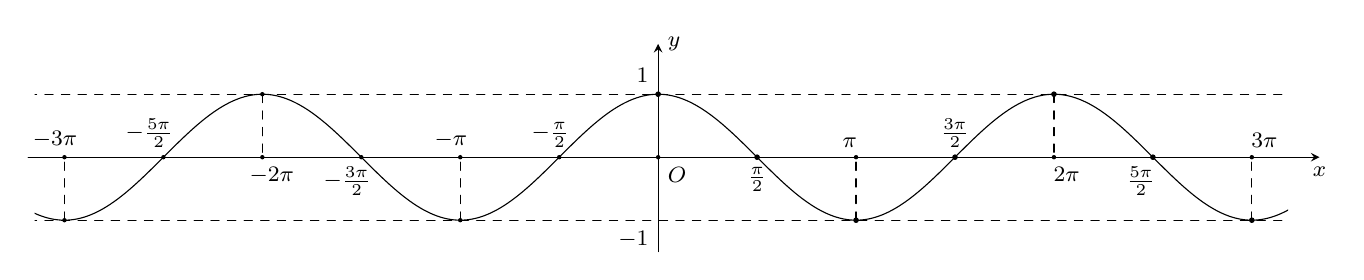
\begin{tikzpicture}[scale=0.8,>=stealth,font=\footnotesize,line join=round,line cap=round]
				\def\xmin{-10} \def\xmax{10.5} \def\ymin{-1.5} \def\ymax{1.8} 
				\draw[->] (\xmin,0)--(\xmax,0) node  [below]{$x$};
				 \draw[->] (0,\ymin)--(0,\ymax) node [right]{$y$};
				\fill (0,0) circle (1pt) node  [below right]{$O$};
				 \clip (\xmin+0.1,\ymin) rectangle (\xmax-0.5,\ymax-0.15);
				\draw[smooth,samples=400,domain=\xmin:\xmax] plot (\x,{cos  (\x r)});
				 \draw[dashed] (\xmin,1)--(\xmax,1)
					 (\xmin,-1)--(\xmax,-1);
				\foreach  \x in {-3*pi,-2.5*pi,-2*pi,-1.5*pi,-pi,-0.5*pi,0}
					{\fill (\x,cos \x*180/pi) circle (1pt); 
				\draw[dashed]  (\x,cos \x*180/pi)--(\x,0);
				\draw[fill]  (-\x,cos -\x*180/pi) circle (1pt);
				\draw[dashed] (-\x,cos \x*180/pi)--(-\x,0);} 
				\foreach \x  in {-3*pi,-2*pi,-pi,pi,2*pi,3*pi}
				\fill (\x,0) circle (1pt); 
				\node at (0,1.3)  [left]{$1$};
				\node at (0,-1.3)  [left]{$-1$};
				\node at  (-2*pi+0.15,0) [below]{$-2\pi$};
				 \node at (-3*pi-0.15,0) [above]{$-3\pi$};
				 \node at (-2.4*pi,0) [above left]{$-\frac{5\pi}{2}$};
				\node  at (-1.4*pi,0) [below left]{$-\frac{3\pi}{2}$};
				 \node at (-pi-0.15,0) [above]{$-\pi$};
				\node at (-0.4*pi,0)  [above left]{$-\frac{\pi}{2}$};
				\node at (0.5*pi,0)  [below]{$\frac{\pi}{2}$};
				\node at (pi-0.1,0) [above]{$\pi$}; 
				\node  at (1.5*pi,0) [above]{$\frac{3\pi}{2}$};
				\node at (2*pi+0.2,0) [below]{$2\pi$}; 
				 \node at (2.5*pi+0.2,0) [below left]{$\frac{5\pi}{2}$};
				\node  at (3*pi+0.2,0) [above]{$3\pi$};
			\end{tikzpicture}
	\end{center}
	Khẳng định nào sau đây  đúng về hàm số $y=f(x)$?
	\choice 
		{Đồ thị trên là đồ thị của hàm  số $y=\sin x$}
		{\True Hàm  số $y=f(x)$ nghịch biến trên khoảng $\left(\dfrac{\pi}{2};\pi\right)$}
		{Đồ thị trên là đồ  thị của hàm số $y=\tan x$}
		{Hàm  số $y=f(x)$ đồng biến trên khoảng $\left(0;\dfrac{\pi}{2}\right)$}
	\loigiai{ Dựa vào đồ thị  ta thấy hàm số $y=f(x)$ nghịch biến trên khoảng $\left(\dfrac{\pi}{2};\pi\right)$.
	 }
\end{ex}

% từ: cau-hoi/lop11/1D1_Ham_so_luong_giac_va_phuong_trinh_luong/1D1-4-7_Bang_bien_thien_va_do_thi.tex
\begin{ex}%[1D1H4-7]%[ma:24eddb5f]
	Hình vẽ bên  dưới là đồ thị của hàm số nào?
	\begin{center}
		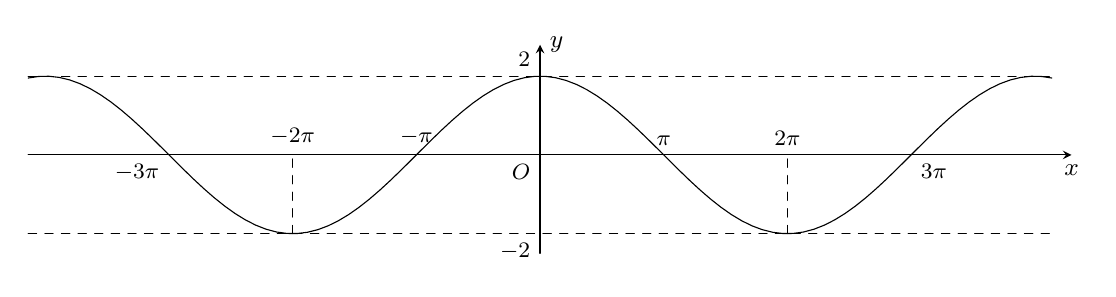
\begin{tikzpicture}[>=stealth,line join=round,line cap=round,font=\footnotesize,scale=0.5]
				\draw[->] (-13,0) --  (13.5,0) node[below] {\small $x$};
				\draw[->]  (0,-2.5) -- (0,2.8) node[right] {\small $y$};
				\draw[samples=100,domain=-13:13]  plot (\x,{2*cos ((\x)*90/pi)});
				\draw  (0,0) node [below left] {$O$};
				\draw  (0,2) node [above left] {$2$};
				\draw (0,-2) node [below left] {$-2$}; 
				 \draw (-pi,0) node[above] {$-\pi$};
				\draw (pi,0)  node[above] {$\pi$};
				\draw[dashed] (-2*pi,-2)--(-2*pi,0) node[above] {$-2\pi$}; 
				\draw[dashed]  (2*pi,-2)--(2*pi,0) node[above] {$2\pi$};
				\draw (-3*pi,0) node[below  left] {$-3\pi$};
				\draw (3*pi,0) node[below right] {$3\pi$}; 
				\draw[dashed] (-13,2)--(13,2); 
				 \draw[dashed] (-13,-2)--(13,-2);
			\end{tikzpicture}
	\end{center}
	\choice 
		{\True $y=2\cos  \dfrac{x}{2}$}
		{$y=\sin  x+2$}
		 {$y=2\sin \dfrac{x}{2}$}
		{$y=1+2\cos x$} 
	\loigiai{ 
		Thử điểm $\left( 0\,;\,1 \right)$ lần lượt vào các hàm số $y=2\cos \dfrac{x}{2}$, $y=\sin x+2$, $y=2\sin \dfrac{x}{2}$, $y=1+2\cos x$ thấy rằng điểm  $\left( 0\,;\,1 \right)$ không thuộc vào đồ thị hai hàm số $y=2\sin \dfrac{x}{2}$ và $y=1+2\cos x$.\\
		Thử điểm $\left( \pi \,;\,0 \right)$ vào hai hàm số $y=2\cos \dfrac{x}{2}$, $y=\sin x+2$ thấy rằng điểm $\left( \pi \,;\,0 \right)$ hông thuộc vào  đồ thị hàm số $y=1+2\cos x$.\\
	Vậy hình vẽ chỉ  có thể là đồ thị hàm số $y=2\cos \dfrac{x}{2}$.}
\end{ex}

% từ: cau-hoi/lop11/1D1_Ham_so_luong_giac_va_phuong_trinh_luong/1D1-4-8_Toan_thuc_te_ap_dung_ham_so_luong_giac.tex
\begin{ex}%[1D1H4-8]%[ma:a78b090c]
	\immini{ 
	Khi đu quay hoạt động, vận tốc theo phương ngang của một  cabin $M$ phụ thuộc vào góc lượng giác $\alpha=(Ox, OM)$ theo hàm số $v_x=0{,}3\sin\alpha$ (m/s).
	\begin{enumerate}
		 \item Tìm giá trị lớn nhất và giá trị nhỏ nhất của $v_x$.
		\item Dựa vào đồ thị của  hàm số sin, hãy cho biết trong vòng quay đầu tiên ($0\leq\alpha\leq 2\pi$), góc $\alpha$ ở trong các khoảng nào thì $v_x$ tăng.
	\end{enumerate}
	} 
	{ 
	\begin{tikzpicture}[scale=0.5,font=\small,line join=round,line cap=round,>=stealth]
			 \tikzset{declare function={g=0;}}
			\coordinate (O) at  (0,0);
			\coordinate[label=above  right:$A$] (A) at (0:4.4);
			 \coordinate[label=above right:$M$] (M) at (30+g:4.4);
			 \pgfmathsetmacro{\gx}{60-g};
			\coordinate (v)  at ($(M)+(120+g:3.3)$);
			\coordinate  (vx) at ($(M)+(180:3.3*cos \gx)$);
			\draw(O)  circle (4.4)
				(O)  circle (3.53);
			\foreach \t in  {0,1,...,11}{
				\draw[very  thick,fill] (O)--(g+30*\t:4.4) circle (0.06);
				\begin{scope}[shift={(g+30*\t:4.4)}]
				\draw[fill=teal]  (-0.27,0)--(0.27,0)--(0.36,-0.18)--(-0.36,-0.18)--cycle
				 (0.32,-0.18)--(0.32,-0.54)
				 (-0.32,-0.18)--(-0.32,-0.54)
				(-0.4,-0.54)--(0.4,-0.54)--(0.27,-1)--(-0.27,-1)--cycle; 
				\end{scope}}
			 \draw[fill=gray!70!yellow] (0.2,0)--(2.35,-5.53)--(3.65,-5.53)--(3.65,-6.02)--(1.95,-6.02)--(0,-0.85)--(-1.95,-6.02)--(-3.65,-6.02)--(-3.65,-5.53)--(-2.35,-5.53)--(-0.2,0)--cycle;
			 \draw[fill=gray!10!yellow] (O) circle (0.34);
			\draw[fill]  (-5,-5.85)--(0,-5.85) circle (0.08)--(6.4,-5.85);
			\draw[->,red] (-5,0)--(6.7,0)  node [below]{\color{black}$x$};
			\draw[->,red] (M)--(v)  node [left=-2pt]{\color{black}$\overrightarrow{v}$};
			\draw[->,red] (M)--(vx)  node [below left=-5pt]{\color{black}$\overrightarrow{v}_{\!\!x}$};
			 \draw (O)--(M);
			\draw[dashed,red]  (0,0)--(0,-5.85)
				(v)--(vx); 
			\fill (0,0) circle (0.1); 
			\path pic[draw=red,angle  radius=5]{right angle=v--M--O}
				(O) pic[draw,->,angle radius=16]{angle=A--O--M}  node[shift={(14:23pt)}]{$\alpha$};
			\node  at (O)[below]{$O$};
		\end{tikzpicture}
	 }
	 \loigiai{
		\begin{enumerate}
			\item Do  $-1\leq\sin\alpha\leq 1$ nên $-0{,}3\leq 0{,}3\sin\alpha\leq 0{,}3$.\\
			Vậy giá trị lớn nhất của $v_x$ là $0{,}3$ (m/s) và giá trị nhỏ nhất của $v_x$  là $-0{,}3$ (m/s).
			\item Ta thấy vòng quay  đầu tiên ($0\le\alpha\leq 2\pi$) thì $v_x$ tăng khi $0\le\alpha\leq \dfrac{\pi}{2}$ và $\dfrac{3\pi}{2}\le\alpha\leq 2\pi$.
		\end{enumerate}
	 }
\end{ex}

% từ: cau-hoi/lop11/1D1_Ham_so_luong_giac_va_phuong_trinh_luong/1D1-4-8_Toan_thuc_te_ap_dung_ham_so_luong_giac.tex
\begin{ex}%[1D1V4-8]%[ma:94898a8c]
	Một cái guồng nước có vành kim loại ngoài cùng là một đường tròn tâm $O$, bán kính là $4$ m. Xét chất điểm $M$ thuộc đường tròn đó và góc $\alpha = (OA, OM)$. Giả sử mực nước lúc đang xét là tiếp xúc với đường tròn $(O;4)$ và guồng nước quay theo chiều dương  (ngược chiều kim đồng hồ). Biết rằng guồng nước quay hết một vòng sau $40$ giây ($t=0$ giây khi điểm $M$ trùng $A$). Hỏi thời điểm nào (trong $1$ vòng quay đầu tiên) thì điểm $M$ ở vị trí cao nhất so với mặt nước?
	\begin{center}
		\begin{tikzpicture}[scale=0.7,font=\small,line join=round,line cap=round,>=stealth]
				\draw[fill=gray!70!yellow] (0.2,0)--(2.35,-5.53)--(3.65,-5.53)--(3.65,-6.02)--(1.95,-6.02)--(0,-0.85)--(-1.95,-6.02)--(-3.65,-6.02)--(-3.65,-5.53)--(-2.35,-5.53)--(-0.2,0)--cycle; 
				\draw[->] (-5,0)--(6.5,0) node  [below]{$x$};
				\draw[->] (0,-5)--(0,6.5)  node [right]{$y$};
				 \tikzset{declare function={g=0;}}
				\coordinate (O) at  (0,0);
				 \coordinate[label=above right:$A$] (A) at (0:4.4);
				\coordinate[label=above right:$M$] (M) at (30+g:4.4); 
				 \pgfmathsetmacro{\gx}{60-g};
				\coordinate (v)  at ($(M)+(120+g:3.3)$);
				 \coordinate (vx) at ($(M)+(180:3.3*cos \gx)$);
				\draw[thick] 
					 (O) circle (4.4)
					(O) circle (3.7) 
					(O) circle (3.1) 
					(O)  circle (2.5);
				\foreach  \t in {0,1,...,11}{
					\draw[very thick,fill] (O)--(g+30*\t:4.4) circle  (0.06);}
				 \draw[fill=gray!10!yellow] (O) circle (0.34);
				 \fill (O) circle (1pt) node[shift={(-15:7mm)}]{$O$};
				 \draw[dashed] (-5,-4.4)--(6.5,-4.4) node[pos=0.85,above]{mặt nước};
				\draw[dashed]  (M)--($(O)!(M)!(0,4.4)$) node[left]{$H$};
				 \draw[dashed] (M)--($(O)!(M)!(A)$) coordinate (K) node[below]{$K$};
				\path[fill=gray,opacity=0.5]  (-5,-4.4) rectangle (6.5,-6.4);
				 \draw[<->] (O)--(-4.4,0) node[sloped,below,pos=0.45]{$4$ m};
				\begin{scope}
					 \clip (K) -- (O) -- (M);
					\draw  (O) circle (1.1cm);
					\draw ($(O)+(0.35,-0.15)$) node[above right]{$\alpha$}; 
				\end{scope}
			\end{tikzpicture}
	\end{center}
	 \loigiai{
		 Gắn guồng nước vào hệ trục tọa độ $Oxy$ như hình vẽ trên.\\
		Khi guồng nước quay theo chiều dương thì điểm $M$ cũng di  động trên đường tròn $(O;4)$ theo chiều dương sao cho $(OA, OM)=\alpha$.\\
		Khi đó $M(x;y)$, với $x=4\cos \alpha$,  $y=4\sin \alpha$.\\
		Điểm $M$ cách mặt nước một khoảng là $h$, với $h=4+y= 4 +  4\sin\alpha$ (m).\\
		Khi $M$ ở vị trí cao nhất so với mặt nước tức là  $h = 8$ thì $\sin\alpha = 1 \Leftrightarrow \alpha = \dfrac{\pi}{2}$ (vì chỉ xét $1$ vòng quay đầu tiên).\\ Thời gian thực hiện của guồng nước là $t = \dfrac{\dfrac{\pi}{2} \cdot 40}{2\pi} = 10$ (giây).
	 }
\end{ex}

% từ: cau-hoi/lop11/1D1_Ham_so_luong_giac_va_phuong_trinh_luong/1D1-5-3_Phuong_trinh_co_ban_dung_Radian.tex
\begin{bt}%[1D1H5-3]%[ma:9ae17101]
% nguon: Archive/2024/TOAN_11_XE/TOAN_11_XE/data4/11C1/KNTT-1.4.tex #1077
%[Tex hóa SGK 11, KNTT]
	Giải các phương trình sau
	\begin{multicols}{2}
		\begin{enumerate}
			\item $\cos x=-\dfrac{\sqrt{3}}{2}$.
			\item  $\cos x=0{,}1$.
		\end{enumerate}
	\end{multicols}	
	\loigiai{
		\begin{enumerate}
			\item $\cos x=-\dfrac{\sqrt{3}}{2} \Leftrightarrow \cos x=\cos \dfrac{5 \pi}{6} \Leftrightarrow x=\pm \dfrac{5 \pi}{6}+k 2 \pi, k \in \mathbb{Z}$.
			\item  Gọi $\alpha \in[0 ; \pi]$ là góc thoả mãn $\cos \alpha=0{,}1$. Khi đó, $$\cos x=0{,}1 \Leftrightarrow \cos x=\cos \alpha \Leftrightarrow x=\pm \alpha+k 2 \pi, k \in \mathbb{Z}.$$
		\end{enumerate}
	}
\end{bt}

% từ: cau-hoi/lop11/1D1_Ham_so_luong_giac_va_phuong_trinh_luong/1D1-5-6_Toan_thuc_te_ap_dung_phuong_trinh_luong_giac.tex
\begin{ex}%[1D1V5-6]%[1D1C5-6]%[ma:b2c2eccf]
	Một vệ tinh bay quanh Trái Đất theo một quỹ đạo hình Elip (như hình vẽ): 
	\begin{center}
		\begin{tikzpicture}[scale=0.2,>=stealth,line join=round,line cap=round,font=\footnotesize,transform shape]
				 \definecolor{customblue}{RGB}{2,47,150}
				 \definecolor{customgreen}{RGB}{46,120,23}
				\path (0,0) coordinate (ea); 
				\fill [ball color=customblue] (ea)  circle (7.57);
				\fill [customgreen] (ea)++(-7.57,0).. controls +(.24,-.32) and +(-.61,-.21).. ++(.8,-1.2) 
					..  controls +(.42,.08) and +(-.24,-.05).. ++(1.3,-1)
					..  controls +(.58,-.32).. ++(1,-.58)
					..  controls +(-.16,-.32) and +(-.74,.56).. ++(1,-1.3)
					.. controls +(.05,-.4) and  +(-.08,.53).. ++(1.1,-.69)
					.. controls +(-.34,-.08) and +(-.08,.56)..  +(.88,-1.3)
					.. controls  +(.13,-.56) and +(-.66,.69).. ++(1.67,-2.01)
					.. controls +(.42,-.05)..  ++(.88,-.21)
					.. controls +(.21,0) and +(.4,-.21)..  ++(-.19,.4)
					 .. controls +(-.19,.9).. ++(-.45,1.08)
					.. controls +(-.19,.16) and  +(-.32,0).. ++(.36,.4)
					.. controls +(.11,.03).. ++(0,.24) 
					.. controls +(.26,.32)..  ++(.34,.74)
					.. controls +(-.45,.66).. ++(.5,.79) 
					.. controls +(-.03,1.53) and +(2.12,-.11).. ++(-1.77,2.04) 
					.. controls +(-.37,.74) and +(.21,-.53)..  ++(-1.27,.66)
					.. controls  +(-.42,.24) and +(.05,.37).. ++(-1.16,-.32)
					.. controls +(-.61,-.13) and  +(.26,-.16).. ++(-.45,.37)
					.. controls +(-.37,.05) and +(.45,.63).. ++(-.71,.11) 
					.. controls +(-.77,0) and  +(-.85,.66).. ++(.63,.77)
					.. controls +(.21,-.32) and +(.34,-.32)..  ++(.08,.24)
					.. controls  +(-.08,.24).. ++(.29,.48)
					.. controls +(.03,.95)..  ++(1.06,1.19)
					..  controls +(.26,.03) and +(.29,0).. ++(-.05,.26)
					.. controls +(.21,.29)  and +(-.08,.29).. ++(.29,0)
					.. controls +(.21,.16)  and +(.34,-.13).. ++(.19,.5)
					.. controls +(.11,.34) and  +(.03,-.32).. ++(-.29,.48)
					..  controls +(.05,.24) and +(.05,.24).. ++(-.26,0)
					.. controls +(-.29,-.13) and  +(.21,.42).. ++(-.61,.03)
					.. controls +(-.24,-.16)  and +(.32,.21).. ++(-.29,-.63)
					.. controls +(.16,-.37)  and +(.4,-.45).. ++(-.74,.08)
					..  controls +(.26,.45) and +(-.21,-.48).. ++(1.19,1.48)
					.. controls +(.45,-.29) and +(-.08,.26).. ++(.05,-.5) 
					.. controls +(.34,.03) and +(-.03,-.5)..  ++(.74,.29)
					.. controls +(.29,.19) and  +(.69,-.11).. ++(-.32,.48)
					.. controls  +(-.26,.26) and +(-.61,-.48).. ++(.58,1.06)
					.. controls  +(.4,.08) and +(-.74,-.56).. ++(.24,-.24)
					..  controls +(.74,.19) and +(-1.32,-2.43).. ++(1.19,-.4)
					.. controls +(.71,.19).. ++(1.22,1.08) 
					.. controls +(-.13,.11)..  ++(.24,.29)
					.. controls +(.03,.24)..++(.34,.58) 
					 .. controls +(-.21,.16).. ++(-.37,-.13)
					..  controls +(-.4,.11) and +(1.22,.77).. ++(-2.12,-.79)
					.. controls +(-.56,.24) and +(.45,.24)..  ++(-1.69,.77)
					.. controls +(-.79,-.58) and +(.45,-.03).. ++(-.74,-1.11) 
					.. controls +(-.05,.24) and  +(-.08,.5).. ++(-.32,.42)
					.. controls +(-.03,-.16) and +(.19,-.27).. ($(ea)+(127:7.57)$) arc (127:180:7.57) 
					(ea)++(7.5,.99).. controls +(-.46,.68) and +(.37,-.5)..  ++(-1.39,.55)
					..  controls +(-.32,.56) and +(-.53,.48).. ++(-.05,-.29)
					.. controls +(.63,-.03) and  +(1.71,1.01).. ++(-.42,-1.08)
					.. controls +(-.82,1.75) and +(-1.64,2.06)..  ++(-.19,-.11)
					.. controls +(.85,.16) and +(1.32,1.03).. ++(-.29,-1.24) 
					.. controls  +(-.26,-.5) and +(1.06,.5).. ++(-.63,-1.72)
					..  controls +(.13,-.79) and +(1.24,.13).. ++(-1.64,-1.88)
					..  controls +(.19,.53).. ++(-.4,1.8)
					..  controls +(.19,.53) and +(-.16,-.77).. ++(-.26,1.4)
					.. controls +(-.5,.63)  and +(.85,-.95).. ++(-.34,2.12)
					.. controls  +(.34,.71) and +(1.03,-.03).. ++(-.93,.71)
					..  controls +(-2.06,-.32) and +(.79,-.29).. ++(-1.88,.61)
					.. controls +(-.37,.24) and +(.29,-.42).. ++(0,1.01) 
					.. controls +(1.01,1.51)  and +(-1.83,.03).. ++(2.83,1.48)
					.. controls +(.13,-.42) and  +(-.77,-.42).. ++(1.11,-.37)
					.. controls +(.21,-.34)  and +(-.34,-.16).. ++(1.06,-.24)
					 .. controls +(.42,.42) and +(.4,.21).. ++(-.21,.37)
					 .. controls +(-.29,-.08) and +(-.08,-.26).. ++(-.45,.4)
					.. controls +(-.21,.32) and +(.05,-.61)..  ++(-.45,.08)
					.. controls +(-.98,1.08) and +(-.48,.21)..  ++(-.32,.08)
					.. controls +(.19,-.16) and +(.29,.13)..  ++(-.4,-.4)--++(-.09,.13)
					 .. controls +(.26,.16) and +(.16,-.08).. ++(-.21,.69)
					..  controls +(-.19,-.08) and +(.32,.26).. ++(-.63,-.19)
					.. controls +(-.29,-.11) and +(1.14,-.37)..  ++(-1.35,-.32)
					.. controls +(.11,.53) and +(-.34,.11).. ++(.61,.56) 
					.. controls +(-.03,.13)  and +(.32,-.24).. ++(.03,.4)
					.. controls +(.66,.13).. ++(.74,.45) 
					.. controls +(.4,.05).. ++(.4,.45) 
					.. controls +(.24,-.29) and +(-.11,-.69)..  ++(.98,.03)
					.. controls +(.56,.24)  and +(-.34,-.45).. ($(ea)+(69:7.57)$) arc (69:8:7.57)
					 (ea)++(5.37,-2.67)
					.. controls +(-.26,-1.08) and +(-.37,-1.14)..  ++(.4,-.29)
					.. controls +(.32,.69) and +(.45,.63).. ++(-.4,.29) 
					(ea)++(1.6,6.9).. controls  +(.98,.21) and +(.13,.19).. ++(.69,-.26)
					.. controls  +(-.66,.03) and +(-.32,-.37).. ++(-.69,.26);
				\path 
					 (ea)++(0:2) coordinate (O)
					($({11*cos  (65)},{8.5*sin (65)})+(O)$) coordinate (V)
					 (ea)++(50:7.57) coordinate (V1)
					($({11*cos (-80)},{8.5*sin (-80)})+(O)$)  coordinate (V2)
					(ea)++(-65:7.57) coordinate (V3); 
				\draw (O) ellipse (11  and 8.5);
				\draw  [<->] (7.57,0)--(13,0) node [below,midway] {\scalebox{4}{1\,000}};
				\draw [<-] (-9,0)--++(180:2) node [pos=1,left]  {\scalebox{4}{$h=100$}};
				\draw  [<-] (-7.57,0)--++(0:2);
				\draw [<->] (V)--(V1) node [midway,below right] {\scalebox{4}{$h$}}; 
				\draw [<->] (V2)--(V3) node [midway,above=25pt,sloped] {\scalebox{4}{$250$}}; 
				\draw [fill=white] (V) circle (4pt) node [above right]  {\scalebox{4}{Vệ tinh}};
			\end{tikzpicture}
	\end{center}
	Độ cao $h$ (tính bằng kilômet) của vệ tinh so với bề  mặt Trái Đất được xác định bởi công thức $h=550+450\cdot\cos\dfrac{\pi}{50}t$. Trong đó $t$ là thời gian tính bằng phút kể từ lúc vệ tinh bay vào quỹ đạo. Người ta cần thực hiện một thí nghiệm khoa học khi vệ tinh cách mặt đất $250$ km. Trong khoảng $60$ phút đầu tiên kể từ lúc vệ tinh bay vào quỹ đạo, hãy tìm thời điểm để có thể thực hiện thí nghiệm đó?
	\loigiai{ 
		Ta có 
		\begin{align*}
			550+450\cdot\cos\dfrac{\pi}{50}t=250 &\Leftrightarrow \cos\dfrac{\pi}{50}t=-\dfrac{2}{3}.\\ 
			\text{(bấm máy) }\hoac{&\dfrac{\pi}{50}t\approx 2{,}3+k2\pi\\&\dfrac{\pi}{50}t\approx -2{,}3+k2\pi} 
			&\Leftrightarrow 
			\hoac{&t\approx  36{,}61+k100\\&t\approx -36{,}61+k100},k\in \mathbb{Z}.
		\end{align*}
		Vậy trong khoảng $60$ phút  đầu tiên kể từ lúc vệ tinh bay vào quỹ đạo, tại thời điểm $t\approx 36{,}61$ (phút) thì ta có thể thực hiện thí nghiệm đó.
	} 
\end{ex}

% từ: cau-hoi/lop11/1D1_Ham_so_luong_giac_va_phuong_trinh_luong/1D1-5-6_Toan_thuc_te_ap_dung_phuong_trinh_luong_giac.tex
\begin{ex}%[1D1V5-6]%[1D1C5-6]%[ma:780040d4]
	Một chất điểm chuyển động đều theo chiều ngược chiều kim đồng hồ trên đường tròn bán kính $5$ cm. Khoảng cách $h$ cm từ chất điểm đến trục hoành được tính theo  công thức $h=\big|y\big|$, trong đó $y=a\sin\left( \dfrac{\pi}{5}t \right)$ với $t$ là thời gian chuyển động của chất điểm tính bằng giây $( t\ge 0)$ và chất điểm bắt đầu chuyển động từ vị trí $A$.
	\begin{enumerate}
		\item Chất điểm chuyển động một vòng hết bao nhiêu  giây?
		\item Tìm giá trị của  $a$.
		\item Tìm thời điểm sao cho chất điểm ở vị trí có $h=2{,}5$ cm và nằm  phía dưới trục hoành trong một vòng quay đầu tiên.
		\begin{center}
			\begin{tikzpicture}[scale=1,>=stealth,font=\footnotesize,line join=round,line cap=round,x=3mm,y=3mm]
					\def\xmin{-7} \def\xmax{7} 
					\def\ymin{-7} \def\ymax{7} 
					\draw[->] (\xmin,0)--(\xmax,0) node [below]{$x$}; 
					\draw[->] (0,\ymin)--(0,\ymax) node  [left]{$y$};
					\node at  (0,0) [below left]{$O$};
					\path (0,0)  coordinate (O)
						 (0:5) coordinate (A)
						 (45:5) coordinate (B)
						 ($(O)!(B)!(A)$) coordinate (H);
					\draw[cyan] (0,0)  circle (5);
					\draw[dashed]  (O)--(B) node[midway,above]{$5$}--(H) node[midway,left]{$h$};
					\draw[black,fill] (O) circle  (1.25pt)
						 (A) circle (1.25pt)
						(B)  circle (1.25pt)
						(H) circle (1.25pt); 
					\path  (B) node[above right]{$A$};
				\end{tikzpicture}
		\end{center}
	\end{enumerate}
	\loigiai{ 
		\begin{enumerate}
			\item Xét $h=0$ hay  $a\sin\left( \dfrac{\pi}{5}t \right)=0 \Leftrightarrow t=5k$ với $k\in \mathbb{Z}$ và $k\ge 0$.\\
			Ta nhận thấy, từ thời điểm ban đầu, cứ sau $5$ giây, khoảng cách từ chất điểm đến trục  hoành lại bằng $0$.\\
			Suy ra sau mỗi $5$ giây, chất điểm chuyển động được nửa vòng.\\ 
			Vậy chất điểm chuyển động một vòng hết 10 giây. 
			\item Do chất điểm chuyển động một vòng hết $10$ giây nên khi $t=2{,}5$ giây thì chất điểm chuyển động được  một phần tư vòng theo chiều dương, suy ra tại $t=2{,}5$ ta có \\
			\centerline{$y=\big|y\big|=h=5 \Leftrightarrow a\sin\left(\dfrac{\pi}{5}\cdot\dfrac{5}{2}\right) =5  \Leftrightarrow a=5$.
			} 
			\item Khi chất điểm nằm phía dưới trục hoành và có vị trí $h=2{,}5$ cm  ta có
			\begin{eqnarray*}
				&&y=-2{,5} \\ 
				&\Leftrightarrow& 5\sin\left(\dfrac{\pi}{5}t\right)=2{,5}  \\
				&\Leftrightarrow&  \sin\left(\dfrac{\pi}{5}t\right)=\dfrac{1}{2} \\
				&\Leftrightarrow&  \sin\left(\dfrac{\pi}{5}t\right)=\sin\dfrac{\pi}{6} \\
				&\Leftrightarrow& \hoac{&\dfrac{\pi}{5}t=\dfrac{\pi}{6}+k2\pi \\ &\dfrac{\pi}{5}t=\dfrac{5\pi}{6}+k2\pi}, \quad k\in  \mathbb{Z} \\
				 &\Leftrightarrow& \hoac{&t=\dfrac{5}{6}+10k \\ &t=\dfrac{25}{6}+10k.}
			\end{eqnarray*}
			Vì là thời điểm đầu tiên nên $t$ nhận giá trị không âm và  nhỏ nhất. \\
			Do đó $t=\dfrac{5}{6}$.  \\
			Vậy thời điểm  đầu tiên chất điểm ở vị trí $h=2{,}5$ và phía dưới trục hoành là $\dfrac{5}{6}$ (giây).
		\end{enumerate}
	} 
\end{ex}

% từ: cau-hoi/lop11/1D1_Ham_so_luong_giac_va_phuong_trinh_luong/1D1-5-6_Toan_thuc_te_ap_dung_phuong_trinh_luong_giac.tex
\begin{ex}%[1D1V5-6]%[ma:ee15a5d2]
	Trong hình minh hoạ dưới đây, cây xanh $AB$ nằm trên đường xích đạo được trồng vuông góc với mặt đất và có chiều cao $5$ m. Bóng của cây là $BE$. Vào ngày xuân phân và hạ phân, điểm $E$ di chuyển trên đường thẳng $Bx$. Góc thiên đỉnh $\theta_x=(AB,AE)$ phụ thuộc vào vị trí của Mặt Trời và thay đổi theo thời gian trong ngày theo công thức: $\theta_s=\dfrac{\pi}{12}(t-12)$, với $t$ là thời gian trong ngày (theo đơn vị giờ, $6<t<18)$. 
	\begin{center}
	 \usetikzlibrary{decorations.pathmorphing,shapes}
		\tikzset{ 
		treetop/.style = { 
		 decoration={random steps, segment length=0.4mm},
		decorate 
		}, 
		 trunk/.style = {
		decoration={random steps, segment length=2mm, amplitude=0.2mm}, 
		 decorate
		 }
		 }
		\begin{tikzpicture}[scale=.6]
				\path 
					(0,-3) coordinate (B) 
					(0,1.45) coordinate (A) 
					 (-3.6,-3) coordinate (N)
					 (3.2,-3) coordinate (E);
				\foreach \w/\f  in {0.3/30,0.2/50,0.1/70}{
					\fill [brown!\f!black,trunk]  (0,0) ++(-\w/2,0) rectangle +(\w,-3);
				 }
				\foreach  \n/\f in {1.4/40,1.2/50,1/60,0.8/70,0.6/80,0.4/90}{
					 \fill [green!\f!black,treetop] ellipse (\n/1.5 and \n);
				} 
				\draw[dashed] (A)--(B) node[left=0.5cm,midway]{$5$ m}; 
				\path ($(N)!.5!(B)$)  node[below]{$4$ m};
				 \draw[] (A)--(E);
				\draw[pattern=north east  lines,pattern color=red] (N) rectangle ($(N)+(-.7,2.5)$);
				\path pic[draw,angle radius=20pt]{angle=  B--A--E};
				 \foreach \t/\g in {A/90,B/-90,N/-90,E/-90}{
					 \draw[fill=red,draw=black] (\t) circle (1pt) node[shift={(\g:7pt)}]{$\t$};
				 }
				\path (A)+(-70:15pt)  node[sloped]{$\theta_s$};
				\draw[-stealth,ultra thick]  (-5,-3)--(4.5,-3) node[above]{$x$(m)};
			\end{tikzpicture}
	\end{center}
	\begin{enumerate}
		\item Viết hàm  số biểu diễn toạ độ của điểm $E$ trên trục $Bx$ theo $t$.
		\item Dựa vào đồ thị hàm số tang, hãy xác định các thời điểm mà tại đó bóng cây phủ qua vị trí tường rào $N$ biết  $N$ nằm trên trục $Bx$ với toạ độ là $x_N=-4$ (m). (Làm tròn kết quả đến hàng phần mười).
	\end{enumerate}
	 \loigiai{
		\begin{enumerate}
			\item Xét tam giác $ABE$ vuông  tại $B$ ta có $\tan\theta_s=\dfrac{BE}{AB}\Leftrightarrow BE=5\tan\left(\dfrac{\pi}{12}(t-12)\right)$.
			\item  Đồ thị của hàm số $\theta_s=5\tan\left(\dfrac{\pi}{12}(t-12)\right)$.\\
			Dựa vào đồ  thị hàm số để $\theta_s=5\tan\left(\dfrac{\pi}{12}(t-12)\right) <-4$ và $6<t<18$ suy ra các thời điểm để bóng cây phủ qua hàng rào $N$ là $6<t<9{,}4$.
	\end{enumerate}}
\end{ex}

% từ: cau-hoi/lop11/1D1_Ham_so_luong_giac_va_phuong_trinh_luong/1D1-5-6_Toan_thuc_te_ap_dung_phuong_trinh_luong_giac.tex
\begin{ex}%[1D1C5-6]%[ma:27b0bf56]
	Một chiếc guồng nước có dạng hình tròn bán kính $2{,}5$ m; trục của nó đặt cách mặt nước $2$ m (hình bên). Khi guồng quay đều, khoảng cách $h$ (mét) tính từ một chiếc gầu gắn tại điểm $A$ trên guồng đến mặt nước là $h=\big|y\big|$ trong đó $y=2+2,5\sin 2\pi \left( x-\dfrac{1}{4} \right)$ với $x$ là thời gian  quay của guồng $(x\ge 0)$, tính bằng phút; ta quy ước rằng $y>0$ khi gầu ở trên mặt nước và $y<0$ khi gầu ở dưới mặt nước.
	\begin{enumerate}
		\item Khi  nào chiếc gầu ở vị trí cao nhất? Thấp nhất?
		\item Chiếc gầu cách mặt nước 2 mét lần đầu tiên khi  nào? \\
		 \centerline{
		\begin{tikzpicture}[>=stealth,line cap=round,line join=round,font=\footnotesize,x=8mm,y=8mm]
				\path  (0:0) coordinate (O)
					(30:2.5) coordinate (A) 
					(-4,-2) coordinate (x') 
					(4,-2) coordinate  (x)
					 ($(x')!(A)!(x)$) coordinate (H)
					($(x')!(O)!(x)$) coordinate  (I);
				\draw[dashed] (x')--(x) 
					 (A)--(H);
				\draw[]  (O) circle (2.5);
				\draw[->,cyan] (45:2.85)  arc (45:75:2.85);
				\draw[<->] (O)--(A) node[above,midway,sloped]  {$2{,}5$m};
				\draw[<->] (O)--(I) node[left,midway]  {$2$m};
				\foreach \x/\y  in {A/45}
				\fill  (\x) circle (1pt)
					($(\y:3mm)+(\x)$) node  {$\x$};
				 \foreach \x in {O,H,I}
				\fill (\x) circle  (1pt);
				\path (0,-2.5) node[below]  {Mô phỏng guồng nước};
			\end{tikzpicture}
		\hspace*{1cm} 
		\begin{tikzpicture}[scale=0.7,font=\footnotesize,line join=round,line cap=round,>=stealth]
				\def\r{3} 
				\path 
					 (0,0) coordinate (O)
					(O)++(30:\r) coordinate (M) 
					(O)++(30:\r*1.5)  coordinate (H)
					(O)++(45:\r*4/3)++(90:\r/3) coordinate (O') 
					(O)++(-80:\r/5) coordinate  (T1) arc (-80:-100:\r/5) coordinate (T2)
					(O)++(-90:\r*1.5)  coordinate (H)
					(H)++(180:0.5) coordinate (T3) 
					(H)++(0:0.5) coordinate (T4); 
				\fill  [black!80] (T1)--(T2)--(T3)--(T4);
				 \path [fill=gray!50]
					(O)++(42:\r*2/3) coordinate (G1) 
					(G1)++(12:\r/6) coordinate (G2) 
					(O)++(42:\r) coordinate (G3) 
					(G1) arc (42:60:\r*2/3) coordinate  (G5)++(30:\r/6) coordinate (G4)
					($(G3)!1/2!(G4)$) coordinate  (X)
					(G1) arc (42:60:\r*2/3)--(G4)..  controls ++(10:0.2).. (X).. controls ++(-10:0.2).. (G3)--(G2)--(G1)
					($(G3)!1/6!(G4)$)  coordinate (Ga)
					 ($(G3)!5/6!(G4)$) coordinate (Gb);
				\foreach  \x in {0,20,...,360}{
					\draw (O)++(\x:2/3*\r)--++(\x-30:\r/6)--($(O)+(\x:\r)$); 
					 \draw (O)++(\x+2:2/3*\r)--++(\x-28:\r/6)--($(O)+(\x+2:\r)$)--($(O)+(\x:\r)$);
				 }
				 \def\ga{0}
				\def\gb{150} 
				\def\gc{45} 
				 \fill [gray!50] (O')--++(\ga+150:\r*4/3/8)--++(\ga+45:{\r*4/3/12*sqrt (2)})--++(-45+\ga:{\r*4/3/12*sqrt (2)})--cycle;
				\draw  [fill=gray!90] ($(O')+(\ga+150:\r*4/3/8)$)--++(\ga+45:{\r*4/3/10*sqrt (2)})--++(\ga:9*\r*4/3/10)--++(-90+\ga:{\r*4/3/10})--cycle
					(O')--++(\ga+150:\r*4/3/8); 
				\draw [fill=gray!90] (O')--++(\ga:\r*4/3)--++(90+\ga:\r*4/3/10)--++(-180+\ga:9*\r*4/3/10)--cycle; 
			\fill [gray!50,draw] (O') parabola (Ga).. controls ++(-10:0.2).. (Gb) parabola [bend at end] ($(O')+(\gb:\r*4/3/8)$);
			 \foreach \x in {0,45,...,360}{
				\draw  (O)++(\x-10:\r/5)--($(O)+(\x-2:2/3*\r)$);
				\draw (O)++(\x+10:\r/5)--($(O)+(\x+2:2/3*\r)$); 
			} 
			\draw [gray,line width=2pt] (O) circle  (\r);
			\draw [gray,line width=2pt] (O)  circle (2/3*\r);
			\draw [fill=gray] (O) circle  (\r/5);
			 \fill
				(O)  circle (1pt)
				 (M) circle (1pt)
				 (H) circle (1pt);
		\end{tikzpicture}
		} 
	\end{enumerate}
	\loigiai{ 
		\begin{enumerate}
			\item 
			Ta có $-1\le \sin 2\pi \left( x-\dfrac{1}{4} \right)\le 1 \Rightarrow -2{,}5\le 2{,}5\sin 2\pi \left( x-\dfrac{1}{4} \right)\le  2{,}5$.\\
			Do đó  $-2{,}5+2\le 2+2{,}5\sin 2\pi \left( x-\dfrac{1}{4} \right)\le 2{,}5+2 \Rightarrow 0{,}5\le y \le 4{,}5$, $\forall x\in \mathbb{R}$.\\
			Suy ra, gầu ở vị tri cao nhất  $y=4{,}5$
			\begin{eqnarray*}
				& &\sin 2\pi \left( x-\dfrac{1}{4}  \right) =1\\
				& \Leftrightarrow& 2\pi  \left( x-\dfrac{1}{4} \right) =\dfrac{\pi }{2}+k2\pi\\
				& \Leftrightarrow& x=\dfrac{1}{2}+k\  \left( k\in \mathbb{Z} \right)\\
				& \Rightarrow & x\in \left\{\dfrac{1}{2}, \dfrac{3}{2}, \dfrac{5}{2},  \ldots\right\}.
			\end{eqnarray*}
			Vậy gầu ở vị trí cao nhất tại các thời  điểm $\dfrac{1}{2},\dfrac{3}{2},\dfrac{5}{2},\ldots $ phút.\\
			Tương tự, gầu  ở vị trí thấp $y=0{,}5$
			\begin{eqnarray*}
				& &\sin 2\pi \left( x-\dfrac{1}{4} \right) =-1\\ 
				& \Leftrightarrow& 2\pi  \left( x-\dfrac{1}{4} \right) =-\dfrac{\pi }{2}+k2\pi\\
				& \Leftrightarrow& x=k\ \left(  k\in \mathbb{Z} \right)\\
				& \Rightarrow & x\in \left\{0, 1,  2, 3, \ldots\right\}.
			\end{eqnarray*}
			Vậy gầu ở vị trí thấp nhất tại các thời điểm $0,1,2,3,\ldots  $ phút.
			\item Gầu cách mặt nước $2$ m khi\\ 
			$2+2{,}5\sin 2\pi \left( x-\dfrac{1}{4} \right)=2$ $\Leftrightarrow \sin 2\pi \left( x-\dfrac{1}{4} \right)=0 \Leftrightarrow 2\pi \left( x-\dfrac{1}{4}  \right) =k\pi \Leftrightarrow x=\dfrac{1}{4}+\dfrac{k}{2} \left( k\in \mathbb{Z} \right)$.\\
			Vậy chiếc gầu cách mặt nước $2$ m lần đầu tiên  tại thời điểm $x=\dfrac{1}{4}$ phút $=15$ giây.
		\end{enumerate}
	} 
\end{ex}

% từ: cau-hoi/lop11/1D1_Ham_so_luong_giac_va_phuong_trinh_luong/1D1-5-6_Toan_thuc_te_ap_dung_phuong_trinh_luong_giac.tex
\begin{bt}%[1D1V5-6]%[ma:e530de37]
% nguon: Archive/2024/TOAN_11_XE/TOAN_11_XE/data4/11C1/KNTT-1.OTC.tex #1120
%[Trần Công Duy]
	Trong hình vẽ, cây xanh $AB$ nằm trên đường xích đạo được trồng vuông góc với mặt đất và có chiều cao $5 \mathrm{~m}$. Bóng của cây là $B E$. Vào ngày xuân phân và hạ phân, điểm $E$ di chuyển trên đường thẳng $B x$. Góc thiên đỉnh $\theta_s=(AB, AE)$ phụ thuộc vào vị trí của Mặt Trời và thay đổi theo thời gian trong ngày theo công thức
	$$
	\theta_s(t)=\dfrac{\pi}{12}(t-12)\, \mathrm{rad}
	$$
	với $t$ là thời gian trong ngày (theo đơn vị giờ, $6<t<18)$.\\
	\mbox{}\hfill (Theo \textit{https://www.sciencedirect.com/ topics/engineering/solar-hour-angle})
	\usetikzlibrary{decorations.pathmorphing,shapes}
	\tikzset{
		treetop/.style = {
			decoration={random steps, segment length=0.4mm},
			decorate
		},
		trunk/.style = {
			decoration={random steps, segment length=2mm, amplitude=0.2mm},
			decorate
		}
	}
	\begin{center}
		\begin{tikzpicture}
			\path 
			(0,-3) coordinate (B)
			(0,1.45) coordinate (A)
			(-3.6,-3) coordinate (N)
			(3.2,-3) coordinate (E)
			;
			\foreach \w/\f in {0.3/30,0.2/50,0.1/70} {
				\fill [brown!\f!black, trunk] (0,0) ++(-\w/2,0) rectangle +(\w,-3);
			}
			\foreach \n/\f in {1.4/40,1.2/50,1/60,0.8/70,0.6/80,0.4/90} {
				\fill [green!\f!black, treetop] ellipse (\n/1.5 and \n);
			}
			
			\draw[dashed] (A)--(B) node[left=1cm,midway]{$5$ m};
			\path ($(N)!.5!(B)$)node[below]{$4$ m};
			\draw[] (A)--(E);
			\draw[pattern=north east lines,pattern color=red] (N) rectangle ($(N)+(-.7,1.5)$);
			\path pic[draw,angle radius=20pt]{angle= B--A--E};
			\foreach \t/\g in {A/90, B/-90,N/-90,E/-90}{
				\draw[fill=red,draw=black] (\t) circle (1pt) node[shift={(\g:7pt)}]{$ \t $};
			}
			\path (A)+(-70:15pt)node[sloped]{$\theta_s$};
			\draw[-stealth,ultra thick] (-5,-3)--(4.5,-3)node[below]{$x$ (m)};
		\end{tikzpicture}
	\end{center}
	\begin{listEX}
		\item Viết hàm số biểu diễn toạ độ của điểm $E$ trên trục $Bx$ theo $t$.
		\item Dựa vào đồ thị hàm số tang, hãy xác định các thời điểm mà tại đó bóng cây phủ qua vị trí tường rào $N$ biết $N$ nằm trên trục $B x$ với toạ độ là $x_N=-4$ (m). Làm tròn kết quả đến hàng phần mười.
	\end{listEX}
	\loigiai{
		\begin{listEX}
			\item Hàm số biểu diễn toạ độ của điểm $E$ trên trục $Bx$ theo $t$ là
			\allowdisplaybreaks
			\begin{eqnarray*}
				x_E=\overline{BE}=AB\cdot \tan \theta_s(t)=5\tan\dfrac{\pi}{12}(t-12)\, (m).
			\end{eqnarray*}			
			\item 
			Gọi $t_N$ là thời điểm bóng cây phủ đến vị trí $N$, khi đó $t_N$ là nghiệm của phương trình 
			\allowdisplaybreaks
			\begin{eqnarray*}
				&&5\tan\dfrac{\pi}{12}(t_N-12) = -4 \\
				&\Leftrightarrow& \tan\dfrac{\pi}{12}(t_N-12) =-\dfrac{4}{5}\\
				& \Leftrightarrow& \dfrac{\pi}{12}(t_N-12)\approx -0{,}675+k\pi \\
				&\Leftrightarrow& t_N\approx \dfrac{-0{,}675}{\dfrac{\pi}{12}}+12+12k \approx 9{,}4+12k.
			\end{eqnarray*}	
			Vì $6<t_N<18$ nên $k=0$; Lúc đó $t_N=9{,}4$ (giờ).\\
			Với $6<t<18$ thì $-\dfrac{\pi}{2}<\dfrac{\pi}{12}(t-12)<\dfrac{\pi}{2}$. Suy ra hàm số $x_E$ đồng biến trên $(6;18)$.\\
			Bóng cây phủ qua vị trí tường rào $N$ khi và chỉ khi
			\allowdisplaybreaks
			\begin{eqnarray*}
				x_E\leq x_N \Leftrightarrow t\leq t_N=9{,}4\,\text{(giờ)}.
			\end{eqnarray*}	
			Vậy các thời điểm bóng cây phủ qua vị trí tường rào $N$ là từ hơn $6$ giờ đến $9{,}4$ giờ.
		\end{listEX}
		
	}
\end{bt}

% từ: cau-hoi/lop11/1D1_Ham_so_luong_giac_va_phuong_trinh_luong/1D1-6-1_Phuong_trinh_bac_n_theo_mot_ham_so_luong_giac.tex
\begin{bt}%[1D1H6-1]%[ma:baa4c614]
% nguon: Archive/SP_KhoLatex/ID6_old/1K1-4-7.tex #3455

	Giải các phương trình lượng giác sau:
	\begin{listEX}[2]
		\item $2\cos^2{2x}+5\sin{2x}+1=0$.
		%		 \dapso{$\hoac{&x=\dfrac{-5\pi}{12}+k\pi\\&x=\dfrac{-\pi}{12}+k\pi}(k\in\mathbb{Z})$}
		\item $5\cos{x}-2\sin\dfrac{x}{2}+7=0$.
		%		 \dapso{$x=\pi+4k\pi\,(k\in\mathbb{Z})$}
		\item $\sin^2{x}+\cos{2x}+\cos{x}=2$.
		%		 \dapso{$x=k2\pi\,(k\in\mathbb{Z})$}
		\item $\cos{2x}+\cos^2{x}-\sin{x}+2=0$.
		%		 \dapso{$x=\dfrac{\pi}{2}+k2\pi\,(k\in\mathbb{Z})$}
	\end{listEX}
	\loigiai{
		\begin{listEX}[2]
			\item! Ta có
			$$
			2\cos^2{2x}+5\sin{2x}+1=0 \Leftrightarrow -2\sin^2{2x}+5\sin{2x}+3=0.
			$$
			Đặt $t=\sin{2x}\,(-1\le t\le 1)$. Khi đó, phương trình trở thành:
			$$
			2t^2-5t-3=0 \Leftrightarrow \hoac{&t=3\\&t=\dfrac{-1}{2}.}
			$$
			Vì $-1\le t\le 1$ nên $t=\sin{2x}=\dfrac{-1}{2}\Leftrightarrow \hoac{&x=\dfrac{-5\pi}{12}+k\pi\\&x=\dfrac{-\pi}{12}+k\pi}(k\in\mathbb{Z})$.
			\item! Đặt $y=\dfrac{x}{2}$. Khi đó, phương trình trở thành:
			$$
			5\cos{2y}-2\sin{y}+7=0 \Leftrightarrow -10\sin^2{y}-2\sin{y}+12=0.
			$$
			Đặt $t=\sin{y}\,(-1\le t\le 1)$. Khi đó, phương trình trở thành:
			$$
			10t^2+2t-12=0 \Leftrightarrow \hoac{&t=1\\&t=\dfrac{-6}{5}.}
			$$
			Vì $-1\le t\le 1,y=\dfrac{x}{2}$ nên $t=\sin\dfrac{x}{2}=1\Leftrightarrow x=\pi+4k\pi\,(k\in\mathbb{Z})$.
			\item! Ta có
			\begin{eqnarray*}
				& \sin^2{x}+\cos{2x}+\cos{x}=2 & \Leftrightarrow 1-\cos^2{x}+2\cos^2{x}-1+\cos{x}-2=0\\
				& & \Leftrightarrow \cos^2{x}+\cos{x}-2=0.
			\end{eqnarray*}
			Đặt $t=\cos{x}\,(-1\le t\le 1)$. Khi đó, phương trình trở thành:
			$$
			t^2+t-2=0 \Leftrightarrow \hoac{&t=-2\\&t=1.}
			$$
			Vì $-1\le t\le 1$ nên $t=\cos{x}=1\Leftrightarrow x=k2\pi\,(k\in\mathbb{Z})$.
			\item! Ta có
			\begin{eqnarray*}
				& \cos{2x}+\cos^2{x}-\sin{x}+2=0 & \Leftrightarrow 1-2\sin^2{x}+1-\sin^2{x}-\sin{x}+2=0\\
				& & \Leftrightarrow 3\sin^2{x}+\sin{x}-4=0.
			\end{eqnarray*}
			Đặt $t=\sin{x}\,(-1\le t\le 1)$. Khi đó, phương trình trở thành:
			$$
			3t^2+t-4=0 \Leftrightarrow \hoac{&t=\dfrac{-4}{3}\\&t=1.}
			$$
			Vì $-1\le t\le 1$ nên $t=\sin{x}=1\Leftrightarrow x=\dfrac{\pi}{2}+k2\pi\,(k\in\mathbb{Z})$.
		\end{listEX}
	}
\end{bt}

% từ: cau-hoi/lop11/1D2_Day_so_Cap_so_cong_Cap_so_nhan/1D2-1-4_Day_so_tang_day_so_giam.tex
\begin{bt}%[1D2H1-4]%[ma:af5b6bb4]
% nguon: Archive/SP_KhoLatex/ID6_old/1K2-5.tex #3379
%[Dự án 2 - TLDH - TeamTeXHoa - Nguyễn Cường]
	Xét tính đơn điệu của các dãy số sau
	\begin{multicols}{2}
		\begin{enumerate}
			\item $u_n=\dfrac{2n+1}{5n+2}$;
			\item $u_n=2n^2+5$.
		\end{enumerate}
	\end{multicols}
	\loigiai 
	{
		\begin{enumerate}
			\item Ta có $u_n=\dfrac{2n+1}{5n+2}=\dfrac{2}{5}+\dfrac{1}{5(5n+2)}$ và $u_{n+1}=\dfrac{2}{5}+\dfrac{1}{5(5n+7)}$.\\
			Do đó, với mọi $n\in \mathbb{N}^*$, ta có $$u_{n+1}-u_n=\dfrac{1}{5(5n+7)}-\dfrac{1}{5(5n+2)}=-\dfrac{1}{(5n+2)(5n+7)}<0.$$
			Suy ra dãy số đã cho là dãy số giảm.
			\item Ta có $u_n=2n^2+5$ và $u_{n+1}=2(n+1)^2+5$.\\
			Do đó, với mọi $n\in \mathbb{N}^*$, ta có $u_{n+1}-u_n=2(n+1)^2+5-2n^2-5=4n+2>0$.\\
			Suy ra dãy số đã cho là dãy số tăng.
		\end{enumerate}
	}
\end{bt}

% từ: cau-hoi/lop11/1D3_Gioi_han_Ham_so_lien_tuc/1D3-3-5_Bai_toan_phuong_trinh_co_nghiem.tex
\begin{ex}%[1D3V3-5]%[ma:c113d51d]
 Cho phương trình $x^4+8x^3+11x^2-32x-60=0$. Xác định  tính đúng sai của các khẳng định sau.
 \choiceTF 
  {Phương trình đã cho chỉ có một nghiệm trong  khoảng $(-5; 5)$}
  {\True Phương trình đã cho có  hai nghiệm trong khoảng $(-3; 3)$}
  {\True Phương trình đã cho có một nghiệm trong khoảng $(-3; 0)$} 
  { Phương trình đã cho  không có nghiệm trong khoảng $(0; 3)$}
 \loigiai{ 
  Đặt $f(x)=x^4+8x^3+11x^2-32x-60$ là hàm số liên tục trên $\mathbb{R}$. Ta có  $f(-5)=0$, $f(-3)=0$, $f(-2)=0$, $f(0)=-60$, $f(3)=240$.
   \\
  Do đó $f(x)=0$ có 3 nghiệm là $-5, -3, -2$ và có một nghiệm thuộc khoảng $(0;3)$. 
  \begin{itemchoice}
   \itemch  Sai vì trong khoảng $(-5; 5)$ phương trình đã cho có $3$ nghiệm.
   \itemch Đúng vì  trong khoảng $(-3;3)$ phương trình đã cho có hai nghiệm
   \itemch Đúng vì trong khoảng $(-3;0)$ phương trình đã cho có  một nghiệm.
   \itemch Sai vì trong khoảng  $\left(0;3\right)$ có một nghiệm.
  \end{itemchoice}
 } 
\end{ex}

% từ: cau-hoi/lop11/1D3_Gioi_han_Ham_so_lien_tuc/1D3-3-5_Bai_toan_phuong_trinh_co_nghiem.tex
\begin{ex}%[1D3H3-5]%[ma:9635168a]
	Chứng minh rằng phương  trình $2x^3-6x+1=0$ có 3 nghiệm trong khoảng $(-2;2)$.
	\loigiai{ 
		Xét hàm số $f(x)=2x^3-6x+1$ liên tục trên $\mathbb{R}$ nên cũng liên tục trên các đoạn $[-2;-1]$; $[-1;1]$;  $[1;2]$.\\
		 Ta có
		$\begin{aligned}
		& f(-2)=-3 < 0  \\
		& f(-1)=5 > 0 \\ 
		& f(1)=-3 \\ 
		& f(2)=5  .
	\end{aligned}$\\
	Vậy trên mỗi khoảng $(-2;-1)$; $(-1;1)$; $(1;2)$ phương trình có ít nhất nghiệm. Mà ba khoảng này rời nhau nên phương trình có  $3$ nghiệm trong khoảng $(-2;2)$.
} 
\end{ex}

% từ: cau-hoi/lop11/1D3_Gioi_han_Ham_so_lien_tuc/1D3-3-5_Bai_toan_phuong_trinh_co_nghiem.tex
\begin{ex}%[1D3H3-5]%[ma:418e6380]
	Tìm tất cả các giá  trị của tham số $m$ sao cho phương trình $x^3-3x^2+(2m-2)x+m-3=0$ có ba nghiệm $x_1$, $x_2$, $x_3$ thỏa mãn $x_1 <-1 < x_2 < x_3$.
	 \loigiai{
		Đặt $f(x)=x^3-3x^2+(2m-2)x+m-3$.\\ 
		Ta thấy hàm số liên  tục trên $\mathbb{R}$.\\
		 \textbf{Điều kiện cần:} $af(-1) > 0 \Leftrightarrow-m-5 > 0 \Leftrightarrow m <-5$.\\
		\textbf{Điều kiện đủ:}  với $m <-5$ ta có\\
		\begin{itemize}
			\item $\lim\limits_{x\to-\infty}f(x)=-\infty$ nên tồn tại $a <-1$  sao cho $f(a) < 0$. \\
		\end{itemize}
		Mặt khác $f(-1)=-m-5 > 0$. Suy ra $f(a)\cdot f(-1) < 0$.\\ 
		Do đó tồn tại $x_1\in  (a;-1)$ sao cho $f(x_1)=0$.\\
		\begin{itemize}
			\item $f(0)=m-3 < 0$, $f(-1) > 0$. Suy ra $f(0)\cdot f(-1)  < 0$.\\
		\end{itemize}
		Do đó tồn tại $x_2\in (-1;0)$ sao  cho $f(x_2)=0$.\\
		\begin{itemize}
			\item $\lim\limits_{x\to+\infty}f(x)=+\infty$ nên tồn tại $b >  0$ sao cho $f(b) > 0$. \\
		\end{itemize}
		Mặt khác $f(0)<0$. Suy ra  $f(0)\cdot f(b)<0$.\\
		Do đó tồn tại $x_3\in  (0;b)$ sao cho $f(x_3)=0$.\\
		Vậy $m <-5$ thỏa mãn yêu  cầu bài toán.
	 }
\end{ex}

% từ: cau-hoi/lop11/1D3_Gioi_han_Ham_so_lien_tuc/1D3-3-5_Bai_toan_phuong_trinh_co_nghiem.tex
\begin{bt}%[1D3V3-5]%[ma:650cb560]
% nguon: Archive/SP_KhoLatex/ID6_old/1K5-17.tex #2838
%[Dự án 2 - TLDH - TeamTeXHoa - Nguyễn Thắng]
	Chứng minh rằng phương trình $a x^2+b x+c=0$ luôn có nghiệm $x \in\left[0 ; \dfrac{1}{3}\right]$ với $a \neq 0$ và $2 a+6 b+19 c=0$.
	\loigiai{
		Đặt $f(x)=a x^2+b x+c \Rightarrow f(x)$ liên tục trên $\mathbb{R}$.\\
		Nếu $c=0$ thì $f(x)=0$ có $2$ nghiệm là $\hoac{&x=0 \\ &x=\dfrac{1}{3}.}$\\
		Nếu $c \neq 0$, ta có $f(0)=c $; $ f\left(\dfrac{1}{3}\right)=\dfrac{a}{9}+\dfrac{b}{3}+c=\dfrac{1}{18}(2 a+6 b+18 c)=-\dfrac{c}{18}$\\
		$\Rightarrow f(0) \cdot f\left(\dfrac{1}{3}\right)=-\dfrac{c^2}{18}<0$. Do đó $f(x)=0$ có nghiệm trong $\left(0 ; \dfrac{1}{3}\right)$.
	}
\end{bt}

% từ: cau-hoi/lop11/1D5_Cac_so_dac_trung_do_xu_the_trung_tam_cho/1D5-1-1_Cau_hoi_ly_thuyet.tex
\begin{ex}%[1D5H1-1]%[ma:f4bfe170]
	Dựa trên đồ thị thể hiện thi đánh giá năng lực của  một trường đại học vào năm 2020 dưới đây.
	\begin{center}
		\begin{tikzpicture}[scale=1,>=stealth,font=\footnotesize,line join=round,line cap=round]
				\def\xmin{0} \def\xmax{13} 
				 \def\ymin{0} \def\ymax{9}
				 \draw[->] (\xmin,0)--(\xmax,0) node[below]{(Điểm)};
				 \draw[->] (0,\ymin)--(0,\ymax) node[above]{(Số học sinh)};
				\foreach  \y/\z in {1/20,2/40,3/60,4/80,5/100,6/120,7/140}{
					\draw  (0,\y) node[left]{$\z$};
				 }
				\foreach  \y/\z in {1/20,2/40,3/60,4/80,5/100,6/120,7/140}{
					\draw[gray!30](0,\y)--(13,\y); 
				} 
				 \foreach \x in {0.25,0.75,1.25,1.75,2.25,2.75,3.25,10.75,11.25,11.75}{
					 \draw (\x,0) node[above]{$0$};}
				\foreach \x/\t in {0.25/[0; 50],0.75/[51; 100],1.25/[101; 150],1.75/[151; 200],2.25/[201; 250],2.75/[251; 300],3.25/[301; 350],3.75/[351; 400],4.25/[401; 450],4.75/[451; 500],5.25/[501; 550],5.75/[551; 600],6.25/[601; 650],6.75/[651; 700],7.25/[701; 750],7.75/[751; 800],8.25/[801; 850],8.75/[851; 900],9.25/[901; 950],9.75/[951; 1000],10.25/[1001;  1050],10.75/[1051; 1100],11.25/[1101; 1150],11.75/[1151; 1200]}{
					\draw (\x,-0.775) node[rotate=90]{$\t$};} 
				\draw[fill=gray] (3.5,0)  rectangle (4,0.05)
					(3.75,0.05) node[above]{$1$}; 
				\draw[fill=gray] (4,0) rectangle  (4.5,0.05*8)
					(4.25,0.05*8) node[above]{$8$}; 
				\draw[fill=gray] (4.5,0) rectangle  (5,0.05*24)
					(4.75,0.05*24)  node[above]{$24$};
				\draw[fill=gray] (5,0) rectangle (5.5,0.05*54) 
					(5.25,0.05*54) node[above]{$54$}; 
				\draw[fill=gray] (5.5,0)  rectangle (6,0.05*95)
					 (5.75,0.05*95) node[above]{$95$};
				\draw[fill=gray]  (6,0) rectangle (6.5,0.05*95)
					 (6.25,0.05*95) node[above]{$95$};
				\draw[fill=gray] (6.5,0) rectangle (7,0.05*133) 
					 (6.75,0.05*133) node[above]{$133$};
				\draw[fill=gray] (7,0) rectangle  (7.5,0.05*122)
					(7.25,0.05*122)  node[above]{$122$};
				\draw[fill=gray] (7.5,0)  rectangle (8,0.05*104)
					(7.75,0.05*104) node[above]{$104$}; 
				\draw[fill=gray] (8,0) rectangle (8.5,0.05*62) 
					 (8.25,0.05*62) node[above]{$62$};
				\draw[fill=gray] (8.5,0)  rectangle (9,0.05*55)
					(8.75,0.05*55) node[above]{$55$}; 
				\draw[fill=gray] (9,0)  rectangle (9.5,0.05*21)
					(9.25,0.05*21)  node[above]{$21$};
				\draw[fill=gray] (9.5,0)  rectangle (10,0.05*12)
					(9.75,0.05*12) node[above]{$12$}; 
				\draw[fill=gray] (10,0) rectangle  (10.5,0.05*1)
					 (10.25,0.05*1) node[above]{$1$};
				\draw (\xmax/2,\ymax) node[above]{\textbf{Điểm thi đánh giá năng  lực của một trường đại học năm 2020}};
			\end{tikzpicture}
	\end{center}
	Tổng số học sinh tham  gia kì thi đánh giá năng lực trên là
	\choice 
		{$780$} 
		 {\True $787$}
		 {$696$}
		 {$697$}
	 \loigiai{
		Tổng số học sinh là  $1+8+24+54+95+95+133+122+104+62+55+21+12+1=787$ (học sinh).
	 }
\end{ex}

% từ: cau-hoi/lop11/1D6_Ham_so_mu_va_ham_so_logarit/1D6-3-3_Su_bien_thien_va_do_thi_cua_ham_so_mu_logarit.tex
\begin{ex}%[1D6N3-3]%[ma:7c220a15]
	\immini{Đường cong  trong hình bên là đồ thị của một hàm số trong bốn hàm số được liệt kê ở bốn phương án $A$, $B$, $C$, $D$ dưới đây. Hỏi hàm số đó là hàm số nào?
	\choice 
		{\True  $y=\log_2x$}
		{$y=\log_{\sqrt{2}}x$} 
		 {$y=\log_2{2x}$}
		{$y=\log_{\tfrac{1}{2}}x$}}{	\begin{tikzpicture}[scale=.5,font=\footnotesize,
			line join=round,line  cap=round,>=stealth]
		\draw[->,line  width = 1pt] (-2,0)--(0,0) node[below left]{$O$}--(4,0) node[below]{$x$};
		 \draw[->] (0,-3.5) --(0,3) node[right]{$y$};
		\draw (0.5,0) node[above]{$\dfrac{1}{2}$} circle  (1pt);
		\draw (1,0) node[below]{$1$}  circle (1pt);
		\draw [smooth,samples=290,domain=0.1:4] plot (\x,{ln(\x)/ln(2)}); 
		 \draw [dashed] (0.5,0)--(0.5,-1)--(0,-1) node[left]{$-1$} circle (1pt);
	\end{tikzpicture}
		} 
	 \loigiai{
		Ta thấy đồ thị hàm số đi qua điểm $A\left(\dfrac{1}{2};-1\right)$ nên  thỏa mãn $y=\log_2x$.
	 }
\end{ex}

% từ: cau-hoi/lop11/1D6_Ham_so_mu_va_ham_so_logarit/1D6-3-3_Su_bien_thien_va_do_thi_cua_ham_so_mu_logarit.tex
\begin{ex}%[1D6H3-3]%[ma:51913cea]
	\immini{Đồ thị sau đây là đồ thị của  một trong bốn hàm số cho ở các phương án A, B, C, D. Hỏi đó là hàm số nào?
	 \choice
		{\True $y=\log_2  x$}
		 {$y=\dfrac{1}{2^x}$}
		{$y=\log_{\tfrac{1}{2}} x$} 
		{$y=2^x$}}{\begin{tikzpicture}[line join = round,line cap = round,>=stealth,font=\footnotesize,scale =1]
		 \def\a{2}
		\def\f (#1){ln (#1)/ln (\a)} 
		\def\xmin{-1} 
		\def\xmax{4} 
		 \def\ymin{-2.75}
		\def\ymax{3} 
		 \def\n{0.15}
		 \draw[->] (\xmin,0)--(\xmax,0) node[below] {\footnotesize $x$};
		\draw[->] (0,\ymin)--(0,\ymax) node[right] {\footnotesize $y$}; 
		\draw (0,0)  node [below left] {\footnotesize $O$};
		\draw[thick,smooth,samples=200] plot[domain= 
		\n:\xmax]  (\x,{\f (\x)});
		 \path (1,0) node[below]{$1$};
		\fill (1,0)  circle (1pt);
	\end{tikzpicture}
		 }
	 \loigiai{Hình dáng đồ thị đã cho là của hàm số logarit và đồ thị \lq\lq đi lên\rq\rq~ nên hàm số đồng biến.\\
	Vậy đồ thị trên  là của hàm số $y=\log_2 x$.}
\end{ex}

% từ: cau-hoi/lop11/1D6_Ham_so_mu_va_ham_so_logarit/1D6-3-3_Su_bien_thien_va_do_thi_cua_ham_so_mu_logarit.tex
\begin{ex}%[1D6H3-3]%[ma:93e06ce5]
	\immini{Cho $a$, $b$, $c$ là ba số thực dương khác $1$. Đồ thị hàm số $y=a^x$, $y=b^x$, $y=c^x$ được cho ở hình vẽ dưới đây.  Mệnh nào nào sau đây đúng?
	\choice 
		 {$a<b<c$}
		 {$b<c<a$}
		{$c<a<b$} 
		{\True $a<c<b$}}{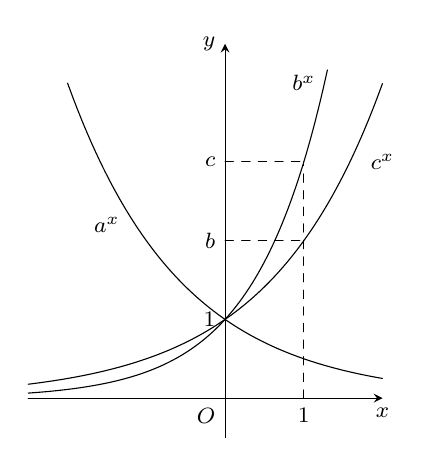
\begin{tikzpicture}[line join = round,line cap = round,>=stealth,font=\footnotesize,scale =1]
		 \draw[->] (-2.5,0) -- (2,0) node[below]{$x$};
		\draw[->] (0,-0.5)  -- (0,4.5) node[left]{$y$};
		 \node at (0,1) [left] {$1$};
		\node at (0,0) [below  left] {$O$};
		\node at (1,0) [below] {$1$}; 
		\node at (0,2) [left] {$b$}; 
		\node  at (0,3) [left] {$c$};
		\draw plot[domain=-2:2,samples=100] (\x,{pow  (0.5,\x)});
		\node at (-1.5,2.2) {$a^x$}; 
		 \draw plot[domain=-2.5:2,samples=100] (\x,{pow (2,\x)});
		\node at  (2,3) {$c^x$};
		\draw  plot[domain=-2.5:1.3,samples=100] (\x,{pow (3,\x)});
		\node at  (1,4) {$b^x$};
		\draw[dashed] (1,0) -- (1,3); 
		 \draw[dashed] (0,2) -- (1,2);
		\draw[dashed] (0,3) -- (1,3); 
	\end{tikzpicture}
		 }
	\loigiai{Dựa vào đồ thị, dễ thấy $\heva{&0<a<1 \\& b, c>1.}$\\ 
		Đường thẳng $x=1$ cắt hai đồ thị $y=b^x$, $y=c^x$ lần lượt tại hai điểm có tung độ  là $b$, $c$ và ta thấy $b>c$.\\
	Vậy $a<c<b$.} 
\end{ex}

% từ: cau-hoi/lop11/1D6_Ham_so_mu_va_ham_so_logarit/1D6-3-3_Su_bien_thien_va_do_thi_cua_ham_so_mu_logarit.tex
\begin{ex}%[1D6H3-3]%[ma:672d10ee]
	 \immini{Đồ thị bên là đồ thị của hàm số nào?
	\choice 
		 {$y=\log_2 x+1$}
		 {$y=\log_2(x+1) $}
		{$y=\log_3  x$}
		{\True $\log_3(x+1) $}}{\begin{tikzpicture}[line join = round,line cap = round,>=stealth,font=\footnotesize,scale =1]
		\draw[->] (-1.7,0) -- (4.2,0) node[below left]  {$x$};
		\draw[->] (0,-1) -- (0,2.5) node[above right]  {$y$};
		\node  at (0,0) [below right] {$O$};
		\node  at (0,1) [left] {$1$};
		\node at  (2,0) [below] {$2$};
		\node at (-1,0)  [below left] {$-1$};
		\draw  (-1,-1) -- (-1,2.5);
		\draw[smooth,domain=-0.65:4] plot (\x,{ln (\x+1)/ln (3)}); 
		\fill  (2,1) circle (1pt);
		 \draw[dashed] (2,1) -- (2,0);
		\draw[dashed]  (2,1) -- (0,1);
	\end{tikzpicture}
		 }
	\loigiai{Đồ  thị hàm số đi qua $(2;1)$, chọn hàm số $y = \log_3(x + 1)$.}
\end{ex}

% từ: cau-hoi/lop11/1D6_Ham_so_mu_va_ham_so_logarit/1D6-3-3_Su_bien_thien_va_do_thi_cua_ham_so_mu_logarit.tex
\begin{ex}%[1D6H3-3]%[ma:3b298901]
	 \immini{
	Đường cong ở  hình bên là đồ thị của hàm số nào
	\choice 
		{$y=2^x$} 
		 {$y=\log_2 x$}
		 {$y=\left(\dfrac{1}{2}\right)^x$}
		{\True $y=\log_{\frac{1}{2}}  x$}
		 }{
		\begin{tikzpicture}[>=stealth,scale=0.7,line join=round,line cap=round]
				\def\xmax{3}  \def\ymin{-1} \def\ymax{2}
				 \draw[->] (-0.5,0)--(\xmax,0) node [below]{$x$};
				 \draw[->] (0,\ymin)--(0,\ymax) node [left]{$y$};
				\node at  (0,0) [below left]{$O$};
				\clip (-0.9,\ymin)  rectangle (\xmax-0.1,\ymax-0.1);
				\draw[smooth,samples=300,domain=0.3:2] plot (\x,{ln(\x)/ln(0.5)}); 
			\end{tikzpicture}
		} 
	\loigiai{Quan sát hình dáng đồ thị ta thấy đồ thị nằm bên phải trục $Oy$, đồ thị  đi xuống từ trái sang phải .
	} 
\end{ex}

% từ: cau-hoi/lop11/1D6_Ham_so_mu_va_ham_so_logarit/1D6-3-3_Su_bien_thien_va_do_thi_cua_ham_so_mu_logarit.tex
\begin{ex}%[1D6H3-3]%[ma:2129bb28]
	Mệnh đề nào trong các  mệnh đề dưới đây \textbf{sai}?
	 \choice
		{Hàm số  $y=\left(\dfrac{2018}{\pi}\right)^x$ đồng biến trên $\mathbb{R}$}
		 {Hàm số $y=\log x$ đồng biến trên $\left(0;+\infty\right)$}
		{\True Hàm số $y=\ln \left(- x\right)$ nghịch biến trên khoảng $\left(-  \infty; 0\right)$}
		{Hàm số $y=2^x$  đồng biến trên $\mathbb{R}$}
	\loigiai{ 
		Hàm số $y=\ln(-x)$ có tập xác  định $\mathscr{D}=\left(- \infty; 0\right)$.\\
		Cơ số $a=\mathrm{e}>1$ do đó hàm số đồng  biến trên $\left(- \infty; 0\right)$.\\
	 }
\end{ex}

% từ: cau-hoi/lop11/1D6_Ham_so_mu_va_ham_so_logarit/1D6-3-3_Su_bien_thien_va_do_thi_cua_ham_so_mu_logarit.tex
\begin{ex}%[1D6V3-3]%[ma:90ccd2b1]
	\immini 
	 {
	Trong hình vẽ bên các đồ thi hàm số $y=\log_ax$, $y=\log_bx$, $y=\log_cx$ với $(0<a, b, c\ne 1)$ cắt các đường thẳng $x=4$, $x=8$ tạo thành hình vuông $MNPQ$ có cạnh bằng $4$. Biết rằng $abc=2^{\tfrac{x}{y}}$ với $x$, $y\in\mathbb{R}^+$ và  $\dfrac{x}{y}$ tối giản, giá trị của $y-x$ bằng
	 \choice
		{$34$} 
		{\True  $5$}
		 {$19$}
		{$43$} 
		 }
		{ 
		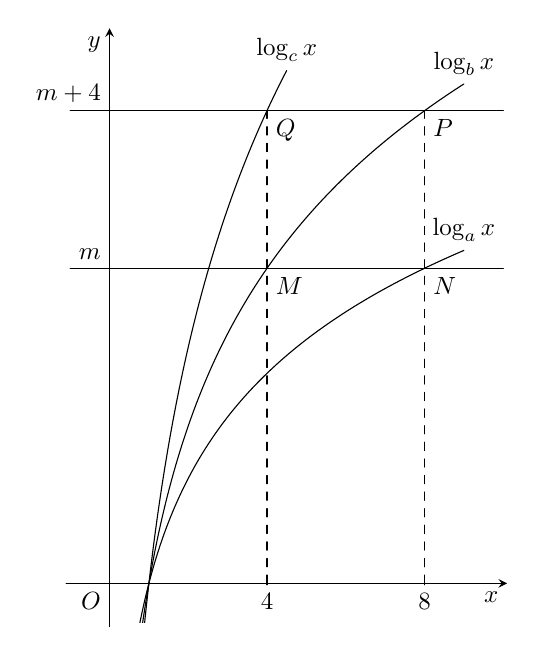
\begin{tikzpicture}[line join=round,line cap=round,>=stealth,scale=0.5]
				\tikzset{every node/.style={scale=0.9}} 
				\draw[->] (-1.1,0)--(10.1,0) node[below left] {$x$}; 
				\draw[->]  (0,-1.1)--(0,14.1) node[below left] {$y$};
				\draw  (0,0) node [below left] {$O$};
				 \foreach \x/\nx in {4/4,8/8}
				\draw[thin]  (\x,1pt)--(\x,-1pt) node [below] {$\nx$};
				\begin{scope}
					\clip (-1,-1) rectangle  (10,14);
					 \draw[samples=200,domain=0.5:9,smooth,variable=\x] plot (\x,{ln((\x))/ln(2^(0.25))}) node[above,sloped]{$\log_bx$};
					\draw[samples=200,domain=0.5:9,smooth,variable=\x] plot (\x,{ln((\x))/ln(2^(0.375))}) node[sloped,above]{$\log_ax$}; 
					 \draw[samples=200,domain=0.5:4.5,smooth,variable=\x] plot (\x,{ln((\x))/ln(2^(0.166667))}) node[above,sloped]{$\log_cx$};
				\end{scope}
				\draw  (-1,8)--(0,8) node[above left]{$m$}--(4,8) node[below right]{$M$}--(8,8) node[below right]{$N$}--(10,8)
					(-1,12)--(0,12) node[above left]{$m+4$}--(4,12) node[below right]{$Q$}--(8,12) node[below  right]{$P$}--(10,12);
				 \draw[dashed]
					 (4,0)--(4,12)
					 (8,0)--(8,12);
			\end{tikzpicture}
		 }
	 \loigiai{
		Hình vuông $MNPQ$ có tọa độ các đỉnh là $M\left(4;\log_b4\right)$, $N\left(8;\log_a8\right)$, $P\left(8;\log_b8\right)$ và  $Q\left(4;\log_c4\right)$.\\
		Ta có $\heva{&\log_c4=\log_b8\\&\log_c4-\log_b4=4}\Rightarrow \log_b8-\log_b4=4\Leftrightarrow \log_b2=4\Leftrightarrow b^4=2\Leftrightarrow b=2^{\tfrac{1}{4}}$.\\ 
		Do $\log_b4=\log_a8$ nên $\log_{2^{\tfrac{1}{4}}}2^2=\log_a8\Leftrightarrow \log_a8=8\Leftrightarrow  a^8=8\Leftrightarrow a=\sqrt[8]{8}=2^{\tfrac{3}{8}}$.\\
		Mà $\log_c4=\log_b8$ nên $\log_c4=\log_{2^{\tfrac{1}{4}}}2^3\Leftrightarrow \log_c4=12\Leftrightarrow c^{12}=4\Leftrightarrow  c=\sqrt[12]{4}=2^{\tfrac{1}{6}}$.\\
		Khi đó  $abc=2^{\tfrac{3}{8}}\cdot 2^{\tfrac{1}{4}}\cdot 2^{\tfrac{1}{6}}=2^{\tfrac{19}{24}}$.\\
		Vậy $x=19$ và $y=24$  nên $y-x=24-19=5$.
	 }
\end{ex}

% từ: cau-hoi/lop11/1D6_Ham_so_mu_va_ham_so_logarit/1D6-3-3_Su_bien_thien_va_do_thi_cua_ham_so_mu_logarit.tex
\begin{ex}%[1D6K3-3]%[ma:06017f90]
	Cho hai hàm số $y=2^x$, $y=\log_2x$ có đồ thị như hình  vẽ. Đường thẳng $\Delta $ cắt trục $Oy$, đồ thị hàm số $y=2^x$, đồ thị hàm số $y=\log_2x$ và trục $Ox$ lần lượt tại $A$, $B$, $C$, $D$ thỏa mãn $AB=BC=CD$. Hỏi có bao nhiêu đường thẳng $\Delta $ như thế?
	\begin{center}
		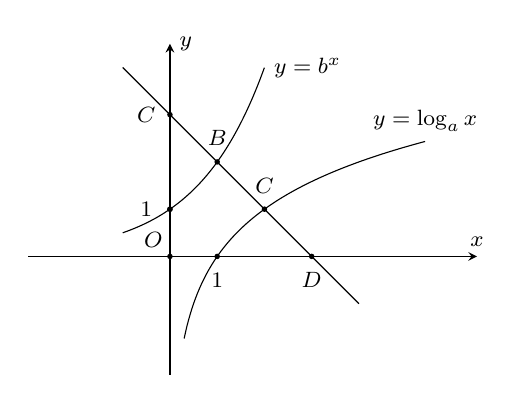
\begin{tikzpicture}[scale=1,>=stealth,font=\footnotesize,line join=round,line cap=roundm,x=0.6cm,y=0.6cm]
				\def  \xmin{-3};
				\def  \xmax{6.5};
				\def  \ymin{-2.5};
				\def  \ymax{4.5};
				\draw[->]  (\xmin,0) -- (\xmax,0) node[above] {$x$};
				 \draw[->] (0.,\ymin) -- (0.,\ymax) node[right] {$y$};
				 \draw[smooth,samples=100,domain=-1:2] plot (\x,{(2^(\x))}) node[right]{$y=b^x$};
				 \draw[smooth,samples=100,domain=0.3:5.4] plot (\x,{(ln(\x))/(ln(2))}) node[above]{$y=\log_ax$};
				 \draw (-1,4)--(4,-1);
				\foreach \x/\y/\l/\g in {0/0/O/135,0/1//0,0/1/1/180,1/0/1/-90,0/3/C/180,3/0/D/-90,2/1/C/90,1/2/B/90}{\fill[black] (\x,\y) circle (1pt)+(\g:0.5) node{$\l$};} 
			\end{tikzpicture}
	\end{center}
	 \choice
		 {\True Vô số đường thẳng $\Delta $}
		 {$2$}
		{$3$} 
		{Không có  đường thẳng nào}
	\loigiai{ 
		Giả sử $A\left(0;3y_0\right)$ và $D\left(3x_0;0\right)$  $\left(x_0,y_0> 0\right)$.\\
		Vì $AB=BC=CD$ nên ta  có $B\left(x_0;2y_0\right)$; $C\left(2x_0;y_0\right)$.\\
		Dễ thấy $B$ và $C$ đối xứng với  nhau qua đường thẳng $y=x$.\\
		Suy ra  $y=x$ chính là đường trung trực của đoạn thẳng $AD$.\\
		Lại do đường thẳng $y=x$ đi qua $O$ nên tam giác $OAD$ là tam giác cân tại $O$.\\ 
		Suy ra  $x_0=y_0$.\\
		 Đặt $x_0=c$. Khi đó $A\left(0;3c\right)$, $D\left(3c;0\right)$.\\
		Đường  thẳng $\Delta $ đi qua $A$ và $D$ có phương trình $y=-x+3c$.\\
		Ta thấy ứng với mỗi giá trị dương của $c$ ta nhận được $4$ điểm $A$,  $B$, $C$, $D$ thỏa mãn yêu cầu bài toán.\\
		Vậy có  vô số đường thẳng $\Delta $.
	} 
\end{ex}

% từ: cau-hoi/lop11/1D6_Ham_so_mu_va_ham_so_logarit/1D6-3-3_Su_bien_thien_va_do_thi_cua_ham_so_mu_logarit.tex
\begin{ex}%[1D6H3-3]%[ma:bf57942c]
	\immini[thm]{Cho $a$, $b$, $c$ là ba số thực dương và khác $1$. Đồ thị các hàm số $y=a^x$, $y=\log_bx$, $y=\log_cx$ được cho trong hình bên. Hãy so  sánh các số thực $a$, $b$, $c$.}
	{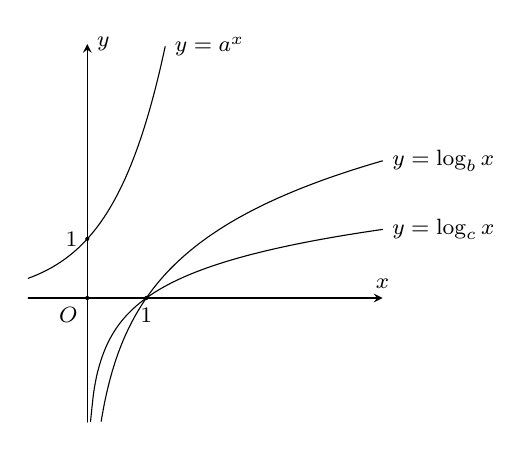
\begin{tikzpicture}[scale=0.75,font=\footnotesize,line join=round,line cap=round,>=stealth]
		 \draw[->](-1,0)--(5,0) node[above]{$x$};
		\draw[->](0,-2.1)--(0,4.3)  node[right]{$y$};
		\draw[smooth,samples=100,domain=-1:1.32]plot (\x,{3^(\x)})  node[right]{$y=a^x$};
		\draw[smooth,samples=100,domain=0.055:5]plot (\x,{ln (\x)/ln  (4)}) node[right]{$y=\log_cx$};
		\draw[smooth,samples=100,domain=0.235:5]plot (\x,{ln (\x)/ln  (2)}) node[right]{$y=\log_bx$};
		 \fill (0,0) node[below left]{$O$}circle (1pt)
			 (1,0) node[below]{$1$}circle (1pt)
			 (0,1) node[left]{$1$}circle (1pt);
	\end{tikzpicture}
	} 
	\loigiai{ 
	 \immini
		 {
		Xét $y=1$, ta  có $\heva{&1=\log_bx\\&1=\log_cx}\Leftrightarrow\heva{&b=x_b\\&c=x_c}\Leftrightarrow x_c>x_b$.\\
		Xét $x=1$, ta lại có $y=a^1=a\Leftrightarrow a=y_a$.\\ 
		Theo  hình vẽ, $x_c>y_a$ và $y_a>x_b$. Vậy $b<a<c$.
		} 
		{ 
		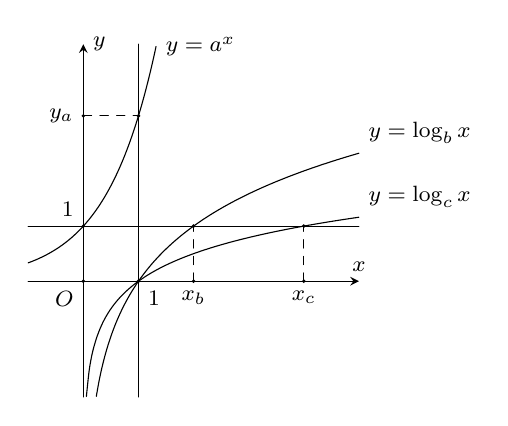
\begin{tikzpicture}[scale=0.7,font=\footnotesize,line join=round,line cap=round,>=stealth]
				\draw[->](-1,0)--(5,0) node[above]{$x$}; 
				\draw[->](0,-2.1)--(0,4.3)  node[right]{$y$};
				\draw[smooth,samples=100,domain=-1:1.32]plot (\x,{3^(\x)})  node[right]{$y=a^x$};
				\draw[smooth,samples=100,domain=0.055:5]plot (\x,{ln  (\x)/ln (4)}) node[above right]{$y=\log_cx$};
				\draw[smooth,samples=100,domain=0.235:5]plot (\x,{ln (\x)/ln (2)})  node[above right]{$y=\log_bx$};
				\fill (2,1) circle (1pt) 
					(4,1)  circle (1pt)
					 (1,3) circle (1pt)
					(0,0) node[below left]{$O$}circle  (1pt)
					(1,0) node[below  right]{$1$}circle (1pt)
					(0,1) node[above left]{$1$}circle (1pt) 
					(0,3)  node[left]{$y_a$}circle (1pt)
					(2,0) node[below]{$x_b$}circle  (1pt)
					 (4,0) node[below]{$x_c$}circle (1pt);
				\draw (-1,1)--(5,1) 
					(1,-2.1)--(1,4.3); 
				 \draw[dashed](2,0)--(2,1)
					 (0,3)--(1,3)
					 (4,0)--(4,1);
			\end{tikzpicture}
		} 
	 }
\end{ex}

% từ: cau-hoi/lop11/1D6_Ham_so_mu_va_ham_so_logarit/1D6-3-3_Su_bien_thien_va_do_thi_cua_ham_so_mu_logarit.tex
\begin{ex}%[1D6H3-3]%[ma:50e38f8a]
	\immini[thm] 
	{ 
	Cho hàm số $y=\log _ax$ ($a>0, a\ne1$) có đồ thị như hình vẽ.  Tìm giá trị của $a$.
	} 
	{ 
	\begin{tikzpicture}[>=stealth,scale=1,line join=round,line cap=round,font=\footnotesize]
			\def\a{1} \def\b{0} \def\c{-3} \def\d{1} 
			\def\xt{-1}  \def\xp{3} \def\yt{3} \def\yd{-1.5}
			\draw[fill] (1,0) circle (1pt)  node[below]{$1$}
				 (0,-1) circle (1pt) node[left]{$-1$}
				 (0,1) circle (1pt) node[left]{$1$}
				(2,0) circle  (1pt) node[above]{$2$};
			\draw[->] (\xt,0)--(\xp,0) node  [below]{$x$};
			\draw[->]  (0,\yd)--(0,\yt) node [left]{$y$};
			 \node at (0,0) [below right]{$O$};
			\clip (\xt-0.1,\yd+0.1) rectangle  (\xp-0.1,\yt-0.1);
			\draw[smooth,domain=0.1:3] plot (\x,{ln (\x)/(ln (0.5))}); 
			\draw[dashed]  (2,0)|-(0,-1);
		\end{tikzpicture}
	 }
	\loigiai{ 
		Đồ thị hàm số  $y=\log_ax$ đi qua điểm $(2;-1)$ nên $\log_a2=-1$.\\
		Khi đó $a^{-1}=2  \Leftrightarrow \dfrac{1}{a}=2 \Leftrightarrow a=\dfrac{1}{2}$.
	 }
\end{ex}

% từ: cau-hoi/lop11/1D6_Ham_so_mu_va_ham_so_logarit/1D6-3-3_Su_bien_thien_va_do_thi_cua_ham_so_mu_logarit.tex
\begin{bt}%[1D6H3-3]%[ma:d831a67c]
% nguon: Archive/2024/TOAN_11_XE/TOAN_11_XE/data4/11C6/KNTT-6.3.tex #1005
%[Đỗ Minh Phúc]
	Lập bảng biến thiên và vẽ đồ thị hàm số
	\begin{multicols}{2}
		\begin{enumerate}
			\item $y=4^x$;
			\item $y=\log_{\tfrac{1}{4}} x$.
		\end{enumerate}
	\end{multicols}
	\loigiai{
		\begin{enumerate}
			\item 	Vì hàm số $y=4^x$ có cơ số $4>1$ nên ta có bảng biến thiên như sau
			\begin{center}
				
\begin{tikzpicture}[>=stealth,line join=round,line cap=round,font=\footnotesize,scale=1]
					\tkzTabInit[nocadre=false,lgt=2,espcl=2,deltacl=0.5]{$x$/0.7,$y=4^x$/2}
					{$-\infty$ , $0$ , $+\infty$}
					\tkzTabVar{-/$0$ , R , +/$+\infty$}
					\tkzTabIma{1}{3}{2}{$1$}% Từ cột 1 đến cột 3 đặt f(2) tại cột 2.
				\end{tikzpicture}
			\end{center}
			Đồ thị của hàm số $y=4^x$ là một đường cong liền nét đi qua các điểm $A\left(-1;\dfrac{1}{4}\right)$, $B(0;1)$, $C(1;4)$, $D(2;16)$.
			\begin{center}
				\begin{tikzpicture}[>=stealth,line join=round,line cap=round,font=\footnotesize,scale=0.8,yscale=0.7]
					\def\a{4}
					\draw[->] (-3.5,0) -- (5,0) node[below] {$x$};
					\draw[->] (0,-2) -- (0,17) node[left] {$y$};
					\draw (0,0)node[below right=-0.05]{$O$};
					\clip (-5,-5)rectangle(5,16.5);
					\draw[thick,samples=200,smooth,domain=-3:4] plot(\x, {\a^\x});
					\draw[dashed] (0,4)--(1,4) node[right]{$C$}--(1,0);
					\draw[dashed] (0,16)--(2,16)node[right]{$D$}--(2,0);
					\draw[dashed] (-1,0)--(-1,1/4)node[above left]{$A$}--(0,1/4)node[right]{$\frac{1}{4}$};
					\draw (0,1) node [above left=-0.1] {$1$}node[right]{$B$};
					\draw (1,0) node [below] {$1$};
					\draw (0,4) node [left] {$4$};
					\draw (2,0) node [below] {$2$};
					\draw (0,16) node [left] {$16$};
					\draw (-1,0) node [below] {$-1$};
				\end{tikzpicture}
			\end{center}
			\item Vì hàm số $y=\log_{\tfrac{1}{4}} x$ có cơ số $\dfrac{1}{4}<1$ nên ta có bảng biến thiên như sau
			\begin{center}
				
\begin{tikzpicture}[>=stealth,line join=round,line cap=round,font=\footnotesize,scale=1]
					\tkzTabInit[nocadre=true,lgt=2.3,espcl=2,deltacl=0.5]{$x$/0.7,$y=\log_{\tfrac{1}{4}}x$/2}
					{$0$ , $1$ , $+\infty$}
					\tkzTabVar{+/$+\infty$ , R , -/$-\infty$}
					\tkzTabIma{1}{3}{2}{$0$}% Từ cột 1 đến cột 3 đặt f(2) tại cột 2.
				\end{tikzpicture}
			\end{center}
			Đồ thị của hàm số $y=\log_{\tfrac{1}{4}}x$ là một đường cong liền nét đi qua các điểm $A\left(\dfrac{1}{4};1\right)$, $B(1;0)$, $C(4;-1)$, $D(16;-2)$.
			\begin{center}
				\begin{tikzpicture}[>=stealth,line join=round,line cap=round,font=\footnotesize,scale=0.9,xscale=0.8]
					\draw[->](-1,0) -- (17,0) node[below]{ $x$};
					\draw[->](0,-3) -- (0,4) node[below,right]{ $y$};
					\draw(-0.2,0) node[below left]{\footnotesize $O$};
					\clip(-2,-3) rectangle (17,4);
					\draw[smooth,samples=300,domain=0.03:16.5]plot(\x,{ln(\x)/ln(0.25)});
					\draw(1,0) node[below]{$1$}node[above]{$B$};
					\draw[dashed] (0,-1) node[left]{$-1$}--(4,-1)node[below]{$C$}--(4,0)node[above]{$4$};
					\draw[dashed] (0,-2) node[left]{$-2$}--(16,-2)node[below]{$D$}--(16,0)node[above]{$16$};
					\draw[dashed] (0,1) node[left]{$1$}--(1/4,1)node[right]{$A$}--(1/4,0)node[below]{$\frac{1}{4}$};
					\draw (0.1,2)node[right]{$y=\log_{\tfrac{1}{4}}x$};
				\end{tikzpicture}
			\end{center}
		\end{enumerate}
	}	
\end{bt}

% từ: cau-hoi/lop11/1D6_Ham_so_mu_va_ham_so_logarit/1D6-3-5_Toan_thuc_te_ap_dung_ham_so_mu_logarit.tex
\begin{bt}%[1D6C3-5]%[ma:b07438f5]
	Người ta xây dựng một cây cầu vượt giao thông hình parabol nối hai điểm có khoảng cách  là $400$m. Độ dốc của mặt cầu không vượt quá $10^{\circ}$ (độ dốc tại một điểm được xác định bởi góc giữa phương tiếp xúc với mặt cầu và phương ngang). Tính chiều cao giới hạn từ đỉnh cầu đến mặt đường (làm tròn kết quả đến chữ số thập phân thứ nhất).
	\begin{center}
		\begin{tikzpicture}[>=latex,line join=round,line cap=round,scale=1]
				\coordinate (M)  at (-1.5,1);
				 \coordinate (P) at (-3,1);
				\coordinate (N)  at (1,4);
				\draw[samples=200,smooth,red,line width=1] plot[domain=-4:4] (\x,{sqrt  (25-(\x)^2)-3})--(-4,0);
				\draw[samples=200,smooth,blue,line width=1]  plot[domain=-4:-1] (\x,{(3*(\x)+13)/4});
				\draw[dashed] (-4,0)  node[below]{$A$}
					(4,0)  node[below]{$B$}
					(0,0) node[below]{$400$m}--(0,1)  node[right]{?}--(0,2)
					(P)  node[above]{$P$}--(M);
				 \draw pic["",draw=blue,-,angle eccentricity=1.2,angle radius=0.4cm] {angle=M--P--N};
			\end{tikzpicture}
	\end{center}
	 \loigiai{
		Chọn hệ  trục toạ độ như hình vẽ, sao cho đỉnh cầu là gốc tọa độ và mặt cắt của cây cầu có hình dạng parabol $y=-ax^2$ (với $a$ là hằng số dương).
		\begin{center}
			\begin{tikzpicture}[>=latex,line join=round,line cap=round,scale=1]
					\draw[->]  (-5,2)--(5,2) node[above]{$x$};
					\draw[->] (0,-1)--(0,3)  node[right]{$y$};
					\coordinate  (M) at (-1.5,1);
					\coordinate (P) at  (-3,1);
					\coordinate (N) at (1,4); 
					 \draw[dashed] (-4,2) node[above]{$-200$}|-(0,0) node[below right]{$I$}-|(4,2) node[above]{$200$};
					\draw[samples=200,smooth,red,line width=1] plot[domain=-4:4] (\x,{sqrt  (25-(\x)^2)-3})--(-4,0);
					\draw[samples=200,smooth,blue,line  width=1] plot[domain=-4:-1] (\x,{(3*(\x)+13)/4});
					\draw[dashed] (-4,0) node[below]{$A$} 
						(4,0)  node[below]{$B$}
						(0,0)--(0,1)  node[right]{?}--(0,2)
						(P) node[above]{$P$}--(M); 
					\draw  pic["",draw=blue,-,angle eccentricity=1.2,angle radius=0.4cm] {angle=M--P--N};
				\end{tikzpicture}
		\end{center}
		Hệ số góc của tiếp tuyến của parabol  bằng $k=y^{\prime}\left(x_0\right)=-2ax_0$, $-200\leq x_0\leq200$.\\
		Hệ số góc xác định độ dốc của mặt cầu (độ dốc dương)  là $|k|=2a|x|\leq400a$.\\
		Vì độ dốc của mặt cầu không  vượt quá $10^{\circ}$ nên ta có:
		$400a\leq\tan10^{\circ}\Leftrightarrow  a\leq\dfrac{4,408174518}{10000}$.\\
		Chiều cao giới hạn từ đỉnh cầu đến mặt đường là đoạn $OI$, cũng chính là độ  lớn của tung độ điểm $B$ khi $a$ đạt giá trị lớn nhất.\\
		Do đó, $OI=\left|-a\cdot200^2\right|=17,6$  (m).\\
		Vậy chiều cao giới hạn từ đỉnh cầu đến mặt đường là $17,6$ m. 
	} 
\end{bt}

% từ: cau-hoi/lop11/1D6_Ham_so_mu_va_ham_so_logarit/1D6-3-5_Toan_thuc_te_ap_dung_ham_so_mu_logarit.tex
\begin{ex}%[1D6C3-5]%[ma:5e0be94c]
	Người ta xây dựng một cây cầu vượt giao thông hình parabol nối hai điểm có khoảng cách là $400$m. Độ dốc của mặt cầu không vượt quá $10^{\circ}$ (độ dốc tại một điểm được xác định bởi góc giữa phương tiếp xúc với mặt cầu và phương ngang). Tính chiều cao giới hạn từ đỉnh cầu  đến mặt đường (làm tròn kết quả đến chữ số thập phân thứ nhất).
	\begin{center}
		\begin{tikzpicture}[>=latex,line join=round,line cap=round,scale=1]
				\coordinate (M)  at (-1.5,1);
				 \coordinate (P) at (-3,1);
				\coordinate (N) at (1,4); 
				\draw[samples=200,smooth,red,line  width=1] plot[domain=-4:4] (\x,{sqrt (25-(\x)^2)-3})--(-4,0);
				\draw[samples=200,smooth,blue,line  width=1] plot[domain=-4:-1] (\x,{(3*(\x)+13)/4});
				 \draw[dashed] (-4,0) node[below]{$A$}
					 (4,0) node[below]{$B$}
					(0,0)  node[below]{$400$m}--(0,1) node[right]{?}--(0,2)
					(P) node[above]{$P$}--(M); 
				 \draw pic["",draw=blue,-,angle eccentricity=1.2,angle radius=0.4cm] {angle=M--P--N};
			\end{tikzpicture}
	\end{center}
	 \loigiai{
		Chọn hệ trục toạ độ như hình vẽ, sao cho đỉnh cầu là gốc tọa  độ và mặt cắt của cây cầu có hình dạng parabol $y=-ax^2$ (với $a$ là hằng số dương).
		\begin{center}
			\begin{tikzpicture}[>=latex,line join=round,line cap=round,scale=1]
					\draw[->] (-5,2)--(5,2)  node[above]{$x$};
					\draw[->] (0,-1)--(0,3) node[right]{$y$}; 
					\coordinate  (M) at (-1.5,1);
					\coordinate  (P) at (-3,1);
					\coordinate (N) at  (1,4);
					\draw[dashed] (-4,2) node[above]{$-200$}|-(0,0)  node[below right]{$I$}-|(4,2) node[above]{$200$};
					\draw[samples=200,smooth,red,line  width=1] plot[domain=-4:4] (\x,{sqrt (25-(\x)^2)-3})--(-4,0);
					\draw[samples=200,smooth,blue,line width=1] plot[domain=-4:-1]  (\x,{(3*(\x)+13)/4});
					\draw[dashed] (-4,0)  node[below]{$A$}
						 (4,0) node[below]{$B$}
						(0,0)--(0,1) node[right]{?}--(0,2) 
						(P)  node[above]{$P$}--(M);
					\draw pic["",draw=blue,-,angle  eccentricity=1.2,angle radius=0.4cm] {angle=M--P--N};
				\end{tikzpicture}
		\end{center}
		Hệ số góc của tiếp tuyến của parabol bằng $k=y^{\prime}\left(x_0\right)=-2ax_0$, $-200\leq  x_0\leq200$.\\
		Hệ số góc xác định độ dốc của mặt  cầu (độ dốc dương) là $|k|=2a|x|\leq400a$.\\
		Vì độ  dốc của mặt cầu không vượt quá $10^{\circ}$ nên ta có:
		 $400a\leq\tan10^{\circ}\Leftrightarrow a\leq\dfrac{4,408174518}{10000}$.\\
		Chiều cao giới  hạn từ đỉnh cầu đến mặt đường là đoạn $OI$, cũng chính là độ lớn của tung độ điểm $B$ khi $a$ đạt giá trị lớn nhất.\\
		 Do đó, $OI=\left|-a\cdot200^2\right|=17,6$ (m).\\
		 Vậy chiều cao giới hạn từ đỉnh cầu đến mặt đường là $17,6$ m.
	 }
\end{ex}

% từ: cau-hoi/lop11/1D6_Ham_so_mu_va_ham_so_logarit/1D6-4-2_Phuong_trinh_mu_logarit_co_ban.tex
\begin{bt}%[1D6H4-2]%[ma:64cad100]
	Giải các phương trình  sau:
	\begin{multicols}{2}
		\begin{enumerate}
			\item  $4^x-2^{x+2}-3=0$;
			\item $9^x-5\cdot  3^x+6=0$;
			\item $4\cdot 4^x-9\cdot  2^{x+1}+8=0$;
			\item $2^{2x+1}+15\cdot  2^x-8=0$.
		\end{enumerate}
	\end{multicols}
	\loigiai{ 
		\begin{enumerate}
			\item Ta có  $4^x-2^{x+2}-3=0 \Leftrightarrow \left(2^x\right)^2-2^x \cdot 2^2 -3=0 \Leftrightarrow \left(2^x\right)^2-4\cdot 2^x-3=0$. \qquad ($1$)\\
			Đặt $t=2^x$, $t>0$. Khi đó phương trình  ($1$) trở thành\\
			$t^2-4t-3=0 \Leftrightarrow \hoac{&t=2-\sqrt{7}\\&t=2+\sqrt{7}}\Leftrightarrow  t=2+\sqrt{7}$.\\
			 Với $t=2+\sqrt{7} \Rightarrow 2^x=2+\sqrt{7} \Leftrightarrow x=\log_2 \left(2+\sqrt{7}\right)$.\\
			Vậy phương trình có  một nghiệm $x=\log_2 \left(2+\sqrt{7}\right)$
			\item Ta có $9^x-5\cdot 3^x+6=0 \Leftrightarrow \left(3^x\right)^2-5\cdot 3^x+6=0$. \qquad  ($2$)\\
			Đặt $t=3^x$, $t>0$. Khi đó phương trình ($2$)  trở thành $t^2-5t+6=0 \Leftrightarrow \hoac{&t=2\\&t=3.}$\\
			Với $t=2 \Rightarrow 3^x=2  \Leftrightarrow x=\log_3 2$.\\
			Với $t=3 \Leftrightarrow 3^x=3 \Leftrightarrow  x=1$.\\
			Vậy phương trình có hai  nghiệm $x=\log_3 2$, $x=1$
			\item Ta có $4\cdot 4^x-9\cdot 2^{x+1}+8=0 \Leftrightarrow 4\cdot \left(2^x\right)^2-18\cdot 2^x+8=0$.  \qquad ($3$)\\
			Đặt $t=2^x$, $t>0$.  Khi đó phương trình ($3$) trở thành $4t^2-18t+8=0 \Leftrightarrow \hoac{&t=4\\&t=\dfrac{1}{2}.}$\\
			Với $t=4 \Leftrightarrow  2^x=4 \Leftrightarrow x=2$.\\
			Với $t=\dfrac{1}{4}  \Leftrightarrow 2^x=\dfrac{1}{4}\Leftrightarrow x=-2$.\\
			Vậy phương trình có hai nghiệm  $x=2$, $x=-2$.
			\item Ta có $2^{2x+1}+15\cdot 2^x-8=0 \Leftrightarrow 2\cdot \left(2^x\right)^2+15\cdot 2^x-8=0$. \qquad  ($4$)\\
			Đặt $t=2^x$, $t>0$. Khi đó phương trình ($4$) trở thành 
			\begin{center}
				$2t^2+15t-8=0 \Leftrightarrow \hoac{&t=\dfrac{1}{2}\\&t=-8}\Leftrightarrow  t=\dfrac{1}{2}.$
			\end{center}
			Với $t=\dfrac{1}{2} \Leftrightarrow 2^x=\dfrac{1}{2}\Leftrightarrow x=-1$.\\ 
			Vậy phương trình có một nghiệm $x=-1$ 
		\end{enumerate}
	} 
\end{bt}

% từ: cau-hoi/lop11/1D6_Ham_so_mu_va_ham_so_logarit/1D6-4-2_Phuong_trinh_mu_logarit_co_ban.tex
\begin{ex}%[1D6H4-2]%[ma:95463e99]
	Giải  các phương trình sau
	\begin{multicols}{3}
		\begin{enumerate}
			 \item $2^{2x-1}-\dfrac{1}{8}=0$;
			\item $2^{(x-1)^2}=4^x$; 
			\item $25^x=5^{x^2}$; 
			\item  $\left(\dfrac{1}{25}\right)^{x+1}=125^x$;
			 \item $\left(\dfrac{1}{4}\right)^{2x-1}=\left(2\sqrt{2}\right)^{x+2}$;
			 \item $4^{x^2-2x}=1$.
		\end{enumerate}
	\end{multicols}
	 \loigiai{
		\begin{enumerate}
			\item $2^{2x-1}-\dfrac{1}{8}=0 \Leftrightarrow 2^{2x-1}=2^{-3}\Leftrightarrow  2x-1=-3\Leftrightarrow x=-1$.
			 \item $2^{(x-1)^2}=4^x \Leftrightarrow 2^{(x-1)^2}=2^{2x}\Leftrightarrow (x-1)^2=2x\Leftrightarrow x^2-4x+1=0\Leftrightarrow \hoac{&x=2+\sqrt{3}\\&x=2-\sqrt{3}.}$
			\item $25^x=5^{x^2}\Leftrightarrow 5^{2x}=5^{x^2}\Leftrightarrow  2x=x^2\Leftrightarrow \hoac{&x=0\\&x=2.}$
			\item  $\left(\dfrac{1}{25}\right)^{x+1}=125^x \Leftrightarrow 5^{-2(x+1)}=5^{3x}\Leftrightarrow -2(x+1)=3x \Leftrightarrow x=-\dfrac{2}{5}$.
			 \item
			\begin{eqnarray*} &&\left(\dfrac{1}{4}\right)^{2x-1}=\left(2\sqrt{2}\right)^{x+2}\\
				&\Leftrightarrow& \left(2^{-2}\right)^{2x-1}=\left(2\cdot 2^{\tfrac{1}{2}}\right)^{x+2}\\ 
				&\Leftrightarrow&  2^{-4x+2}=2^{\tfrac{3(x+2)}{2}} \\
				&\Leftrightarrow&  -4x+2=\dfrac{3(x+2)}{2} \\
				&\Leftrightarrow& x=-\dfrac{2}{11}. 
			\end{eqnarray*}
			\item $4^{x^2-2x}=1 \Leftrightarrow  x^2-2x=0 \Leftrightarrow \hoac{&x=0\\&x=2.}$
		\end{enumerate}
	 }
\end{ex}

% từ: cau-hoi/lop11/1D6_Ham_so_mu_va_ham_so_logarit/1D6-4-3_Bat_phuong_trinh_mu_logarit_co_ban.tex
\begin{bt}%[1D6H4-3]%[ma:1585b909]
	Giải bất phương trình sau  $5^{\left|x^2-2 x\right|}>125$
	 \loigiai{ \\
		$5^{\left|x^2-2 x\right|}>125  \Leftrightarrow\left|x^2-2 x\right|>\log _5 125 \Leftrightarrow\left|x^2-2 x\right|>3 \Leftrightarrow \hoac{&x^2-2x>3 \\ &x^2-2x<-3} \Leftrightarrow \hoac{& x<-1 \\ & x>3.}$ \\
		Tập nghiệm $\mathrm{S}=(-\infty;-1)  \cup(3;+\infty)$
	 }
\end{bt}

% từ: cau-hoi/lop11/1D6_Ham_so_mu_va_ham_so_logarit/1D6-4-4_Phuong_trinh_mu_logarit_dua_ve_cung_co_so.tex
\begin{ex}%[1D6V4-4]%[ma:46b50b8a]
  Cho phương trình $\log_2 \left(x^2-x+2\right)=1$.
 \choiceTF 
  {Điều kiện xác  định của phương trình là $x > 0$}
  {\True Phương trình  có hai nghiệm phân biệt}
  {\True Tổng bình phương các nghiệm  là $1$}
  {Phương  trình có hai nghiệm trái dấu}
  \loigiai{
  \begin{itemchoice}
   \itemch Sai. Điều kiện xác định của phương trình là $x^2-x+2> 0\Leftrightarrow  \forall x\in \mathbb{R}$.
    \itemch Đúng. $\log_2\left(x^2-x+2\right)=1\Leftrightarrow x^2-x+2=2\Leftrightarrow \hoac{&{x=0} \\
    &{x=1.}
    &}$
   \itemch  Đúng. Tổng bình phương các nghiệm là $0^2+1^2=1$.
   \itemch Sai. Phương trình có hai nghiệm phân  biệt $x=0$ và $x=1$.
  \end{itemchoice}
  }
\end{ex}

% từ: cau-hoi/lop11/1D7_Dao_ham/1D7-1-4_Y_nghia_Vat_ly_cua_dao_ham.tex
\begin{ex}%[1D7N1-4]%[ma:730dcfa5]
	Cho chuyển động xác định bởi phương trình $S=t^3-3t^2-9t$, trong đó $t$ được tính bằng giây và $S$ được tính bằng mét. Tính vận tốc của chuyển động tại thời điểm gia tốc triệt  tiêu.
	 \choice
		{$3$  m/s}
		{\True  $-12$ m/s}
		{$12$  m/s}
		{$-3$  m/s}
	\loigiai{Gia tốc  của chuyển động là $a(t)=S''(t)=6t-6.$\\
		Gia tốc triệt tiêu khi $a(t)=0\Leftrightarrow t=1.$\\ 
		 Vận tốc tại thời điểm gia tốc triệt tiêu là $v(1)=S'(1)=-12$ m/s.
	} 
\end{ex}

% từ: cau-hoi/lop11/1D7_Dao_ham/1D7-1-4_Y_nghia_Vat_ly_cua_dao_ham.tex
\begin{bt}%[1D7H1-4]%[ma:68062199]
	Một chất điểm chuyển động theo phương trình $s(t)=3 \sin 2 t+2 \cos 2 t$, trong đó $t$ là thời gian tính bằng giây và $s(t)$ là quãng đường chuyển động được của chất điểm trong $t$ giây tính bằng mét. Tính gia tốc của chất điểm đó khi  $t=\dfrac{\pi}{4}$.
	 \loigiai{ \\
		Ta có $s'(t)=3(\sin 2 t)'+2(\cos 2  t)'=6 \cos 2 t-4 \sin 2 t$.\\
		Và $s''(t)=6(\cos 2 t)'-4(\sin 2 t)'=-12 \sin 2 t-8 \cos  2 t$.\\
		Gia tốc  của chất điểm tại thời điểm $t=\dfrac{\pi}{4}$ là \\
		$a\left(\dfrac{\pi}{4}\right)=s'' \left(\dfrac{\pi}{4}\right)=-12\left[\sin  \left(2 \cdot \dfrac{\pi}{4}\right)\right]-8\left[\cos \left(2 \cdot \dfrac{\pi}{4}\right)\right]=-12$.
	} 
\end{bt}

% từ: cau-hoi/lop11/1D7_Dao_ham/1D7-1-4_Y_nghia_Vat_ly_cua_dao_ham.tex
\begin{ex}%[1D7H1-4]%[ma:efdcdbae]
	Một chất điểm chuyển động  theo phương trình $s(t)=3 \sin 2 t+2 \cos 2 t$, trong đó $t$ là thời gian tính bằng giây và $s(t)$ là quãng đường chuyển động được của chất điểm trong $t$ giây tính bằng mét. Tính gia tốc của chất điểm đó khi $t=\dfrac{\pi}{4}$.
	\loigiai{ \\ 
		Ta có $s'(t)=3(\sin 2 t)'+2(\cos 2 t)'=6 \cos 2  t-4 \sin 2 t$.\\
		Và  $s''(t)=6(\cos 2 t)'-4(\sin 2 t)'=-12 \sin 2 t-8 \cos 2 t$.\\
		Gia tốc của chất điểm tại thời điểm $t=\dfrac{\pi}{4}$ là \\ 
		$a\left(\dfrac{\pi}{4}\right)=s'' \left(\dfrac{\pi}{4}\right)=-12\left[\sin \left(2 \cdot \dfrac{\pi}{4}\right)\right]-8\left[\cos  \left(2 \cdot \dfrac{\pi}{4}\right)\right]=-12$.
	 }
\end{ex}

% từ: cau-hoi/lop11/1D7_Dao_ham/1D7-1-4_Y_nghia_Vat_ly_cua_dao_ham.tex
\begin{bt}%[1D7H1-4]%[ma:9fa0033b]
% nguon: Archive/SP_KhoLatex/ID6_old/16-OT-DaoHam-CongThucTinhDaoHam.tex #3830
%[ĐGNL, Nguyễn Thành Nhân]
	Cho chuyển động thẳng xác định bởi phương trình $s(t)=t^3+3t^2-9t+27$, trong đó $t$ tính bằng giây (s) và $S$ được tính bằng mét (m). Tính gia tốc của chuyển động tại thời điểm vận tốc triệu tiêu.
\loigiai{
		$v(t)=s'(t)=3t^2+6t-9$, $a(t)=v'(t)=6t+6$\\
		Thời điểm vận tốc triệt tiêu $v(t)=0\Leftrightarrow 3t^2+6t-9=0\Leftrightarrow \hoac {&t=-3\quad \text {loại do }t>0\\&t=1}$\\
		Gia tốc cần tìm $a(1)=12$ m/s$^2$.}
\end{bt}

% từ: cau-hoi/lop11/1D7_Dao_ham/1D7-1-5_Toan_thuc_te_khac_ap_dung_dinh_nghia_dao_ham.tex
\begin{ex}%[1D7V1-5]%[ma:25db80be]
	Cho chuyển động thẳng xác định bởi phương trình $S=-t^3+3 t^2+9 t$,  trong đó $t$ tính bằng giây và $S$ tính bằng mét. Tính vận tốc của chuyển động tại thời điểm gia tốc triệt tiêu.\\
	\shortans{12} 
	 \loigiai{
		Ta có: $v=S^{\prime}=-3 t^2+6 t+9$ và $a=v^{\prime}=-6 t+6$.\\ 
		Gia tốc triệt tiêu khi $a=0\Rightarrow  t=1$.\\
		Khi đó vận tốc của  chuyển động là $v(1)=12$ m/s.
	 }
\end{ex}

% từ: cau-hoi/lop11/1D7_Dao_ham/1D7-2-1_Tinh_dao_ham.tex
\begin{bt}%[1D7H2-1]%[ma:e0a37dab]
% nguon: Archive/2024/TOAN_11_XE/TOAN_11_XE/data4/11C9/KNTT-9.OTC.tex #1346
%[TeX hóa SGK11]%[Lê Quang Xe]
	Tìm đạo hàm của mỗi hàm số sau:
	\begin{listEX}[3]
		\item[a)] $y=\left(x^2+2 x\right)\left(x^3-3 x\right)$;
		\item[b)] $y=\dfrac{1}{-2 x+5}$;
		\item[c)] $y=\sqrt{4 x+5}$;
		\item[d)] $y=\sin x \cos x$;
		\item[e)] $y=x \mathrm{e}^x$;
		\item[f)] $y=\ln ^2 x$.
	\end{listEX}
	\loigiai{
		\begin{listEX}
			\item[a)] Ta có 
			\allowdisplaybreaks
			\begin{eqnarray*}
				y'&=&\left(x^2+2 x\right)'\left(x^3-3 x\right)+\left(x^2+2 x\right)\left(x^3-3 x\right)'\\
				&=&\left(2x+2\right)\left(x^3-3 x\right)+\left(x^2+2 x\right)\left(3x^2-3\right)\\
				&=&5x^4+8x^3-9x^2-12x.
			\end{eqnarray*}	
			Vậy $y'=5x^4+8x^3-9x^2-12x$.
			\item[b)] Ta có 
			\allowdisplaybreaks
			\begin{eqnarray*}
				y'&=&\dfrac{-(-2x+5)'}{(-2x+5)^2}\\
				&=&\dfrac{2}{(-2x+5)^2}.
			\end{eqnarray*}
			Vậy $y'=\dfrac{2}{(-2x+5)^2}$.
			\item[c)] Ta có 
			\allowdisplaybreaks
			\begin{eqnarray*}
				y'&=&\dfrac{(4x+5)'}{2\sqrt{4x+5}}\\
				&=&\dfrac{2}{\sqrt{4x+5}}.
			\end{eqnarray*}
			Vậy $y'=\dfrac{2}{\sqrt{4x+5}}$.
			\item[d)] Ta có 
			\allowdisplaybreaks
			\begin{eqnarray*}
				y'&=&\left( \sin x\right)'  \cdot \cos x + \sin x \cdot \left( \cos x\right) '\\
				&=& \cos x \cdot \cos x + \sin x \cdot \left( -\sin x \right) \\
				&=&\cos2x.
			\end{eqnarray*}
			Vậy $y'=\cos2x$.
			\item[e)] Ta có 
			\allowdisplaybreaks
			\begin{eqnarray*}
				y'&=&\left( x\right)' \cdot \mathrm{e}^x + x \cdot \left( \mathrm{e}^x\right) '\\
				&=& \mathrm{e}^x + x \cdot \mathrm{e}^x \\
				&=&\left( 1+x\right) \mathrm{e}^x.
			\end{eqnarray*}
			Vậy $y'=\left( 1+x\right) \mathrm{e}^x.$
			\item[f)] Ta có 
			\allowdisplaybreaks
			\begin{eqnarray*}
				y'&=&2\cdot \ln x \cdot \left(\ln x \right)' \\
				&=& \dfrac{2 \ln x}{x}.
			\end{eqnarray*}
			Vậy $y'=\dfrac{2 \ln x}{x}.$
	\end{listEX}}
\end{bt}

% từ: cau-hoi/lop11/1D7_Dao_ham/1D7-2-8_Toan_thuc_te_ap_dung_quy_tac_dao_ham.tex
\begin{bt}%[1D7C2-8]%[ma:493ee940]
	Một con lắc lò xo dao động điều hoà theo phương ngang trên mặt phẳng không ma sát, có phương trình chuyển động $x=4\cos \left(\pi t-\dfrac{2\pi}{3}\right)+4$ (cm), trong đó $t$ là thời gian tính bằng giây. Tìm thời điểm mà vận tốc tức thời của con lắc bằng $0$  (cm/s).
	\loigiai{ 
		Ta có $v(t)=x^{\prime}=-4\pi \sin \left(\pi t-\dfrac{2\pi}{3}\right)$.  \\
		Thời điểm mà vận tốc tức thời của con lắc  bằng $0$ nghĩa là
		\begin{eqnarray*}
			 & & v(t)=0 \\
			& \Leftrightarrow& -4 \pi \sin \left(\pi t-\dfrac{2 \pi}{3}\right)=0  \\
			 &\Leftrightarrow& \sin \left(\pi t-\dfrac{2 \pi}{3}\right)=0 \\
			&\Leftrightarrow& \pi t-\dfrac{2 \pi}{3}=k \pi \\ 
			&\Leftrightarrow& t=\dfrac{2}{3}+k \quad  (k \in \mathbb{Z}).
		\end{eqnarray*}
		Vậy các thời điểm mà vận tốc tức thời của con lắc  bằng $0$ là
		$$ 
		t=\dfrac{2}{3}+k \text{ (s)} \quad (k \in \mathbb{Z}) 
		$$ 
	 }
\end{bt}

% từ: cau-hoi/lop11/1D7_Dao_ham/1D7-2-8_Toan_thuc_te_ap_dung_quy_tac_dao_ham.tex
\begin{ex}%[1D7C2-8]%[ma:b29b0369]
	Một con lắc lò xo dao động điều hoà theo phương ngang trên mặt phẳng không ma sát, có phương trình chuyển động $x=4\cos \left(\pi t-\dfrac{2\pi}{3}\right)+4$ (cm), trong đó $t$ là thời gian tính bằng giây. Tìm thời điểm  mà vận tốc tức thời của con lắc bằng $0$ (cm/s).
	 \loigiai{
		Ta có $v(t)=x^{\prime}=-4\pi  \sin \left(\pi t-\dfrac{2\pi}{3}\right)$. \\
		Thời điểm mà vận tốc tức thời của con  lắc bằng $0$ nghĩa là
		\begin{eqnarray*}
			& & v(t)=0  \\
			& \Leftrightarrow& -4 \pi \sin \left(\pi t-\dfrac{2 \pi}{3}\right)=0  \\
			&\Leftrightarrow& \sin  \left(\pi t-\dfrac{2 \pi}{3}\right)=0 \\
			&\Leftrightarrow& \pi  t-\dfrac{2 \pi}{3}=k \pi \\
			&\Leftrightarrow&  t=\dfrac{2}{3}+k \quad (k \in \mathbb{Z}).
		\end{eqnarray*}
		Vậy các thời điểm mà vận tốc tức thời của con lắc  bằng $0$ là
		$$ 
		 t=\dfrac{2}{3}+k \text{ (s)} \quad (k \in \mathbb{Z})
		$$ 
	} 
\end{ex}

% từ: cau-hoi/lop11/1D7_Dao_ham/1D7-2-8_Toan_thuc_te_ap_dung_quy_tac_dao_ham.tex
\begin{bt}%[1D7H2-8]%[ma:19b44d4a]
% nguon: Archive/SP_DA_SauLuoi/1-TL-TN-DS-THPT-DamDoi-CaMau-HKII-NH23-24.tex #2442
%[Dự án đề kiểm tra Toán 11 GHKI NH23-24- Tacgia]%[THPT - Tp HCM]
	Một vật chuyển động có phương trình $s(t)=t^{3}-3t+4$, (km) với $t>0$ là thời gian (giờ)
	\begin{enumerate}
		\item Tính đạo hàm của hàm số $s(t)$.
		\item Khi vận tốc của chuyển động của vật bị triệt tiêu thì quãng đường vật đi được là bao nhiêu km?
	\end{enumerate} 
	\loigiai{
	\begin{enumerate}
		\item Ta có $s(t)=t^{3}-3t+4$, (km) với $t>0$ là thời gian (giờ).\\
		Suy ra $s'(t)=3t^{2}-3$.\\
		Vậy đạo hàm của hàm số $s(t)$ là $s'(t)=3t^{2}-3$.
		\item Ta có $v(t)=s'(t)=3t^{2}-3$.\\
		Vì vận tốc chuyển động của vật bị triệt tiêu nên $v(t)=0 \Rightarrow 3t^{2}-3=0\Rightarrow \hoac{&t=1\\&t=-1}$.\\
		Vì $t>0$ nên $t=1$ (thoả mãn điều kiện).\\
		Quãng đường vật đi được là
			$s(1)=1^{3}-3\cdot 1+4=2$ (km).
	\end{enumerate}	
	}
\end{bt}

% từ: cau-hoi/lop11/1D7_Dao_ham/1D7-3-1_Tinh_dao_ham_cap_hai.tex
\begin{ex}%[1D7H3-1]%[ma:982debef]
	Cho  hàm số $f(x)=\dfrac{1}{2x-1}$. Tính $f''(-1)$.
	\choice 
		 {\True $-\dfrac{8}{27}$}
		 {$\dfrac{2}{9}$}
		 {$\dfrac{8}{27}$}
		 {$-\dfrac{4}{27}$}
	 \loigiai{
		Ta  có
		$f'(x)=\dfrac{-2}{(2x-1)^2}$  và $f''(x)=\dfrac{8}{(2x-1)^3}$.\\
		Vậy  $f''(-1)=-\dfrac{8}{27}$.
	} 
\end{ex}

% từ: cau-hoi/lop11/1D7_Dao_ham/1D7-3-1_Tinh_dao_ham_cap_hai.tex
\begin{ex}%[1D7H3-1]%[ma:b9a0e22f]
	Cho hàm số $y=x^5-3x^4+x+1$ với $x\in\mathbb{R}$. Đạo hàm $y''$ của hàm  số là
	\choice 
		 {$y''=5x^3-12x^2+1$}
		 {$y''=5x^4-12x^3$}
		 {$y''=20x^2-36x^3$}
		{\True  $y''=20x^3-36x^2$}
	 \loigiai{
		Ta  có $y'=5x^4-12x^3+1$ và $y''=20x^3-36x^2$.
	} 
\end{ex}

% từ: cau-hoi/lop11/1D7_Dao_ham/1D7-3-1_Tinh_dao_ham_cap_hai.tex
\begin{ex}%[1D7H3-1]%[ma:496e51d2]
	Cho hàm số $y=\dfrac{x-2}{x+3}$.  Tính $y''$.
	 \choice
		 {$y''=\dfrac{-5}{(x+3)^3}$}
		{$y''=\dfrac{10}{(x+3)^2}$} 
		{\True  $y''=\dfrac{-10}{(x+3)^3}$}
		{$y''=\dfrac{5}{(x+3)^3}$} 
	\loigiai{ 
		 Ta có $y'=\dfrac{5}{(x+3)^2}$.\\
		Vậy  $y''=5\cdot\dfrac{-2(x+3)}{(x+3)^4}=\dfrac{-10}{(x+3)^3}$.
	} 
\end{ex}

% từ: cau-hoi/lop11/1D7_Dao_ham/1D7-3-1_Tinh_dao_ham_cap_hai.tex
\begin{ex}%[1D7H3-1]%[ma:1628c02e]
	Tìm đạo hàm cấp hai của các hàm số  sau:
	\begin{enumEX}{4}
		\item $y=\dfrac{1}{1-x}$, 
		\item  $y=\dfrac{1}{\sqrt{1-x}}$,
		\item $y=\tan  x$,
		 \item $y=\cos^2x$.
	\end{enumEX}
	 \loigiai{
		\begin{enumerate}
			 \item Ta có $y'=\dfrac{1}{(1-x)^2}$ và $y''=\dfrac{2}{(1-x)^3}$.
			\item Ta có $y'=\dfrac{1}{2(1-x)\sqrt{1-x}}$ và $y''=\dfrac{3}{4(1-x)^2\sqrt{1-x}}$. 
			\item Ta có $y'=\dfrac{1}{\cos^2x}$  và $y''=\dfrac{2\sin x}{\cos^3x}$.
			\item Ta có $y=\dfrac{1}{2}+\dfrac{1}{2}\cos 2x$. Khi đó $y'=-\sin 2x$ và $y''=-2\cos  2x$.
		\end{enumerate}
	 }
\end{ex}

% từ: cau-hoi/lop11/1D7_Dao_ham/1D7-3-1_Tinh_dao_ham_cap_hai.tex
\begin{bt}%[1D7H3-1]%[ma:89675d31]
% nguon: Archive/2024/TOAN_11_XE/TOAN_11_XE/data4/11C9/KNTT-9.OTC.tex #1339
%[Tăng Xuân Phú]
	Tính đạo hàm cấp hai của các hàm số sau
	\begin{multicols}{2}
	\begin{enumerate}
		\item $y=x^3-4 x^2+2 x-3$;
		\item $y=x^2 e^x$.
	\end{enumerate}
	\end{multicols}	
	\loigiai{Đạo hàm cấp $1$ của các hàm số sau là
		\begin{enumerate}
			\item $y^\prime=3x^2-8x+2$.
			\item $y^\prime=2xe^x+x^2e^x=e^x(2x+x^2)$.
		\end{enumerate}
		Đạo hàm cấp $2$ của các hàm số trên là
		\begin{enumerate}
			\item $y^{\prime\prime}=6x-8$.
			\item $y^{\prime\prime}=e^x(2x+x^2)+e^x(2+2x)=e^x(x^2+4x+2)$.
	\end{enumerate}}
\end{bt}

% từ: cau-hoi/lop11/1D7_Dao_ham/1D7-3-2_Dang_thuc_co_va.tex
\begin{ex}%[1D7H3-2]%[ma:6754f82b]
 Xét tính đúng, sai của các mệnh đề  sau
 \choiceTF 
  {\True Cho  hàm số $f(x)=x^3-3x^2+4x-6$. Nghiệm của bất phương trình $f''(x)\leqslant f'(x)-1$ là $x\in \left(-\infty;1\right]\cup \left[3;+\infty \right)$}
  {Cho hai hàm số $f(x)=x^4-4x^2+3$ và $g(x)=3+10x-7x^2$. Số nghiệm của phương trình $f''(x)+g'(x)=0$ là $1$} 
  {\True Cho  hàm số $y=3x^5-5x^4+3x-2$. Bất phương trình $y''<0$ có nghiệm là $x\in (-\infty;1)\setminus \{0\}$}
   {Cho hàm số $y=\sin 5x$. Tỉ số $\dfrac{y''}{y}=1$}
 \loigiai{ 
  \begin{itemchoice}
   \itemch $f(x)=x^3-3x^2+4x-6 \Rightarrow  f'(x)=3x^2-6x;f''(x)=6x-6$.\\
   $f''(x)\leqslant f'(x)-1\Leftrightarrow 6x-6\leqslant 3x^2-6x+4-1\Leftrightarrow 3x^2-12x+9\geqslant 0\Leftrightarrow \hoac{&x\leqslant  1\\&x\geqslant 3.} $
    \itemch $f'(x)=4x^3-8x$, $f''(x)=12x^2-8$, $g'(x)=10-14x$.\\
   $f''(x)+g'(x)=0 \Leftrightarrow 12x^2-8+10-14x=0 \Leftrightarrow 12x^2-14x+2=0 \Leftrightarrow  \hoac{&x=1\\&x=\dfrac{1}{6}.} $\\
   Vậy phương trình có $2$  nghiệm.
   \itemch $y'=15x^4-20x^3+3$, $y''=60x^3-60x^2$.\\ 
   $y''<0 \Leftrightarrow 60x^2(x-1)<0 \Leftrightarrow \heva{&x<1\\&x\ne 0.} $ 
   \itemch $y'=5\cos 5x$, $y''=-25\sin 5x\Rightarrow  \dfrac{y''}{y}=-25$.
  \end{itemchoice}
  }
\end{ex}

% từ: cau-hoi/lop11/1D9_Xac_suat/1D9-2-4_Quy_tac_cong_cho_hai_bien_co_bat_ki.tex
\begin{ex}%[1D9H2-4]%[ma:44d0450d]
% nguon: Archive/SP_DA_SauLuoi/1-TN-DS-TLN-THPT-TruongVinhKy-BenTre-HKII-2023-2024.tex #2605
%[Dự án đề kiểm tra Toán 11 CHKII NH23-24-Đặng Thế Vĩnh Hiển]%[THPT Trương Vĩnh Ký - Bến Tre]
	Cả hai xạ thủ cùng bắn vào bia. Xác suất người thứ nhất bắn trúng bia là $0{,}8$; người thứ hai bắn trúng bia là $0{,}7$. Khi đó xác suất để
	\choiceTF[1t]
	{người thứ nhất bắn trúng và người thứ hai bắng không trúng bia bằng $0{,}14$}
	{\True người thứ nhất bắn không trúng và người thứ hai bắn trúng bia bằng $0{,}14$}
	{\True hai người đều bắn trúng bia bằng $0{,}56$}
	{\True có ít nhất một người bắn trúng bia bằng $0{,}94$}
	\loigiai{
		\begin{itemchoice}
			\itemch Xác suất để người thứ nhất bắn trúng và người thứ hai bắng không trúng bia bằng $0{,}8\cdot0{,}3=0{,}24.$
			\itemch Xác suất để người thứ nhất bắn không trúng và người thứ hai bắn trúng bia bằng $0{,}2\cdot0{,}7=0{,}14.$
			\itemch Xác suất để hai người đều bắn trúng bia bằng $0{,}8\cdot0{,}7=0{,}56.$
			\itemch Xác suất để có ít nhất một người bắn trúng bia bằng $0{,}24+0{,}14+0{,}56=0{,}94.$
		\end{itemchoice}
	}
\end{ex}

% từ: cau-hoi/lop11/1D9_Xac_suat/1D9-2-4_Quy_tac_cong_cho_hai_bien_co_bat_ki.tex
\begin{ex}%[1D9V2-4]%[ma:2f0954f1]
% nguon: Archive/SP-4Phan-Dot3/Data/CD_1_OTHK2_De05.tex #4333

	Một xạ thủ bắn lần lượt hai viên đạn vào bia. Xác suất bắn không trúng đích của viên thứ nhất và viên thứ hai lần lượt là $0{,}25$ và $0{,}3$. Biết rằng các lần bắn độc lập với nhau. Gọi $A_i$ là biến cố: "Lần bắn thứ $i$ không trúng đích" với $i \in\{1 ; 2\}$.
	\choiceTF
	{\True $A_1$, $A_2$ là hai biến cố độc lập}
	{Xác suất biến cố: \lq\lq Cả hai lần bắn không trúng đích\rq\rq\ là $0{,}55$}
	{\True Xác suất biến cố: \lq\lq Lần bắn thứ nhất không trúng đích, lần bắn thứ hai trúng đích\rq\rq\ là $0{,}175$}
	{Xác suất biến cố: \lq\lq Có ít nhất một lần bắn trúng đích\rq\rq\ là $0{,}94$}
	\loigiai{
		\begin{itemchoice}
			\itemch Do các lần bắn độc lập với nhau nên $A_1$, $A_2$ là hai biến cố độc lập.
			\itemch Gọi $B$ là biến cố: \lq\lq Cả hai lần bắn không trúng đích\rq\rq. Khi đó $B=A_1 A_2$ và $A_1$, $A_2$ là hai biến cố độc lập nên $$\mathrm{P}(B)=\mathrm{P}(A_1A_2)=\mathrm{P}(A_1)\cdot \mathrm{P}(A_2)=0{,}25\cdot 0{,}3=0{,}075.$$
			\itemch Gọi $C$ là biến cố: \lq\lq Lần bắn thứ nhất không trúng đích, lần bắn thứ hai trúng đích\rq\rq. Khi đó $C=A_1 \overline{A_2}$ và $A_1$, $\overline{A_2}$ là hai biến cố độc lập nên $$\mathrm{P}(C)=\mathrm{P}(A_1 \overline{A_2})=\mathrm{P}(A_1)\cdot \mathrm{P}(\overline{A_2})=0{,}25\cdot 0{,}7=0{,}175.$$
			\itemch Gọi $D$ là biến cố: \lq\lq Có ít nhất một lần bắn trúng đích\rq\rq. Khi đó $D=\overline{B}$ nên $P(D)=P(\overline{B})=1-\mathrm{P}(B)=1-0{,}075=0{,}925$.
		\end{itemchoice}
	}
\end{ex}

% từ: cau-hoi/lop11/1D9_Xac_suat/1D9-2-5_Tinh_xac_suat_bien_co_hop_bang_so_do_hinh_cay.tex
\begin{ex}%[1D9V2-5]%[ma:48662926]
 Cả hai xạ thủ cùng bắn vào bia. Xác suất người thứ nhất bắn trúng bia là $0{,}8$; người thứ hai bắn trúng bia là $0{,}7$. Khi đó  xác suất để:
  \choiceTF
  {Người thứ nhất bắn trúng và người thứ hai bắng không trúng bia bằng  $0{,}14$}
  {\True Người thứ nhất bắn không trúng  và người thứ hai bắn trúng bia bằng $0{,}14$}
  {\True Hai người đều bắn trúng bia bằng  $0{,}56$}
  {\True  Có ít nhất một người bắn trúng bia bằng $0{,}94$}
  \loigiai{
  Gọi $A$ là biến cố \lq\lq  Người thứ nhất bắn trúng bia\rq\rq. Suy ra $\mathrm{P}(A)=0{,}8$, $\mathrm{P}(\overline{A})=0{,}2$.\\
   Gọi $B$ là biến cố \lq\lq Người thứ hai bắn trúng bia\rq\rq. Suy ra $\mathrm{P}(B)=0{,}7$, $\mathrm{P}(\overline{B})=0{,}3$.
  \begin{itemchoice}
   \itemch Biến cố  người thứ nhất bắn trúng và người thứ hai bắng không trúng bia là $A\overline{B}$ và $\mathrm{P}(A\overline{B})=\mathrm{P}(A)\cdot \mathrm{P}(\overline{B})=0{,}8\cdot 0{,}3=0{,}24$.
   \itemch Biến cố người thứ nhất bắn không trúng và người thứ hai bắn trúng bia là $\overline{A}B$ và $\mathrm{P}(\overline{A}B)=\mathrm{P}(\overline{A})\cdot \mathrm{P}(B)=0{,}2\cdot  0{,}7=0{,}14$.
   \itemch  Biến cố cả hai người đều bắn trúng bia là $A B$ và $\mathrm{P}(A B)=\mathrm{P}(A)\cdot \mathrm{P}(B)=0{,}8\cdot 0{,}7=0{,}56$.
   \itemch Gọi $C$ là biến cố \lq\lq Có ít nhất một người bắn trúng bia\rq\rq. Xác suất để có ít  nhất một người bắn trúng là\\
   $\mathrm{P}(C)=\mathrm{P}(\overline{A B})+\mathrm{P}(\overline{A}B)+\mathrm{P}(A  B)=0{,}24+0{,}14+0{,}56=0{,}94$.
  \end{itemchoice}
  }
\end{ex}

% từ: cau-hoi/lop11/1H4_Duong_thang_mat_phang_Quan_he_song_song/1H4-1-1_Cau_hoi_ly_thuyet.tex
\begin{ex}%[1H4N1-1]%[ma:c1ff94db]
	Trên mặt phẳng cho $4$ điểm $A$,  $B$, $C$, $D$ như hình vẽ. Ba điểm nào dưới đây không xác định một mặt phẳng?
	\begin{center}
		\begin{tikzpicture}[>=stealth,line join=round,line cap=round,font=\footnotesize,scale=.61]
				 \path
					(0,0) coordinate  (B)
					(3,0) coordinate (C) 
					 (4.5,0) coordinate (D)
					 (2,3) coordinate (A);
				 \draw (A)--(B)--(D)--(A)
					(A)--(C); 
				\foreach \p/\g  in {B/-90,C/-90,D/-90,A/135}
				\draw[fill] (\p) circle (1pt) node[shift=(\g:3mm)]  {$\p$};
			\end{tikzpicture}
	\end{center}
	 \choice
		{$A$, $B$,  $C$}
		{\True $B$, $C$,  $D$}
		 {$A$, $B$, $D$}
		{$A$, $C$,  $D$}
	\loigiai{Vì $B$, $C$, $D$ thẳng hàng nên không xác  định $1$ mặt phẳng.}
\end{ex}

% từ: cau-hoi/lop11/1H4_Duong_thang_mat_phang_Quan_he_song_song/1H4-1-1_Cau_hoi_ly_thuyet.tex
\begin{ex}%[1H4H1-1]%[ma:84da2a7f]
	Hình vẽ  nào sau đây biểu diễn hình chóp tứ giác?
	\choice 
		{\begin{tikzpicture}[line join=round,line cap=round,scale=.6]
		\coordinate (A)  at (0,0);
		\coordinate (B) at  (3,-2);
		\coordinate (D) at (5,0); 
		\coordinate (C) at  ($(B)+(D)-(A)$);
		\coordinate  (O) at ($(A)!0.5!(C)$);
		\coordinate (S)  at ($(O)+(0,4)$);
		\coordinate (M) at ($(S)!2!(O)$); 
		 \draw (S)--(A)
			 (S)--(B)
			 (S)--(C)
			 (A)--(B)
			(B)--(C) 
			(M)--(B) 
			(M)--(C) 
			 (M)--(A);
		\draw[dashed,thin](A)--(D) 
			 (C)--(D)
			(S)--(D) 
			 (M)--(D);
		 \foreach \i/\g in {S/90,A/180,B/-90,C/-90,D/0,M/-90}{\draw[fill=black](\i) circle (1pt)
			 ($(\i)+(\g:3mm)$);}
	\end{tikzpicture}
		} 
		{\begin{tikzpicture}[line join = round,line cap = round,>=stealth,scale=.6]
		\coordinate (A) at  (0,0);
		\coordinate (B) at  (2,-2);
		\coordinate (C) at  (5,0);
		\coordinate (A') at ($(A)+(0,5)$); 
		 \coordinate (B') at ($(A')+(B)-(A)$);
		 \coordinate (C') at ($(A')+(C)-(A)$);
		 \draw (A')--(B')--(C')--cycle (A')--(A)--(B)--(C)--(C')
			 (B)--(B');
		\draw[dashed,thin](A)--(C); 
		\foreach \i/\g in {A/180,A'/180,B/-90,C/-90,B'/0,C'/-90}{\draw[fill=black](\i) circle (1pt) 
			 ($(\i)+(\g:3mm)$);}
	\end{tikzpicture}
		} 
		{\begin{tikzpicture}[line join=round,line cap=round,scale=.6]
		\coordinate (A)  at (-2,0);
		\coordinate (B)  at (0,-3);
		\coordinate (C)  at (3,0);
		\coordinate (S) at ($(A)+(0,4)$); 
		 \draw (S)--(A)
			 (S)--(B)
			 (S)--(C)
			 (B)--(C)
			(A)--(B); 
		 \draw[dashed,thin](A)--(C);
		 \foreach \i/\g in {S/90,A/180,B/-90,C/0}{\draw[fill=black](\i) circle (1pt)
			($(\i)+(\g:3mm)$);} 
	\end{tikzpicture}
		} 
		{\True \begin{tikzpicture}[line join=round,line cap=round,scale=.6]
		\coordinate (A) at  (0,0);
		\coordinate  (B) at (-2,-3);
		\coordinate  (D) at (7,0);
		\coordinate  (C) at ($(B)+(D)-(A)$);
		\coordinate  (S) at ($(A)+(0,5)$);
		\draw (S)--(B) 
			 (S)--(C)
			(S)--(D) 
			(B)--(C)--(D); 
		 \draw[dashed,thin](S)--(A)
			(A)--(B) 
			 (A)--(D);
		\foreach \i/\g in {S/90,A/-90,B/-90,C/-90,D/0}{\draw[fill=black](\i) circle (1pt) 
			($(\i)+(\g:3mm)$);} 
	\end{tikzpicture}
		} 
	 \loigiai{
	Hình D biểu diễn hình chóp tứ giác.} 
\end{ex}

% từ: cau-hoi/lop11/1H4_Duong_thang_mat_phang_Quan_he_song_song/1H4-1-2_Hinh_bieu_dien_cua_mot_hinh_khong_gian.tex
\begin{ex}%[1H4N1-2]%[ma:436bc9a5]
	Trong các hình vẽ sau đâu  là hình biểu diễn của hình tứ diện?
	 \def\dotEX{}
	\choice 
		{\begin{tikzpicture}[scale=1,font=\footnotesize,line join=round,line cap=round,>=stealth]
		\path (0,0) coordinate  (B)
			(3,0) coordinate (D) 
			(-30:1.5) coordinate  (C)
			(70:2)  coordinate (A);
		 \draw (A)--(B)--(C)--(D)--cycle (C)--(A);
		\draw[dashed] (B)--(D); 
		\path (current bounding box.south) node[below]{Hình  $1$};
	\end{tikzpicture}
		} 
		{\begin{tikzpicture}[scale=1,font=\footnotesize,line join=round,line cap=round,>=stealth]
		\path (0,0)  coordinate (A)+(-130:1) coordinate (D)
			 (3,0) coordinate (B)+(-130:1) coordinate (C)
			 (70:2) coordinate (S);
		\draw  (S)--(D)--(C)--(B)--cycle (S)--(C);
		 \draw[dashed] (S)--(A)
			 (D)--(A)--(B);
		 \path (current bounding box.south) node[below]{Hình $2$};
	\end{tikzpicture}
		} 
		{\begin{tikzpicture}[scale=1,font=\footnotesize,line join=round,line cap=round,>=stealth]
		\path (0,0) coordinate  (A)++(-130:1.2) coordinate (E)
			(3,0) coordinate (B)++(-100:1) coordinate (C)++(-170:1.5)  coordinate (D)
			 (70:2) coordinate (S);
		 \draw (S)--(B)--(C)--(D)--(E)--cycle (C)--(S)--(D);
		\draw[dashed]  (S)--(A)
			 (E)--(A)--(B);
		\path (current  bounding box.south) node[below]{Hình $3$};
	\end{tikzpicture}
		} 
		{\begin{tikzpicture}[scale=1,font=\footnotesize,line join=round,line cap=round,>=stealth]
		\path (0,0) coordinate  (A)+(-60:1.2) coordinate (D)
			(3,0) coordinate (B)+(-130:1)  coordinate (C)
			 (70:2) coordinate (S);
		\draw (S)--(A)--(D)--(C)--(B)--cycle  (D)--(S)--(C);
		\draw[dashed]  (A)--(B);
		\path  (current bounding box.south) node[below]{Hình $4$};
	\end{tikzpicture}
		} 
	 \loigiai{
		Ta có Hình $1$ là hình biểu diễn của một tứ diện. 
	 }
\end{ex}

% từ: cau-hoi/lop11/1H4_Duong_thang_mat_phang_Quan_he_song_song/1H4-2-2_Hai_duong_thang_song_song.tex
\begin{ex}%[1H4N2-2]%[ma:29f5d8bc]
	Cho hình hộp chữ nhật $ABCD.A'B'C'D'$ như hình.  Mệnh đề nào sau đây là \textbf{sai}?
	\begin{center}
		\begin{tikzpicture}[scale=0.6,font=\footnotesize,line join=round,line cap=round,>=stealth]
				\path 
					(0,0) coordinate (A) 
					++(-130:3) coordinate (B) 
					++(0:6) coordinate (C) 
					($(A)+(C)-(B)$) coordinate (D) 
					 ($(A)!1/2!(C)$) coordinate (O);
				 \foreach \i in {A,B,C,D}{
					\coordinate (\i')  at ($(\i)+(0,4)$);
				 }
				\draw (A')--(B')--(C')--(D')--cycle; 
				 \draw (B)--(B')
					(C)--(C') 
					(D)--(D') 
					(B)--(C)--(D) 
					(A')--(C'); 
				 \draw[dashed](B)--(A)--(A')
					 (C)--(A)--(D);
				 \foreach \i/\g in {A'/90,B'/90,C'/90,D'/90,A/-90,B/-90,C/-90,D/-90}
				\fill[black] (\i) circle (1pt)+(\g:5mm)  node[scale=1]{$\i$};
			\end{tikzpicture}
	\end{center}
	 \choice
		{$AB \parallel CD$} 
		{$AB \parallel  C'D'$}
		 {$AB \parallel A'B'$}
		{\True $AB \parallel  A'C'$}
	 \loigiai{
		Rõ  ràng là $AB$ không song song với $A'C'$.
	} 
\end{ex}

% từ: cau-hoi/lop11/1H8_Quan_he_vuong_goc_trong_khong_gian/1H8-6-7_Toan_thuc_te_ve_goc_duong_thang_mat_phang_goc.tex
\begin{bt}%[1H8H6-7]%[ma:6cc1ad48]
% nguon: Archive/SP-4Phan-Dot3/Data/CD_1_OTGK2_De01.tex #4237

	\immini[thm]{
		Một nhà kho được minh họa như hình bên. Biết kho có chiều cao bằng $8$ m, hai mái $EFIK$, $HGIK$ là hai hình chữ nhật bằng nhau, các bức tường tạo thành hình hộp chữ nhật $ABCD.EFGH$, $AB=10$ m, $AD=24$ m, $AE=7$ m. Khi đó góc tạo bởi hai mái nhà bằng bao nhiêu độ (kết quả làm tròn đến đơn vị độ)?
	}{
		\begin{tikzpicture}[scale=.75,>=stealth, font=\footnotesize, line join=round, line cap=round]
			\def \h{2}
			\path 
			(0:0) coordinate (A)
			++ (-120:2)coordinate (B)
			++(0:3) coordinate (C)
			($(A)+(C)-(B)$) coordinate (D)
			(A)++(90:\h) coordinate (E)
			(B)++(90:\h) coordinate (F)
			(C)++(90:\h) coordinate (G)
			(D)++(90:\h) coordinate (H)
			($(F)!.5!(G)$)++(90:1) coordinate (I)
			($(E)!.5!(H)$)++(90:1) coordinate (K)
			;
			\draw[fill=gray!50,opacity=200] (E)--(F)--(I)--(K)--cycle (H)--(G)--(I)--(K)--cycle;
			\draw[dashed] (B)--(A)--(D) (A)--(E)--(H);
%			\draw[->] (B)--++(-120:.7) node [right]{$x$};
%			\draw[->] (D)--++(0:1) node [below]{$y$};
%			\draw[->] (E)--++(90:1) node [left]{$z$};
			\draw (B)--(C)--(G)--(F)--cycle (C)--(D)--(H);
			\node[below right] at (A){$O$};
			\foreach \x/\g in {A/180,B/-135,C/-45,D/-45,E/150,F/180,G/-10,H/30,I/-90,K/6}
			\fill[black] 	(\x) circle (1pt)
			($(\g:3mm)+(\x)$) node {$\x$};
		\end{tikzpicture}
	}
	\loigiai{
	\immini{
		Vì $ABCD.EFGH$ là hình hộp chữ nhật nên ta có\\
		$AB=CD=EF=GH=10$,\\
		$AE=BF=CG=DH=7$,\\
		$AD=BC=EH=FG=24$.\\
		Chiều cao nhà kho $8$ m nên khoảng cách từ $I$ đến mặt phẳng $(EFGH)$ bằng $IM=1$.\\
		Khi đó góc tạo bởi hai mái nhà là góc phẳng nhị diện tạo bởi $(EFIK)$, $(HGIK)$ và $IK$.
		}{
			\begin{tikzpicture}[scale=.75,>=stealth, font=\footnotesize, line join=round, line cap=round]
				\def \h{2}
				\path 
				(0:0) coordinate (A)
				++ (-120:2)coordinate (B)
				++(0:3) coordinate (C)
				($(A)+(C)-(B)$) coordinate (D)
				(A)++(90:\h) coordinate (E)
				(B)++(90:\h) coordinate (F)
				(C)++(90:\h) coordinate (G)
				(D)++(90:\h) coordinate (H)
				($(F)!.5!(G)$)++(90:1) coordinate (I)
				($(E)!.5!(H)$)++(90:1) coordinate (K)
				($(F)!.5!(G)$) coordinate (M)
				;
				\draw[fill=gray!50,opacity=200] (E)--(F)--(I)--(K)--cycle (H)--(G)--(I)--(K)--cycle;
				\draw[dashed] (B)--(A)--(D) (A)--(E)--(H) (I)--(M);
				%			\draw[->] (B)--++(-120:.7) node [right]{$x$};
				%			\draw[->] (D)--++(0:1) node [below]{$y$};
				%			\draw[->] (E)--++(90:1) node [left]{$z$};
				\draw (B)--(C)--(G)--(F)--cycle (C)--(D)--(H);
				\node[below right] at (A){$O$};
				\foreach \x/\g in {A/180,B/-135,C/-45,D/-45,E/150,F/180,G/-10,H/10,I/30,K/6,M/40}
				\fill[black] 	(\x) circle (1pt)
				($(\g:4mm)+(\x)$) node {$\x$};
			\end{tikzpicture}
		}
		\noindent
	Theo đề bài $EFIK$, $HGIK$ là hai hình chữ nhật bằng nhau nên góc tạo bởi hai mái nhà bằng góc $\widehat{FIG}$.\\
	Xét tam giác $IGF$ cân tại $M$. Ta có 
	$\tan \widehat{MIG}=\dfrac{MG}{IM}=12\Rightarrow \widehat{MIG}\approx 85{,}24^\circ$.\\
	Suy ra $\widehat{FIG}=2\widehat{MIG}\approx 170{,}48^\circ$.\\
	Vậy góc tạo bởi hai mái nhà  (làm tròn đến đơn vị độ) bằng $170^\circ$.
	}
\end{bt}

% từ: cau-hoi/lop11/1H8_Quan_he_vuong_goc_trong_khong_gian/1H8-7-7_Ti_so_the_tich.tex
\begin{bt}%[1H8H7-7]%[ma:76a195ad]
% nguon: Archive/SP-4Phan-Dot3/Data/KNTT_1-OTGK2_De03.tex #4404

	\immini{
		Cho hình hộp chữ nhật $ABCD.A'B'C'D'$ có thể tích $V$. Gọi $M$, $N$, $P$, $Q$ lần lượt là trung điểm các cạnh $AA'$, $BB'$, $CC'$, $DD'$.
	}{
		\begin{tikzpicture}[scale=0.6, font=\footnotesize,line join=round, line cap=round, >=stealth]
			\path 
			(0,0) coordinate (A)
			++(-150:2) coordinate (B)
			++(0:6) coordinate (C)
			($(A)+(C)-(B)$) coordinate (D)
			($(A)!1/2!(C)$) coordinate (O)
			($(A)!1/2!(A')$) coordinate (M)
			($(A')!1/2!(B)$) coordinate (N)
			($(A')!1/2!(C)$) coordinate (P)
			($(A')!1/2!(D)$) coordinate (Q)
			;
			\foreach \i in {A,B,C,D}{
				\coordinate (\i') at ($(\i)+(0,6)$);
			}
			\draw (A')--(B')--(C')--(D')--cycle;
			\draw (B)--(B') (C)--(C') (D)--(D')  (B)--(C)--(D);
			\draw[dashed,thin](B)--(A)--(A') (A)--(D) (A')--(B) (A')--(D) (A')--(C) (M)--(N)--(P)--(Q)--(M);
			\pic[draw,angle eccentricity=1.8,angle radius=2mm]{right angle=A'--A--D};
			\foreach \i/\g in {A'/90, B'/90, C'/-30, D'/90, A/150, B/-90, C/-90, D/-90, M/30, N/180, P/-90, Q/0}
			\fill[black] (\i) circle(1pt)+(\g:5mm)node[scale=1]{$\i$};
		\end{tikzpicture}
	}
Tính thể tích khối chóp cụt $MNPQ.ABCD$.
	\loigiai{
\begin{align*}
				V_{MNPQ.ABCD} &= \dfrac{1}{3} \left(S_{MNPQ} + S_{ABCD} + \sqrt{S_{MNPQ} \cdot S_{ABCD}}\right)\cdot A'A \\
				&=\dfrac{1}{3} \left(\dfrac{1}{4}S_{ABCD} + S_{ABCD} + \sqrt{\dfrac{1}{4}S_{ABCD}^2}\right)\cdot A'A \\
				&= \dfrac{1}{3} \cdot \dfrac{7}{4} S_{ABCD}\cdot A'A \\
				&=  \dfrac{7}{12} V.
			\end{align*}
}	
\end{bt}

% từ: cau-hoi/lop12/2D1_Ung_dung_dao_ham_de_khao_sat_ham_so/2D1-1-2_Xet_tinh_don_dieu_dua_vao_bang_bien_thien_do.tex
\begin{bt}%[2D1N1-2]%[ma:6a38fbf9]
% nguon: Archive/2024/0. [LVH] BG - 12 New - 4in1-20240625T224301Z-001/0. [LVH] BG - 12 New - 4in1/2. [LVH] TEX SGK 12 NEW-20240418T074833Z-001/2. [LVH] TEX SGK 12 NEW/[LVH] SGK-12-KNTT/data/C1/12-SGK-KNTT-1-1.tex #1104

	\immini{
		Hình 1.4 là đồ thị của hàm số $y=f(x)=|x|$. Hãy tìm các khoảng đồng biến, khoảng nghịch biến của hàm số.	
		
	}{
		\begin{tikzpicture}[>=stealth,line join=round,line cap=round,font=\footnotesize,thick,scale=.8]
			\tikzset{
				declare function={x2=2.5;y2=3.5;x1=-2.5;y1=-1;a=1;b=-3;c=-3;},
				declare function={f(\x)=a*abs(\x);}
			}
			
			%	\clip (x1,y1)rectangle (x2,y2);
			%	\draw[gray!20] (x1,y1)grid(x2,y2);
			\draw[fill=black](0,0)circle(1.2pt)node[below left,cyan]{$O$};
			%%%%%%%%
			\draw [smooth,samples=100,domain=x1:x2,orange]plot(\x,{f(\x)})node[below=9mm,cyan]{$y=f(x)=|x|$};	
			\draw[thick,->] (x1,0)--(x2+1,0)node[above left,cyan]{$x$};
			\draw[thick,->] (0,y1)--(0,y2)node[below right,cyan]{$y$};
			\path 
			(0,y1)node[below,orange]{Hình $1.4$}
			;
		\end{tikzpicture}		
		
	}
	\loigiai{
		Tập xác định của hàm số là $\mathbb{R}$.\\
		Từ đồ thị suy ra: Hàm số đồng biến trên khoảng $(0;+\infty)$, nghịch biến trên khoảng $(-\infty; 0)$.
	}
\end{bt}

% từ: cau-hoi/lop12/2D1_Ung_dung_dao_ham_de_khao_sat_ham_so/2D1-2-1_Tim_cuc_tri_cua_ham_so_cho_boi_cong_thuc.tex
\begin{bt}%[2D1H2-1]%[ma:af50d3bb]
% nguon: Archive/2024/0. [LVH] BG - 12 New - 4in1-20240625T224301Z-001/0. [LVH] BG - 12 New - 4in1/2. [LVH] TEX SGK 12 NEW-20240418T074833Z-001/2. [LVH] TEX SGK 12 NEW/[LVH] SGK-12-KNTT/data/C1/12-SGK-KNTT-1-1.tex #1120
%[Dự án Tex hóa SKG KNTT - Nguyễn Mạnh Trung Anh]
	Tìm cực trị của các hàm số sau
	\begin{multicols}{2}
		\begin{enumerate}
			\item $y=2x^3-9x^2+12x-5$;
			\item $y=x^4-4x^2+2$;
			\item $y=\dfrac{x^2-2x+3}{x-1}$;
			\item $y=\sqrt{4x-2x^2}$.
		\end{enumerate}
	\end{multicols}
	\loigiai{
		\begin{enumerate}
			\item $y=2x^3-9x^2+12x-5$.\\
			Tập xác định của hàm số $\mathscr{D}=\mathbb{R}$.\\
			Ta có $y'=6x^2-18x+12$; $y'=0\Leftrightarrow x=1$ hoặc $x=2$.\\
			Lập bảng biến thiên của hàm số
			\begin{center}
				\begin{tikzpicture}
					\tkzTabInit[nocadre=false,lgt=1.2,espcl=2.5,deltacl=0.6]
					{$x$ /0.6, $y'$ /0.6, $y$ /2.5}
					{$-\infty$,$1$, $2$,$+\infty$}
					\tkzTabLine{,+,$0$,-,$0$,+,}
					\tkzTabVar{-/$-\infty$,+/$0$,-/$-1$,+/$+\infty$}
				\end{tikzpicture}
			\end{center}
			Hàm số đạt cực đại tại $x=1$ và $y_{\text{CĐ}}=0$.\\
			Hàm số đạt cực tiểu tại $x=2$ và $y_{CT}=-1$.
			\item $y=x^4-4x^2+2$.\\
			Tập xác định của hàm số $\mathscr{D}=\mathbb{R}$.\\
			Ta có $y'=4x^3-8x$; $y'=0\Leftrightarrow x=0$ hoặc $x=\pm\sqrt{2}$.\\
			Lập bảng biến thiên của hàm số
			\begin{center}
				\begin{tikzpicture}
					\tkzTabInit[nocadre=false,lgt=1.2,espcl=2.5,deltacl=0.6]
					{$x$ /0.6, $y'$ /0.6, $y$ /2.5}
					{$-\infty$,$-\sqrt{2}$,$0$, $\sqrt{2}$,$+\infty$}
					\tkzTabLine{,-,0,+,0,-,0,+,}
					\tkzTabVar{+/$+\infty$,-/$-2$,+/$2$,-/$-2$,+/$+\infty$}
				\end{tikzpicture}
			\end{center}
			Hàm số đạt cực tiểu tại $x=-\sqrt{2}$ và $x=\sqrt{2}$, $y_{CT}=-2$.\\
			Hàm số đạt cực đại tại $x=0$ và $y_{\text{CĐ}}=2$.
			\item $y=\dfrac{x^2-2x+3}{x-1}$.\\
			Tập xác định $\mathscr{D}=\mathbb{R}\setminus\{1\}$.\\
			Ta có $y'=\dfrac{x^2-2x-1}{(x-1)^2}$; $y'=0\Leftrightarrow x=1+\sqrt{2}$ hoặc $x=1-\sqrt{2}$.\\
			Lập bảng biến thiên của hàm số 
			\begin{center}
				\begin{tikzpicture}
					\tkzTabInit[nocadre=false,lgt=1.3,espcl=2.5,deltacl=0.6]
					{$x$ /0.6, $y'$ /0.6, $y$ /2.5}
					{$-\infty$,$1-\sqrt{2}$,$1$, $1+\sqrt{2}$,$+\infty$}
					\tkzTabLine{,+,0,-,d,-,0,+,}
					\tkzTabVar{-/$-\infty$,+/$-2\sqrt{2}$, -D+ /$-\infty$ /$+\infty$, -/$2\sqrt{2}$,+/$+\infty$}
				\end{tikzpicture}
			\end{center}
			Hàm số đặt cực đại tại $x=1-\sqrt{2}$ và $y_{\text{CĐ}}=-2\sqrt{2}$ trên khoảng $(-\infty;1)$.\\
			Hàm số đạt cực tiểu tại $x=1+\sqrt{2}$ và $y_{\text{CT}}=2\sqrt{2}$ trên khoảng $(1;+\infty)$.
			\item $y=\sqrt{4x-2x^2}$\\
			Tập xác định $\mathscr{D}=[0;2]$.\\
			Ta có $y'=\left(\sqrt{4x-2x^2}\right)'=\dfrac{4-4x}{2\sqrt{4x-2x^2}}$; $y'=0\Leftrightarrow x=1$.\\
			Lập bảng biến thiên của hàm số
			\begin{center}
				\begin{tikzpicture}
					\tkzTabInit[nocadre=false,lgt=1.3,espcl=2.5,deltacl=0.6]
					{$x$ /0.6, $y'$ /0.6, $y$ /2.5}
					{$0$, $1$, $2$}
					\tkzTabLine{,+,0,-,}
					\tkzTabVar{-/ $0$,+/$\sqrt{2}$,-/$0$}
				\end{tikzpicture}
			\end{center}
			Hàm số đạt cực đại tại $x=1$ và $y_{\text{CĐ}}=\sqrt{2}$.\\
			Hàm số đạt cực tiểu tại $x=0$ và $x=2$; $y_{CT}=0$.
		\end{enumerate}
	}
\end{bt}

% từ: cau-hoi/lop12/2D1_Ung_dung_dao_ham_de_khao_sat_ham_so/2D1-2-2_Tim_cuc_tri_dua_vao_BBT_do_thi.tex
\begin{ex}%[2D1N2-2]%[ma:76bea38b]
	\immini{Cho hàm số $f(x)=ax^3+bx^2+cx+d$ có đồ thị là đường cong  như hình vẽ. Hàm số đạt cực tiểu tại
	\choice 
		 {$y=0$}
		 {\True$x=2$}
		 {$x=0$}
		 {$y=-2$}}{
		\begin{tikzpicture}[>=stealth,x=1cm,y=1cm,scale=.65]
			\def\a{1} 
			 \def\b{-3}
			 \def\c{0}
			\def\d{2} 
			\draw[->]  (-1.5,0) -- (3.5,0) node[below]{\scriptsize $x$};
			\draw[->] (0,-2.5) -- (0,3)  node[left] {\scriptsize $y$};
			\draw[dashed] (0,0) node[below  left]{\scriptsize $O$}
				(0,2)  node[above left]{\scriptsize $2$}
				 (1,0) node[below]{\scriptsize $1$}
				(0,-2)  node[left]{\scriptsize $-2$}-|(2,0) node[above]{\scriptsize $2$};
			\clip (-1.5,-2.5) rectangle (3.5,2.5); 
			\draw[samples=150,smooth,domain=-5:5]  plot (\x,{\a*(\x)^3+(\b)*(\x)^2+(\c)*\x+(\d)});
			\fill (0,0) circle  (1.25pt);
			\fill  (1,0) circle (1.25pt);
			\fill (2,-2) circle (1.25pt); 
			\fill  (0,2) circle (1.25pt);
		\end{tikzpicture}
		 }
	 \loigiai{
		 Hàm số đạt cực tiểu tại $x=2$.
	} 
\end{ex}

% từ: cau-hoi/lop12/2D1_Ung_dung_dao_ham_de_khao_sat_ham_so/2D1-2-2_Tim_cuc_tri_dua_vao_BBT_do_thi.tex
\begin{ex}%[2D1H2-2]%[ma:0ade406a]
	\immini{Cho hàm số $y=f(x)$ có đạo hàm trên $\mathbb{R}$ và hàm số $y=f'(x)$ có đồ thị như hình  bên. Khẳng định nào sau đây \textbf{đúng}?
	\choice 
		{Hàm số  $y=f(x)$ đồng biến trên $(-\infty;1)$}
		{\True Hàm số  $y=f(x)$ nghịch biến trên $(2;4)$}
		{Hàm số $y=f(x)$ đạt cực  tiểu tại $x=3$}
		{Hàm số $y=f(x)$ đạt cực đại tại $x=4$}} 
		{ 
		\begin{tikzpicture}[scale=1,line join=round,font=\footnotesize,line cap=round,>=stealth]
			 \tikzset{ethicknode/.style={scale=0.9}}
			\draw[->] (-1.1,0)--(5.1,0) node[below  left] {$x$};
			\draw[->] (0,-1.1)--(0,2.1) node[below left] {$y$}; 
			\draw  (0,0) node [below left] {$O$};
			\foreach \x/\nx  in {1/1,2/2,4/4}
			\draw[thin] (\x,1pt)--(\x,-1pt) node  [below] {$\nx$};
			\begin{scope}
				\clip (-1,-1) rectangle (5,2); 
				\draw[samples=200,domain=-1:5,smooth,variable=\x] plot  (\x,{0.25*((\x)^3)-1.5*((\x)^2)+2*(\x)});
				 \draw[dashed] (1,0)--(1,0.75);
				\draw[dashed] (3,0)--(3,-0.75); 
				\path  (3,0) node[above]{$3$};
				\path (3.7,1.2)  node[above]{$y=f'(x)$};
			\end{scope}
		\end{tikzpicture}
		 }
	 \loigiai{
		Từ đồ thị  hàm số $y=f'(x)$ ta thấy $f'(x)<0$ trên các khoảng $(-\infty;0)$ và $(2;4)$.\\
		Do đó  hàm số $y=f(x)$ nghịch biến trên các khoảng $(-\infty;0)$ và $(2;4)$.
	} 
\end{ex}

% từ: cau-hoi/lop12/2D1_Ung_dung_dao_ham_de_khao_sat_ham_so/2D1-2-2_Tim_cuc_tri_dua_vao_BBT_do_thi.tex
\begin{ex}%[2D1H2-2]%[ma:70832669]
	\immini{Cho hàm số  $y=f(x)$ có đồ thị như hình vẽ. Điểm cực đại của đồ thị hàm số là
	 \choice
		{$x=2$} 
		{$x=0$} 
		{\True$(2;-3)$} 
		{$(0;1)$}}{ 
		\begin{tikzpicture}[>=stealth,x=1cm,y=1cm,scale=.65]
			\def\a{-1} 
			\def\b{1} 
			 \def\c{-1}
			\def\d{1} 
			\def\e{-1} 
			 \draw[->] (-4,0) -- (5,0) node[below] {\scriptsize $x$};
			\draw[->]  (0,-5) -- (0,4) node[left] {\scriptsize $y$};
			\draw[dashed] (0,0)  node[below left]{\scriptsize $O$}
				(0,1)  node[above left]{\scriptsize $1$}
				(1,0) node[below right]{\scriptsize $1$} 
				(2,0) node[above]{\scriptsize $2$}|-(0,-3)  node[left]{\scriptsize $-3$}
				(0,-1)  node[left]{\scriptsize $-1$}--(1,-1);
			\draw[dashed,blue]  (1,-5)--(1,4)
				(-4,4)--(5,-5); 
			\clip  (-4,-5) rectangle (5,4);
			\pgfmathsetmacro{\can}{-(\e)/(\d)} 
			\draw[samples=150,smooth,domain=-5:{\can-.1}] plot (\x,{(\a*(\x)^2+(\b)*\x+\c)/(\d*\x+(\e))}); 
			 \draw[samples=150,smooth,domain={\can+.1}:5] plot (\x,{(\a*(\x)^2+(\b)*\x+\c)/(\d*\x+(\e))});
			\fill  (0,0) circle (1.25pt);
			\fill (2,-3) circle (1.25pt); 
			 \fill (1,-1) circle (1.25pt);
			\fill  (0,1) circle (1.25pt);
		\end{tikzpicture}
		 }
	 \loigiai{
		Nhìn vào đồ thị hàm số  $y=f(x)$, ta có điểm cực đại của đồ thị hàm số là $(2;-3)$.
	 }
\end{ex}

% từ: cau-hoi/lop12/2D1_Ung_dung_dao_ham_de_khao_sat_ham_so/2D1-2-2_Tim_cuc_tri_dua_vao_BBT_do_thi.tex
\begin{ex}%[2D1V2-2]%[ma:943a5ed0]
	Cho hàm số bậc ba $y=f(x)$ có đồ  thị $(C)$ như hình vẽ
	\begin{center}
		\begin{tikzpicture}[line join=round,line cap=round,>=stealth]
			\tikzset{ethicknode/.style={scale=0.9}} 
			\draw[->] (-3.1,0)--(3.1,0)  node[below left] {$x$};
			\draw[->] (0,-2.1)--(0,4.1)  node[below left] {$y$};
			\draw (0,0)  node [below left] {$O$};
			\foreach  \x/\nx in {-1/-1,2/2}
			\draw[thin] (\x,1pt)--(\x,-1pt) node [below]  {$\nx$};
			\foreach \x/\nx  in {-2/-2,1/1}
			\draw[thin] (\x,1pt)--(\x,-1pt) node [below  left] {$\nx$};
			 \foreach \y/\ny in {1/1,3/3}
			 \draw[thin] (1pt,\y)--(-1pt,\y) node [right] {$\ny$};
			 \foreach \y/\ny in {-1/-1}
			\draw[thin]  (1pt,\y)--(-1pt,\y) node [left] {$\ny$};
			 \draw[dashed,thin](1,0)--(1,-1)--(0,-1);
			\draw[dashed,thin](-1,0)--(-1,3)--(0,3); 
			\begin{scope}
				\clip (-3,-2) rectangle (3,4); 
				\draw[samples=200,domain=-3:3,smooth,variable=\x] plot (\x,{1.26*((\x)^3)+0*((\x)^2)+-3.26*(\x)+1}); 
			\end{scope}
		\end{tikzpicture}
	\end{center}
	\choiceTF 
		{\True Hàm số  đạt cực đại tại điểm $x=-1$}
		{\True Hàm số $y=f(x)$  đồng biến trên khoảng $\left( 1;+\infty\right)$}
		{Hai điểm cực  trị của đồ thị hàm số cùng với gốc tọa độ tạo thành tam giác có diện tích bằng 2}
		 {Khoảng cách giữa hai điểm cực trị của đồ thị hàm số bằng $3\sqrt{5}$}
	\loigiai{ 
		\begin{itemchoice}
			 \itemch Từ đồ thị ta thấy hàm số đạt cực đại tại điểm $x=-1$.
			\itemch Từ đồ thị ta thấy hàm số đồng  biến trên khoảng $\left( 1;+\infty\right).$
			\itemch Đồ thị hàm số có hai điểm cực trị  là $A\left( -1;3\right), B\left(1;-1\right)$.\\
			Ta có  $\overrightarrow{OA}=\left(-1;3\right), \overrightarrow{OB}=\left(1;-1\right)$\\ $\Rightarrow S_{\Delta OAB}=\dfrac{1}{2}\left|\left[\overrightarrow{OA},\overrightarrow{OB}\right] \right|=\dfrac{1}{2}\left|(-1)\cdot(-1)-3\cdot 1 \right|=1.$
			\itemch Khoảng cách giữa hai điểm cực trị $A\left( -1;3\right), B\left(1;-1\right)$ là\\ $AB=\sqrt{2^2+\left(-4\right)^2}=2\sqrt{5}.$ 
		\end{itemchoice}
	} 
\end{ex}

% từ: cau-hoi/lop12/2D1_Ung_dung_dao_ham_de_khao_sat_ham_so/2D1-2-2_Tim_cuc_tri_dua_vao_BBT_do_thi.tex
\begin{bt}%[2D1H2-2]%[ma:9a9a1938]
% nguon: Archive/2024/TaiLieuGiangDay/1.HamSo/1. K12 - 4in1 - Hamso/ThubaiGoc/Bai2-Dang2.tex #2627
%[BG12, Tran Tony]
	\immini{Cho hàm số $y=f\left(x\right)$ liên tục trên đoạn $\left[-3;3\right]$ và có đồ thị như hình vẽ bên. Hãy xác định các điểm cực trị, giá trị cực trị của hàm số $f\left(x\right)$ trên khoảng $\left(-3;3\right)$.} {\begin{tikzpicture}[>=stealth,scale=0.75,yscale=0.75]
		\draw[->] (-3.5,0) --(0,0) node[above right]{$O$}--(3.5,0)node[below]{$x$};
		\draw[->](0,-3.5)--(0,3.5)node[right]{$y$};
		\draw[dashed] (-3,0)node[above]{$-3$}--(-1,0)node[below]{$-1$}--(1,0)node[above]{$1$}--(2,0)node[below]{$2$}--(3,0)node[above]{$3$};
		\draw (0,-3) node[below left]{$-3$} --(0,1)node[above left ]{$1$}--(0,3)node[left]{$3$};
		\draw[smooth] plot[domain=-3.1:1]
			(\x,{-(\x)^2-2*(\x)});
		\draw[smooth] plot[domain=1:3.05]
			(\x,{-6*(\x)^2+24*(\x)-21});
		\draw[dashed] (-3,0)--(-3,-3)--(0,-3)--(1,-3)--(1,0) ;
		\draw[dashed](1,-3)--(3,-3)--(3,0);
		\draw[dashed] (-1,0)--(-1,1)--(0,1);
		\draw[dashed] (2,0)--(2,3)--(0,3); 
	\end{tikzpicture}}
	\loigiai{
		\begin{itemize}
			\item Với $x \in \left(-3;1\right)\subset \left(-3;3\right)$, hàm số đạt cực đại tại $x=-1$ và giá trị cực đại $f_{\text{CĐ}}=1$.
			\item Với $x \in \left(1;3\right)\subset \left(-3;3\right)$, hàm số đạt cực đại tại $x=2$ và giá trị cực đại $f_{\text{CĐ}}=3$.
		\end{itemize}
	}
\end{bt}

% từ: cau-hoi/lop12/2D1_Ung_dung_dao_ham_de_khao_sat_ham_so/2D1-3-1_GTLN_GTNN_tren_doan.tex
\begin{bt}%[2D1H3-1]%[ma:8a4ff8c6]
	\immini{ 
	Cho hàm số $y=f(x)$ liên tục trên  đoạn $[-1;3]$ và có đồ thị như hình vẽ bên. Gọi $M,m$ lần lượt là giá trị lớn nhất và giá trị nhỏ nhất của hàm số đã cho trên đoạn $[-1;3]$. Tính $M-m$.
	}{ 
	\begin{tikzpicture}[scale=1,font=\footnotesize,line join=round,line cap=round,>=stealth]
		\def\xmin{-1.5}  \def\xmax{4}
		\def\ymin{-3.5} \def\ymax{3} 
		\clip (\xmin+0.1,\ymin+0.1) rectangle (\xmax-0.1,\ymax-0.1); 
		\draw[->] (-1.5,0) -- (-1,0) node[above]{$-1$}  -- (0,0) node[below left]{$O$} -- (2,0) node[below]{$2$} -- (3,0) node[above]{$3$} -- (3.5,0) node[below]{$x$};
		\draw[->] (0,-3.5) -- (0,-3) node[below left]{$-3$} -- (0,-2) node[below left]{$-2$} -- (0,-1) node[below left]{$-1$} --  (0,2) node[left]{$2$} -- (0,2.7) node[right]{$y$};
		\draw[dashed]  (-1,0) -- (-1,-1) -- (0,-1)
			 (0,2) -- (2,2) -- (2,0)
			(3,0)  -- (3,-3) -- (0,-3);
		\draw [domain=-1:2,samples=100] plot  (\x,{(\x)^2-2});
		\draw [domain=2:3,samples=100] plot  (\x,{12-5*(\x)});
	\end{tikzpicture}
	} 
	\shortans{5} 
	\loigiai{ 
		Dựa vào đồ thị ta có $M=\max\limits_{[-1;3]}f(x)=f(2)=2$ và  $m=\min\limits_{[-1;3]}f(x)=f(3)=-3$ nên $M-m=5$.
	 }
\end{bt}

% từ: cau-hoi/lop12/2D1_Ung_dung_dao_ham_de_khao_sat_ham_so/2D1-3-6_Toan_thuc_te_ung_dung_GTLN_GTNN_cua_ham_so.tex
\begin{ex}%[2D1V3-6]%[ma:a9909497]
	 Một vật chuyển động theo quy luật $s=-\dfrac{1}{3}t^3+6t^2$ với $t$ (giây) là khoảng thời gian tính từ khi vật bắt đầu chuyển động và $s$ (mét) là quãng đường vật di chuyển được trong khoảng thời gian đó. Hỏi trong khoảng thời gian $7$ giây, kể từ khi bắt đầu chuyển động, tốc độ lớn nhất của vật đạt được bằng bao nhiêu.
	\choice 
		{$24$ m/s} 
		{\True $36$ m/s} 
		{$180$ m/s} 
		{$144$ m/s} 
	\loigiai{ 
		Công thức vận tốc chuyển động của vật là  $ v(t)=s'(t)=-t^2+12t$.\\
		Trên  đoạn $[0;7]$ ta có $v(t) =36-(t^2-12t+36) =36-\left( t-6 \right)^2 \leq 36$ (m/s).\\
		Do đó $\max\limits_{[0;7]} v(t)=36 \Leftrightarrow  t=6$.\\
		Vậy tốc độ lớn nhất của  vật trong khoảng thời gian $7$ giây, kể từ khi bắt đầu chuyển động là $36$ m/s.
	} 
\end{ex}

% từ: cau-hoi/lop12/2D1_Ung_dung_dao_ham_de_khao_sat_ham_so/2D1-3-6_Toan_thuc_te_ung_dung_GTLN_GTNN_cua_ham_so.tex
\begin{bt}%[2D1H3-6]%[ma:0eef4736]
	Một vật chuyển động theo quy luật $S=-t^3+18t^2$, với $t$  (giây) là khoảng thời gian tính từ lúc vật bắt đầu chuyển động và $s$ (mét) là quãng đường vật đi được trong thời gian đó. Hỏi trong khoảng thời gian $10$ giây, kể từ lúc bắt đầu chuyển động, vận tốc lớn nhất của vật đạt được bằng bao~nhiêu (m/s)?
	\shortans{108} 
	\loigiai{ 
		Ta có $v(t)=s'(t)=-3t^2+36t$  với $t\in \left[0;10\right]$.\\
		$v'(t)=-6t+36$.\\ 
		$v'(t)=0\Leftrightarrow t=6$.\\ 
		Ta  có $v(0)=0$; $v(10)=60$; $v(6)=108$.\\
		Vậy vận  tốc lớn nhất của vật trong khoảng thời gian $10$ giây, kể từ lúc bắt đầu chuyển động là $108$ (m/s).
	 }
\end{bt}

% từ: cau-hoi/lop12/2D1_Ung_dung_dao_ham_de_khao_sat_ham_so/2D1-3-6_Toan_thuc_te_ung_dung_GTLN_GTNN_cua_ham_so.tex
\begin{bt}%[2D1V3-6]%[ma:6fab5895]
	Trong $18$ giây đầu tiên, một chất điểm chuyển động theo phương trình \xuongdong $s(t)=-t^3+18 t^2+t+3$, trong đó $t$ tính bằng giây và $s$ tính bằng mét. Chất điểm có vận tốc tức thời  lớn nhất bằng bao nhiêu mét trên giây trong $18$ giây đầu tiên đó?
	 \shortans{109}
	\loigiai{ 
		 Ta có $v(t)=s'(t)=-3t^2+36t+1$.\\
		Suy ra  $v'(t)=-6t+36$.\\
		Cho $v'(t)=0\Leftrightarrow -6t+36=0\Leftrightarrow t=6$ (nhận).\\ 
		Bảng  biến thiên
		\begin{center}
			\begin{tikzpicture}
				 \tkzTabInit[nocadre=true,lgt=1.0,espcl=4,deltacl=0.5]
					{$t$/0.7,$v'(t)$/0.7,$v  (t)$/2}
					{$0$,$6$,$18$}; 
				\tkzTabLine{,+,$0$,-,}; 
				 \tkzTabVar{-/$1$,+/$109$,-/$-323$};
			\end{tikzpicture}
		\end{center}
		Vậy vận tốc tức  thời lớn nhất bằng $109$ m/s.
	} 
\end{bt}

% từ: cau-hoi/lop12/2D1_Ung_dung_dao_ham_de_khao_sat_ham_so/2D1-3-6_Toan_thuc_te_ung_dung_GTLN_GTNN_cua_ham_so.tex
\begin{bt}%[2D1V3-6]%[ma:45aafadc]
	Một vật chuyển động theo quy luật $S=-\dfrac{1}{2} t^3+9 t^2$, với $t$ (giây) là khoảng thời gian tính từ lúc vật bắt đầu chuyển động và $S$(m) là quãng đường vật đi được trong thời gian đó. Trong khoảng thời gian 10 giây, kể từ lúc  bắt đầu chuyển động, tính vận tốc lớn nhất của vật đạt được.
	 \shortans{54}
	\loigiai{ 
		Ta có $v(t)=S'(t)=-\dfrac{3}{2}  t^2+18 t$.\\
		$v'(t)=-3 t+18; v'(t)=0 \Leftrightarrow t=6  \in[0; 10]$.\\
		Mặt khác  $v(0)=0; v(6)=54; v(10)=30$.\\
		Do $\max \limits _{t \in[0; 10]}  v(t)=\max \{v(0); v(6); v(10)\}=\max \{0; 54; 30\}=54$ (m/s).\\
		Vậy trong  khoảng thời gian 10 giây, kể từ lúc bắt đầu chuyển động, vận tốc lớn nhất của vật đạt được bằng $54$ (m/s).
	} 
\end{bt}

% từ: cau-hoi/lop12/2D1_Ung_dung_dao_ham_de_khao_sat_ham_so/2D1-3-6_Toan_thuc_te_ung_dung_GTLN_GTNN_cua_ham_so.tex
\begin{bt}%[2D1H3-6]%[ma:7aedbddc]
% nguon: Archive/2024/TaiLieuGiangDay/1.HamSo/1. K12 - 4in1 - Hamso/ThubaiGoc/Bai3-Dang7.tex #2088
[SGK12 - Cánh Diều, Mức độ 2]%[BG12-4IN1, Nguyễn Khánh Trọng]
	Trong $5$ giây đầu tiên, một chất điểm chuyển động theo phương trình $$s(t)=-t^3+6t^2+t+5,$$ trong đó $t$ tính bằng giây và $s$ tính bằng mét. Chất điểm có vận tốc tức thời lớn nhất bằng bao nhiêu trong $5$ giây đầu tiên đó?
	\loigiai{
		Xét hàm số $s(t)=-t^3+6t^2+t+5$, trên đoạn $\left[0;5\right]$.\\
		Vận tốc tức thời $v(t)=s'(t)=-3t^2+12t+1$.\\
		Đạo hàm $v'(t)=-6t+12$. Cho $v'(t)=0 \Leftrightarrow -6t+12=0 \Leftrightarrow t=2\in[0;5]$.\\
		Các giá trị $v(0)=1$, $v(2)=9$, $v(5)=-24$.\\
		So sánh các giá trị, ta có $\max\limits_{[0;5]}v(t)=9$, $\min\limits_{[0;5]}v(t)=-24$.
	}
\end{bt}

% từ: cau-hoi/lop12/2D1_Ung_dung_dao_ham_de_khao_sat_ham_so/2D1-3-6_Toan_thuc_te_ung_dung_GTLN_GTNN_cua_ham_so.tex
\begin{bt}%[2D1H3-6]%[ma:a2b35ee6]
% nguon: Archive/2024/TaiLieuGiangDay/1.HamSo/1. K12 - 4in1 - Hamso/GHK1/Cau9.tex #2850
[SGK12 - Cánh Diều, Mức độ 2]%[BG12-4IN1, Nguyễn Khánh Trọng]
	Trong $5$ giây đầu tiên, một chất điểm chuyển động theo phương trình $$s(t)=-t^3+6t^2+t+5,$$ trong đó $t$ tính bằng giây và $s$ tính bằng mét. Chất điểm có vận tốc tức thời lớn nhất bằng bao nhiêu trong $5$ giây đầu tiên đó?
	\shortans{$-24$}
	\loigiai{
		Xét hàm số $s(t)=-t^3+6t^2+t+5$, trên đoạn $\left[0;5\right]$.\\
		Vận tốc tức thời $v(t)=s'(t)=-3t^2+12t+1$.\\
		Đạo hàm $v'(t)=-6t+12$. Cho $v'(t)=0 \Leftrightarrow -6t+12=0 \Leftrightarrow t=2\in[0;5]$.\\
		Các giá trị $v(0)=1$, $v(2)=9$, $v(5)=-24$.\\
		So sánh các giá trị, ta có $\max\limits_{[0;5]}v(t)=9$, $\min\limits_{[0;5]}v(t)=-24$.
	}
\end{bt}

% từ: cau-hoi/lop12/2D1_Ung_dung_dao_ham_de_khao_sat_ham_so/2D1-3-6_Toan_thuc_te_ung_dung_GTLN_GTNN_cua_ham_so.tex
\begin{bt}%[2D1V3-6]%[ma:f9338591]
% nguon: Archive/2025-Sangtac/Khoi12/Data/2-KNTT/KNTT_2-OTGK1_De06.tex #4708

	Một vật chuyển động theo quy luật $s=-\dfrac12t^3+9t^2$, với $t$ (giây) là khoảng thời gian tính từ lúc vật bắt đầu chuyển động và $s$ (mét) là quãng đường vật đi được trong khoảng thời gian đó. Hỏi trong khoảng thời gian $10$ giây, kể từ lúc bắt đầu chuyển động, vận tốc (m/s) lớn nhất của vật đạt được bằng bao nhiêu?
	
	\shortans{54}
	\loigiai{
		Vận tốc tại thời điểm $t$ là $v(t)=s'(t)=-\dfrac{3}{2}t^2+18t $.\\
		Khi đó yêu cầu bài toán tương đương tìm giá trị lớn nhất của hàm số $y=v(t)=-\dfrac{3}{2}t^2+18t$ trên đoạn $[0;10]$ .\\
		Ta có: $y'=-3t+18=0\Leftrightarrow t=6.$\\
		$y(6)=54;y(0)=0;y(10)=30.$ \\
		Do hàm số $y=v(t)$ liên lục trên đoạn $[0;10]$ nên $\max\limits_{[0;10]}y=54$.
	}
\end{bt}

% từ: cau-hoi/lop12/2D1_Ung_dung_dao_ham_de_khao_sat_ham_so/2D1-4-1_Bai_toan_xac_dinh_cac_duong_tiem_can_cua_ham.tex
\begin{bt}%[2D1H4-1]%[ma:89f8c1e7]
% nguon: Archive/2024/TaiLieuGiangDay/1.HamSo/1. K12 - 4in1 - Hamso/ThubaiGoc/Bai4-Dang3.tex #2454
%CKP%[Dự án TL12New-4in1-NCT]
	\immini{
		Đường cong ở hình bên là đồ thị $(C)$ của hàm số $y=f(x)=\dfrac{x^2-5x+7}{x-3}$. Chứng minh rằng đường thẳng $\Delta\colon y=x-2$ là đường tiệm cận xiên của đồ thị hàm số $y=f(x)$. Vẽ $\Delta$ lên cùng hệ trục toạ độ với $(C)$.
	}{
		\begin{tikzpicture}[>=latex,line join=round, line cap=round, scale=0.8]
			\draw[->] (-2.5,0)--(7.5,0) node[below]{$x$};
			\draw[->] (0,-4)--(0,6) node[left]{$y$};
			\draw[red] (3,-4)--(3,6);
			\foreach \x in {-2,-1,1,2,3,4,5,6,7} 
			\draw[fill=black] (\x,0) circle (1pt) node[below]{$\x$};
			\foreach \y in {-3,-2,-1,1,2,3,4,5} 
			\draw[fill=black] (0,\y) circle (1pt) node[left]{$\y$};
			\clip (-2.5,-4) rectangle (7.5,6);
			\draw[samples=200,smooth,blue,line width=1] plot[domain=-2.5:2.9] (\x,{((\x)^2-5*(\x)+7)/(\x-3)});
			\draw[samples=200,smooth,blue,line width=1] plot[domain=3.1:7.5] (\x,{((\x)^2-5*(\x)+7)/(\x-3)});
		\end{tikzpicture}
	}
	\loigiai{
		\begin{center}
			\begin{tikzpicture}[>=latex,line join=round, line cap=round, scale=0.8]
				\draw[->] (-2.5,0)--(7.5,0) node[below]{$x$};
				\draw[->] (0,-4)--(0,6) node[left]{$y$};
				\draw[red] (3,-4)--(3,6);
				\foreach \x in {-2,-1,1,2,3,4,5,6,7} 
				\draw[fill=black] (\x,0) circle (1pt) node[below, fill=white]{$\x$};
				\foreach \y in {-3,-2,-1,1,2,3,4,5} 
				\draw[fill=black] (0,\y) circle (1pt) node[left]{$\y$};
				\clip (-2.5,-4) rectangle (7.5,6);
				\draw[samples=200,smooth,blue,line width=1] plot[domain=-2.5:2.9] (\x,{((\x)^2-5*(\x)+7)/(\x-3)});
				\draw[samples=200,smooth,blue,line width=1] plot[domain=3.1:7.5] (\x,{((\x)^2-5*(\x)+7)/(\x-3)});
				\draw[samples=200,smooth,red] plot[domain=-2.5:7.5] (\x,{\x-2});
				\draw[red] (6,3.5) node[rotate=45]{$y=x-2$};
			\end{tikzpicture}
		\end{center}
		Ta có $\lim\limits_{x\to +\infty}\left[f(x)-(x-2)\right]=\lim\limits_{x\to+\infty}\left[\dfrac{x^2-5x+7}{x-3}-(x-2)\right]=\lim\limits_{x\to+\infty}\left(\dfrac{1}{x-3}\right)=0$.\\
		Suy ra đường thẳng $y=x-2$ là tiệm cận xiên của đồ thị hàm số $y=f(x)$.\\
		Hình ảnh của đường thẳng $\Delta\colon y=x-2$ như hình vẽ. 
	}
\end{bt}

% từ: cau-hoi/lop12/2D1_Ung_dung_dao_ham_de_khao_sat_ham_so/2D1-5-2_Cac_phep_bien_doi_do_thi.tex
\begin{ex}%[2D1H5-2]%[ma:a6eee187]
	Cho hàm số $y=\dfrac{x^2+4x+5}{x+2}$. Khi đó 
	 \choiceTF
		{\True Hàm  số có tập xác định $\mathscr{D}=\mathbb{R}\setminus\{-2\}$}
		{Hàm  số đồng biến trên khoảng $(-\infty;-2)$ và $(-2; 3)$}
		 {Hàm số có tiệm cận xiên là $y=x+3$}
		{\True Đồ thị hàm số có tâm  đối xứng nằm trên đường thẳng $2x-y+4=0$}
	 \loigiai{
		\begin{itemchoice}
			 \itemch Đúng. Tập xác định $\mathscr{D}=\mathbb{R} \setminus\{-2\}$.
			\itemch Sai. Ta có $y=\dfrac{x^2+4x+5}{x+2}=x+2+\dfrac{1}{x+2}$. Khi  đó $y'=\dfrac{x^2+4x+3}{(x+2)^2}$.\\
			Xét  $y'=0\Leftrightarrow\hoac{&x=-1\\
			 &x=-3.}$\\
			Ta có  bảng biến thiên
			\begin{center}
				\begin{tikzpicture}
					\tkzTabInit[nocadre=false,lgt=1.5,espcl=2.5,deltacl=0.6] 
						{$x$  /0.7,$f'(x)$ /0.7,$f (x)$ /2.}{$-\infty$,$-3$,$-2$,$-1$,$+\infty$}
					\tkzTabLine {,+,$0$,-,d,-,$0$,+,} 
					 \tkzTabVar {-/$-\infty$,+/$-2$,-D+/$-\infty$/$+\infty$,-/$2$,+/$+\infty$}
				\end{tikzpicture}
			\end{center}
			Dựa vào bảng biến  thiên ta có hàm số đồng biến trên khoảng $(-\infty;-3)$ và $(-1; 3)$.
			\itemch Sai. Ta có $y=\dfrac{x^2+4x+5}{x+2}=x+2+\dfrac{1}{x+2}$ nên $\lim\limits_{x\to+\infty}(y-x-2)=0$  và $\break \lim\limits_{x\to-\infty}(y-x-2)=0$ nên
			đồ  thị hàm số có tiệm cận xiên là $y=x+2$.
			\itemch Đúng. Ta thấy hàm số có tiệm cận tiệm  cận đứng là $x=-2$ và tiệm cận xiên là $y=x+2$ nên đồ thị hàm số có tâm đối xứng $I(-2; 0)$.\\
			Khi đó đồ thị hàm số có tâm đối xứng  $I(-2; 0)$ nằm trên đường thẳng $2x-y+4=0$.
		\end{itemchoice}
	 }
\end{ex}

% từ: cau-hoi/lop12/2D1_Ung_dung_dao_ham_de_khao_sat_ham_so/2D1-5-6_Phuong_trinh_tiep_tuyen_cua_do_thi_ham_so.tex
\begin{bt}%[2D1V5-6]%[ma:450bca2f]
	Cho hàm số $y=\dfrac{1}{3}x^{3}-2x^{2}+3x+5$. Biết phương trình tiếp tuyến  của đồ thị hàm số với hệ số góc nhỏ nhất có dạng là $y=ax+b \left( a,b\in \mathbb{R} \right)$. Tính giá trị của biểu thức $T=a+3b$.
	\shortans{22} 
	 \loigiai{
		 Ta có: $y'=x^{2}-4x+3$.\\
		 Khi đó, $\min y'=y'\left( 2 \right)=-1\Rightarrow x^{2}-4x+3=-1\Rightarrow x=2\Rightarrow y=\dfrac{17}{3}$.\\
		Phương trình tiếp  tuyến là $y=-1\left( x-2 \right)+\dfrac{17}{3}=-x+\dfrac{23}{3}$. \\
		 Vậy $T=-1+3\cdot \dfrac{23}{3}=22$.
	} 
\end{bt}

% từ: cau-hoi/lop12/2D1_Ung_dung_dao_ham_de_khao_sat_ham_so/2D1-5-7_Diem_dac_biet_cua_do_thi_ham_so.tex
\begin{ex}%[2D1H5-7]%[ma:6261c5b2]
	Cho hàm số $y=\dfrac{2x^2-2x+2}{-x+1}$ có đồ thị  $(C)$.
	 \choiceTF
		{Hàm  số nghịch biến trên khoảng $(-\infty; 0)\cup(2; +\infty)$}
		 {Hàm số đạt cực tiểu tại $x=2$}
		{Giá  trị nhỏ nhất của hàm số trên đoạn $\left[\dfrac{3}{2}; \dfrac{5}{2}\right]$ bằng $-\dfrac{19}{3}$}
		{\True Đồ thị hàm số $(C)$ có tiệm cận xiên là đường  thẳng $2x+y=0$}
	\loigiai{ 
		Tập xác định $\mathscr{D}=\mathbb{R}\setminus\{1\}$.\\ 
		Ta có $y'=\dfrac{-2x^2+4x}{(-x+1)^2}; y'=0\Leftrightarrow  \dfrac{-2x^2+4x}{(-x+1)^2}=0\Leftrightarrow\hoac{&x=0\\&x=2.}$\\
		 Bảng biến thiên
		\begin{center}
			\begin{tikzpicture}
			\tikzset{double style/.append style={double distance=1.5pt}}
			\tkzTabInit[nocadre=false,lgt=1.2,espcl=2.5,deltacl=0.6] 
				{$x$ /0.6,$y'$ /0.6,$y$  /2}
				 {$-\infty$,$0$,$1$,$2$,$+\infty$}
			\tkzTabLine{,-,$0$,+,d,+,$0$,-,} 
			\tkzTabVar{+/$+\infty$,-/$2$,+D-/$+\infty$/$-\infty$,+/$-6$,-/$-\infty$} 
		\end{tikzpicture}
		\end{center}
		\begin{itemchoice}
			\itemch Hàm số nghịch biến  trên mỗi khoảng $(-\infty; 0)$ và $(2; +\infty)$.
			\itemch Hàm số đạt cực tiểu  tại $x=0$.
			\itemch Giá trị nhỏ nhất của hàm số trên đoạn $\left[\dfrac{3}{2}; \dfrac{5}{2};\right]$ bằng $-7$ tại  $x=\dfrac{3}{2}$.
			\itemch Ta có $\lim\limits_{x\to+\infty}\left[f(x)-(-2x)\right]=\lim\limits_{x\to+\infty}\left[\dfrac{2x^2-2x+2}{-x+1}-(-2x)\right]=\lim\limits_{x\to+\infty}\left(\dfrac{2}{-x+1}\right)=0$.\\ 
			Do đó  đồ thị hàm số có tiệm cận xiên là đường thẳng $y=-2x$.
		\end{itemchoice}
	 }
\end{ex}

% từ: cau-hoi/lop12/2D1_Ung_dung_dao_ham_de_khao_sat_ham_so/2D1-5-7_Diem_dac_biet_cua_do_thi_ham_so.tex
\begin{bt}%[2D1V5-7]%[ma:5da36ecd]
% nguon: Archive/2024/TaiLieuGiangDay/1.HamSo/1. K12 - 4in1 - Hamso/ThubaiGoc/Bai5-Dang10.tex #2055
%[Dự Án Bài Giảng 12 4 in 1, Lê Văn Toàn]
	Xác định tọa độ điểm $M$ có hoành độ dương nằm trên đồ thị hàm số $(C)\colon y=\dfrac{x+1}{x-2}$ sao cho khoảng cách từ $M$ đến tiệm cận ngang của $(C)$ bằng $1$.
	\loigiai{
	Giả sử $M\left(x_0; \dfrac{x_0+1}{x_0-2}\right) \in(C)\left(x_0>0; x_0 \neq 2\right)$.\\
	Đồ thị $(C)$ có đường tiệm cận ngang là $y=1$.\\
	Theo giả thiết 
	\begin{eqnarray*}
		& & \left|\dfrac{x_0+1}{x_0-2}-1\right|=1\\
		&\Leftrightarrow & \left|\dfrac{3}{x_0-2}\right|=1\\
		&\Leftrightarrow & \hoac{&x_0=5\Rightarrow y_0=2\\&x_0=-1\text{ (loại)}.}
	\end{eqnarray*}
	}
\end{bt}

% từ: cau-hoi/lop12/2D1_Ung_dung_dao_ham_de_khao_sat_ham_so/2D1-5-8_Toan_thuc_te_ung_dung_khao_sat_ham_so.tex
\begin{bt}%[2D1H5-8]%[ma:30130027]
% nguon: Archive/2024/TaiLieuGiangDay/1.HamSo/1. K12 - 4in1 - Hamso/ThubaiGoc/Bai5-Dang11.tex #2074
 
	Một chất điểm chuyển động theo quy luật $s(t)=-t^3+2t^2-t$, với $t$ (đơn vị: giây) là khoảng thời gian tính từ khi vật bắt đầu chuyển động và $s$ (đơn vị: mét) là quãng đường chất điểm di chuyển được trong khoảng thời gian đó.
	\begin{listEX}[1]
		\item Khảo sát sự biến thiên và vẽ đồ thị của hàm số $s=s(t)$ trên hệ trục toạ độ $tOs$.
		\item Trong khoảng thời gian $2$ giây kể từ khi bắt đầu chuyển động, chất điểm đạt được vận tốc lớn nhất là bao nhiêu?
	\end{listEX}
	\loigiai{
		\begin{enumerate}
			\item Khảo sát sự biến thiên và vẽ đồ thị của hàm số $s=s(t)$ trên hệ trục toạ độ $tOs$.
			\begin{itemize}
				\item $s'(t)=-3t^2+4t-1$, $s'(t)=0\Leftrightarrow \hoac{& t_1=1\\ & t_2=\dfrac{1}{3}.}$
				\item Bảng biến thiên
				\begin{center}
					\begin{tikzpicture}
						\tkzTab[nocadre=false,lgt=1.2,espcl=2.5,deltacl=0.6] 
						{$t$/0.6, $s'$/0.6, $s$/2}  
						{$-\infty$, $\tfrac{1}{3}$, $1$, $+\infty$}
						{,-,z,+,z,-,}  
						{+/ $+\infty$, -/ $-\tfrac{4}{27}$, +/ $0$ , -/ $-\infty$} 
					\end{tikzpicture}
				\end{center}
				\item  Đồ thị hàm số
				\begin{center}
					\begin{tikzpicture}[scale=0.7, font=\footnotesize, line join=round, line cap=round, >=stealth]
						\def\a{-1} % Hệ số a phải khác 0
						\def\b{2}
						\def\c{-1}
						\def\d{0}
						\draw[->] (-1.5,0) -- (3.5,0) node[above] {$t$};
						\draw[->] (0,-3.2) -- (0,5) node[left] {$s$};
						\draw (0,0) circle (1pt) node[above right]{$O$};
						\draw[samples=150,smooth,domain=-1.1:2.2] plot(\x,{\a*(\x)^3+(\b)*(\x)^2+(\c)*(\x)+(\d)});
						%\draw[dashed] (-1,0) node[below]{$ -1 $}|-(0,4)node[above right]{$ 4 $}-|(2,0)node[below]{$ 2 $};
						\foreach \x in {-1,0,1,2,3} 
						\draw[shift={(\x,0)}] (0,1pt)--(0,-1pt);
						\foreach \y in {-1,1,2,3,4} 
						\draw[shift={(0,\y)}] (1pt,0)--(-1pt,0);
					\end{tikzpicture}
				\end{center}
			\end{itemize}
			\item Ta có $v(t)=s'(t)=-3t^2+4t-1$, suy ra $v'(t)=-6t+4=0\Leftrightarrow t=\dfrac{2}{3}<2$.\\
			Ta có bảng biến thiên
			\begin{center}
				\begin{tikzpicture}
					\tkzTabInit[nocadre=false,lgt=1.2,espcl=2.5,deltacl=0.6] 
					{$t$/0.6, $v’(t)$/0.6, $v(t)$/2} % cột đầu tiên
					{$0$, $\tfrac{2}{3}$, $2$} % hàng 1 cột 2
					\tkzTabLine{,+,0,-,} % hàng 2 cột 2
					\tkzTabVar{-/ , +/ $\tfrac{1}{3}$ , -/ } % hàng 3 cột 2
				\end{tikzpicture}
			\end{center}
			Dựa vào bảng biến thiên, vận tốc đạt giá trị lớn nhất là $\dfrac{1}{3}$ khi $t=\dfrac{2}{3}$.
		\end{enumerate}
	}
\end{bt}

% từ: cau-hoi/lop12/2D4_Cac_so_dac_trung_ghep_nhom/2D4-1-1_Cong_thuc_ly_thuyet.tex
\begin{ex}%[2D4N1-1]%[ma:f4f5a1d8]
	Mệnh đề nào sau  đây \textbf{sai}?
	\choice 
		{$\displaystyle\int[f(x)+g(x)]\,\mathrm{d}x=\displaystyle\int f(x)\,\mathrm{d}x+\displaystyle\int g(x)\,\mathrm{d}x$, với  mọi hàm số $f(x)$, $g(x)$ liên tục trên $\mathbb{R}$}
		{$\displaystyle\int f'(x)dx=f(x)+C$ với  mọi hàm số $f(x)$ có đạo hàm trên $\mathbb{R}$}
		{$\displaystyle\int[f(x)-g(x)]\,\mathrm{d}x=\displaystyle\int f(x)\,\mathrm{d}x-\displaystyle\int g(x)\,\mathrm{d}x$, với  mọi hàm số $f(x)$, $g(x)$ liên tục trên $\mathbb{R}$}
		{\True $\displaystyle\int kf(x)\,\mathrm{d}x=k\displaystyle\int f(x)\,\mathrm{d}x$ với mọi hằng số $k$ và với mọi hàm số $f(x)$ liên tục trên $\mathbb{R}$} 
	\loigiai{$\displaystyle\int kf(x)\,\mathrm{d}x=k\displaystyle\int f(x)\,\mathrm{d}x+C$ với mọi hằng số $k\neq 0$  và với mọi hàm số $f(x)$ liên tục trên $\mathbb{R}$.}
\end{ex}

% từ: cau-hoi/lop12/2D4_Cac_so_dac_trung_ghep_nhom/2D4-1-1_Cong_thuc_ly_thuyet.tex
\begin{ex}%[2D4N1-1]%[ma:c39e329d]
	Cho số thực $k\ne 0$.  Phát biểu nào sau đây là đúng?
	\choice 
		{$\displaystyle\int k \mathrm{\,d}x =  x+C$}
		 {\True $\displaystyle\int k \mathrm{\,d}x = kx+C$}
		{$\displaystyle\int k \mathrm{\,d}x =  C$}
		{$\displaystyle\int  k \mathrm{\,d}x = kx \cdot C$}
	\loigiai{ 
		Ta  có $\displaystyle\int k\mathrm{\,d}x=kx+C$.
	} 
\end{ex}

% từ: cau-hoi/lop12/2D4_Cac_so_dac_trung_ghep_nhom/2D4-1-1_Cong_thuc_ly_thuyet.tex
\begin{ex}%[2D4N1-1]%[ma:4fab305d]
	Mệnh đề nào sau  đây {\bf sai}?
	\choice 
		{$\displaystyle\int[f(x)+g(x)]\mathrm{\,d}x  = \int f(x)\mathrm{\,d}x+\int g(x)\mathrm{\,d}x$}
		{$\displaystyle\int[f(x)-g(x)]\mathrm{\,d}x = \int  f(x)\mathrm{\,d}x-\int g(x)\mathrm{\,d}x$}
		{\True $\displaystyle\int k f(x)\mathrm{\,d}x = k\int f(x)\mathrm{\,d}x \,(\forall k \in \mathbb{R})$} 
		{$\displaystyle\int f^m(x)\cdot f'(x)\mathrm{\,d}x  = \dfrac{f^{m+1}(x)}{m+1}+C$; ($m \in \mathbb{R}; m \ne -1$)}
	 \loigiai{
		Mệnh  đề $\displaystyle\int k f(x)\mathrm{\,d}x = k\int f(x)\mathrm{\,d}x$ sai khi $k=0$.
	 }
\end{ex}

% từ: cau-hoi/lop12/2D4_Cac_so_dac_trung_ghep_nhom/2D4-1-1_Cong_thuc_ly_thuyet.tex
\begin{ex}%[2D4N1-1]%[ma:7ac7a791]
	Phát biểu nào sau  đây là đúng?
	\choice 
		{$\displaystyle\int 0 \mathrm{\,d}x =  -x+C$}
		{$\displaystyle\int 0 \mathrm{\,d}x  =x+ C$}
		 {$\displaystyle\int 0 \mathrm{\,d}x = Cx,\, C\in \mathbb{R}\setminus \left\lbrace 0\right\rbrace $}
		 {\True $\displaystyle\int 0 \mathrm{\,d}x = C$}
	\loigiai{ 
		Ta  có $\displaystyle\int 0\mathrm{\,d}x=0x+C=C$.
	} 
\end{ex}

% từ: cau-hoi/lop12/2D4_Nguyen_ham_tich_phan/2D4-1-2_Nguyen_ham_co_ban_da_thuc_phan_thuc.tex
\begin{ex}%[2D4N1-2]%[ma:489e47c6]
	Cho hàm số $f(x)=6 x^{5}$,  khẳng định nào dưới đây đúng?
	\choice 
		{$\displaystyle\int  f(x) \mathrm{\,d} x=\dfrac{1}{6} x^{6}+C$}
		 {$\displaystyle\int f(x) \mathrm{\,d} x=\dfrac{1}{5} x^{6}+C$}
		{\True $\displaystyle\int f(x) \mathrm{\,d}  x=x^{6}+C$}
		{$\displaystyle\int f(x) \mathrm{\,d} x=x^{5}+C$} 
	 \loigiai{
		Ta có $\displaystyle\int 6 x^{5} \mathrm{\,d}  x=x^{6}+C$.
	} 
\end{ex}

% từ: cau-hoi/lop12/2D4_Nguyen_ham_tich_phan/2D4-1-6_Toan_thuc_te_ap_dung_nguyen_ham.tex
\begin{bt}%[2D4V1-6]%[ma:7f25fe6d]
	Một  vật chuyển động với vận tốc ban đầu là $5~\mathrm{m/s}$ và có gia tốc được xác định bởi công thức $a(t)=\dfrac{2}{t+1}~\mathrm{m/s^2} $. Tính vận tốc của vật tại giây thứ $20$ (kết quả làm tròn đến hàng đơn vị).
	\shortans{11} 
	\loigiai{ 
		Ta có vận tốc của vật tại thời điểm $t$ là 
		\[v(t)=\displaystyle\int{a(t)}\text{  d}t=\displaystyle\int{\dfrac{2}{t+1}}\text{ d}t=2\ln |t+1|+C.
		\] 
		Vì vận tốc ban  đầu là $5~\mathrm{m/s}$ nên
		\[v(0)=5\Leftrightarrow 2\ln  |0+1|+C=5\Leftrightarrow C=5.\]
		 Nên
		\[v(t)=2\ln  |t+1|+5.\]
		Vậy vận tốc của  vật tại giây thứ $20$ là
		\[v(20)=2\ln |20+1|+5\approx 11~\mathrm{m/s}.\] 
	 }
\end{bt}

% từ: cau-hoi/lop12/2D4_Nguyen_ham_tich_phan/2D4-1-6_Toan_thuc_te_ap_dung_nguyen_ham.tex
\begin{bt}%[2D4V1-6]%[ma:5f9eb279]
	Một vật đang chuyển động với vận tốc $6$ m/s thì tăng tốc với gia tốc $a(t)=\dfrac{3}{t+1}$ m/s$^2$, trong đó $t$ là khoảng thời gian (giây) kể từ lúc bắt đầu tăng tốc. Hỏi vận tốc của vật sau $10$ giây gần nhất với kết quả nào  sau đây?
	 \shortans{13}
	 \loigiai{
		Vận  tốc tại thời điểm $t$ là
		$$v(t) = \displaystyle\int a(t)\,\mathrm{d}t = \displaystyle\int \dfrac{3}{t+1}\,\mathrm{d}t  = 3\ln|t+1| + C.$$
		Tại thời điểm bắt đầu tăng tốc $(t=0)$ thì $v(0) = 6$ m/s nên 
		$$3\ln 1 + C = 6  \Rightarrow C = 6.$$
		 Suy ra
		$$v(t) = 3\ln(t+1)  + 6.$$
		Tại $t = 10$: 
		$$v(10) = 3\ln 11 + 6 \approx 3 \cdot 2{,}398 + 6 \approx 7{,}194 +  6 = 13{,}194.$$
		Vậy vận tốc gần đúng  là $13$ m/s.
	} 
\end{bt}

% từ: cau-hoi/lop12/2D4_Nguyen_ham_tich_phan/2D4-2-6_Toan_thuc_te_ap_dung_nguyen_ham.tex
\begin{ex}%[2D4H2-6]%[ma:dc8dc25c]
	Một chất điểm chuyển động trên đường thẳng nằm  ngang (chiều dương hướng sang phải) với gia tốc phụ thuộc vào thời gian $t$ (s) là $a(t)=2t-7$ (m/s$^2$). Biết vận tốc ban đầu bằng $6$ (m/s).
	 \choiceTF
		{Vận tốc tức thời của chất  điểm tại thời điểm $t$ s xác định bởi $v(t)=t^2-7t+10$}
		{\True Tại thời điểm $t=7$  s, vận tốc của chất điểm là $6$ (m/s)}
		{Độ dịch chuyển của vật trong khoảng thời gian $1 \le t \le 7$  là $18$ m}
		{Trong $8$ giây đầu tiên, thời điểm chất điểm xa nhất về phía bên phải là  $t=7$ s}
	 \loigiai{
		\begin{itemchoice}
			\itemch Ta có $v(t)=\displaystyle\int{a(t)\mathrm{\,d}t}=\displaystyle\int{(2t-7)\mathrm{\,d}t}=t^2-7t+C$ và $v(0)=6 \Rightarrow  C=6$.\\
			Vậy  $v(t)=t^2-7t+6$ (m/s).
			\itemch $v(7)=7^2-7\cdot 7+6=6$ (m/s). 
			\itemch Độ dịch chuyển của vật trong khoảng thời gian $1 \le t \le  7$ là\\
			$S=\displaystyle\int_{1}^{7}{v(t)\mathrm{\,d}t}=\displaystyle\int_{1}^{7}{(t^2-7t+6)\mathrm{\,d}t}=\left(\dfrac{t^3}{3}-\dfrac{7t^2}{2}+6t\right)\bigg|_{1}^{7}=-18$. 
			 \itemch Tọa độ của chất điểm tại thời điểm $t$ là\\
			$x(t)=\displaystyle\int{v(t)\mathrm{\,d}t}=\displaystyle\int{(t^2-7t+6)\mathrm{\,d}t}=\dfrac{t^3}{3}-\dfrac{7t^2}{2}+6t+C$.\\ 
			Ta  cần tìm giá trị lớn nhất của $x(t)$ với $t \in [0;8]$.\\
			Ta có $x'(t)=v(t)=0$ khi $t=1$ hoặc $t=6$.\\ 
			Lại có  $x(0)=C$, $x(1)=\dfrac{17}{6}+C$, $x(6)=-18+C$, $x(8)=-\dfrac{16}{3}+C$.\\
			Vậy giá trị lớn nhất của $x(t)$  với $t \in [0;8]$ đạt được khi $t=1$.
		\end{itemchoice}
	 }
\end{ex}

% từ: cau-hoi/lop12/2D4_Nguyen_ham_tich_phan/2D4-2-6_Toan_thuc_te_ap_dung_nguyen_ham.tex
\begin{ex}%[2D4V2-6]%[ma:a043f5a5]
	Một chất điểm chuyển động trên đường thẳng nằm ngang (chiều dương hướng sang phải) với gia tốc phụ thuộc vào thời gian $t$ (s) là $a(t)=2t-7$ m/s$^2$. Biết vận tốc đầu bằng $6$ m/s. 
	 \choiceTF
		{Vận tốc tức thời của chất điểm tại thời điểm $t$ (s) xác  định bởi $v(t)=t^2-7t+10$}
		{\True Tại thời điểm $t=7$  s, vận tốc của chất điểm là $6$ m/s}
		{Độ dịch chuyển của vật trong khoảng thời gian $1 \le t \le 7$ là $18$ m} 
		{Trong $8$ giây đầu tiên, thời điểm chất điểm xa nhất về phía  bên phải là $t=7$ s}
	\loigiai{ 
		\begin{itemchoice}
			\itemch 
			$v(t)=\displaystyle\int  a(t) \mathrm{\,d}t=t^2-7t+C$.\\
			Khi $t=0$ thì $v=6$  m/s, suy ra $v(0)=6 \Rightarrow C=6$.\\
			Vậy $v(t)=t^2-7t+6$ m/s. 
			\itemch Ta có  $v(7)=7^2-7\cdot7+6=49-49+6=6$ m/s.
			\itemch Độ dịch chuyển $\Delta  s=s(7)-s(1)=\displaystyle\int_1^7 v(t) dt=\displaystyle\int_1^7 (t^2-7t+6) \mathrm{\,d}t=-18\ne 18$.
			 \itemch Độ dịch chuyển là\\
			$d(t)=\displaystyle\int v(t)\,\mathrm{d}t=\dfrac{t^3}{3}-\dfrac{7t^2}{2}+6t+C$. \\ 
			$d(0)=0  \Rightarrow C=0$.\\
			$\Rightarrow  d(t)=\dfrac{t^3}{3}-\dfrac{7t^2}{2}+6t$
			 Ta có
			\begin{eqnarray*}
				&& d'(t)=0 \Leftrightarrow v(t)=0 \\ 
				&& \Leftrightarrow t^2-7t+6=0  \\
				&& \Leftrightarrow (t-6)(t-1)=0 \\ 
				&& \Leftrightarrow t=1 \text{  hoặc } t=6.
			\end{eqnarray*}
			Bảng biến  thiên
			\begin{center}
				\begin{tikzpicture}
						\tkzTabInit[lgt=1.2,espcl=3]{$t$/1,$d'(t)$ /1,$d  (t)$/2}
						 {$0$,$1$,$6$,$8$}
						\tkzTabLine{6,+,0,-,0,+} 
						\tkzTabVar{-/ $d (0)$,+/ $d (1)$,-/ $d  (6)$,+/ $d (8)$}
					\end{tikzpicture}
			\end{center}
			$d(1)=\dfrac{1^3}{3}-\dfrac{7\cdot1^2}{2}+6\cdot1=2{,}83$,\\ 
			$d(8)=\dfrac{8^3}{3}-\dfrac{7\cdot8^2}{2}+6\cdot8=-5{,}33$.\\ 
			Vậy thời điểm chất điểm xa nhất về phía bên phải trong khoảng $0 \le  t \le 8$ là $t=1$.
		\end{itemchoice}
	} 
\end{ex}

% từ: cau-hoi/lop12/2D4_Nguyen_ham_tich_phan/2D4-2-6_Toan_thuc_te_ap_dung_nguyen_ham.tex
\begin{bt}%[2D4H2-6]%[ma:e3502e1c]
	Người thợ hồ nâng một xô nước bị rỉ lên cao $20$ m với tốc độ cố định. Cho trọng lượng của xô là $3$ N, trọng luợng ban đầu của nước là $2$ N. Biết rằng xô nước bị rỉ nên lượng nước trong xô sẽ chảy ra với tốc độ  không đổi trong thời gian nâng xô nước lên. Người ta ước tính rằng lượng nước trong xô sẽ thay đổi theo đồ thị dưới đây. Hỏi người thợ hồ đã dùng một công là bao nhiêu để nâng xô nước lên cao $20$ m, với giả sử rằng bỏ qua trọng lượng sợi dây?
	\begin{center}
		\begin{tikzpicture}[scale=1,>=stealth,font=\footnotesize,line join=round,line cap=round]
				\def\xmin{-1}  \def\xmax{10}
				 \def\ymin{-1} \def\ymax{2}
				\draw[->] (\xmin,0)--(\xmax,0) node [below]{$x$}; 
				\draw[->] (0,\ymin)--(0,\ymax) node  [left]{$y$};
				\node at (0,0)  [below left]{$O$};
				\draw (0,1)  circle (1.5pt) node[left]{$2$};
				\draw  (9,0) circle (1.5pt) node[above]{$20$};
				\draw (0,1)--(9,0); 
				\node[right] at (0,2)  {trọng lượng nước};
				\node[below left]  at (10,0) {độ cao nước};
			\end{tikzpicture}
	\end{center}
	 \shortans{80}
	\loigiai{ 
		Vì trọng lượng của xô là $3$ N không thay đổi nên  công đưa xô lên cao $20$m là
		\[W_{\text{ xô}}= P_{\text{  xô}}\cdot h=3\cdot 20 = 60 \text{ (J)}.\]
		Trọng lượng của nước thay đổi tùy thuộc vào độ cao của xô so với mặt đất. Gọi $x$ là độ cao của xô so với mặt đất, khi đó $f(x)=ax+b$  là trọng lượng của nước tương ứng với độ cao $x$.\\
		 Đồ thị hàm số $f(x)=ax+b$ đi qua $2$ điểm $A(0;2)$ và $B(20;0)$ nên ta có
		\[ 
		 \heva{&a\cdot0 + b = 2\\&a\cdot20 + b=0}\Leftrightarrow
		\heva{&a=-\dfrac{1}{10}\\&  b=2}\Rightarrow
		f(x)=-\dfrac{1}{10}x+2. 
		 \]
		Công sinh ra  khi đưa nước từ mặt đất lên cao $20$ m là
		 \[\displaystyle\int_{0}^{20} f(x) \mathrm{\,d}x=
		\displaystyle\int_{0}^{20} \left(-\dfrac{1}{10}x+2\right) \mathrm{\,d}x= 
		 \left(-\dfrac{1}{20}x^2+2x\right)\Bigg|_{0}^{20}=20 \text{ (J)}.
		\] 
		Vậy công toàn bộ để đưa cả xô và nước lên cao $20$ m là $60+20=80$ J. 
	 }
\end{bt}

% từ: cau-hoi/lop12/2D4_Nguyen_ham_tich_phan/2D4-2-6_Toan_thuc_te_ap_dung_nguyen_ham.tex
\begin{bt}%[2D4V2-6]%[ma:f639940f]
	Một vật chuyển động thẳng. Khi vật bắt đầu qua điểm $O$, người ta bắt đầu quan sát, đo đạc chuyển động của vật thì thấy vận tốc tức thời của vật tại thời điểm $t(s)$ là $v(t)$ (m/s), hàm vận tốc $v(t)$ có đồ thị phụ thuộc thời gian là một phần của đường parabol đỉnh $I\left(\dfrac{4}{3};-\dfrac{7}{3}\right)$ như hình bên (với $t\ge 0$ và mốc tính thời gian là lúc bắt đầu quan sát chuyển động). Tính tổng quãng đường vật đi được từ lúc đầu  đến lúc vật trở lại điểm $O$ lần cuối cùng (kết quả tính bằng mét và làm tròn đến hàng phần trăm).
	\begin{center}
		\begin{tikzpicture}[scale=0.9,font=\footnotesize,line join=round,line cap=round,>=stealth];
				\draw[->] (-1,0) -- (4,0)  node[below] {\scriptsize $t$};
				\draw[->] (0,-3)  -- (0,4) node[left] {\scriptsize $v$};
				\draw (0.1,0.1)  node[below left]{\scriptsize $O$};
				 \draw[thin,samples=150,smooth,domain=0:2.7] plot (\x,{3.0*((\x)^2)-8*(\x)+3});
				\draw[dashed] (4/3,0) node[above]{$\dfrac{4}{3}$}--(4/3,-7/3)  node[below]{$I$}--(0,-7/3) node[left]{$-\dfrac{7}{3}$}
					(0,3)  node[left]{$3$};
				\draw (0,3) circle  (1.2pt)
					(4/3,-7/3) circle (1.2pt); 
			\end{tikzpicture}
	\end{center}
	\shortans{5,49} 
	 \loigiai{
		 Gọi $v(t)=at^2+bt+c$.
		Dựa vào đồ thị ta  thấy\\
		$$\heva{&c=3\\&\dfrac{-b}{2a}=\dfrac{4}{3}\\&a\cdot \left(\dfrac{4}{3}\right)^2+b\cdot \dfrac{4}{3}+c=-\dfrac{7}{3}}\Rightarrow \heva{&a=3\\&b=-8\\&c=3} \Rightarrow  v(t)=3t^2-8t+3\,(\text{m/s}).$$
		 Khi đó $\displaystyle\int v(t)\,\mathrm{\,d}t=t^3-4t^2+3t+C\Rightarrow s(t)=t^3-4t^2+3t+C$.\\
		 Vì $s(0)=0\Rightarrow s(t)=t^3-4t^2+3t$.\\
		Tại các thời điểm vật qua  $O$ ứng với $t$ thoả mãn $s(t)=0\Leftrightarrow \hoac{&t=0\\ &t=3.}$\\
		Do đó thời điểm cuối vật qua $O$ là $t=3(s)$ nên tổng quảng đường vật đi được từ lúc đầu đến lúc vật trở lại  điểm $O$ lần cuối cùng là
		 $$S=\displaystyle\int^3_0|v(t)|\mathrm{\,d}t=\displaystyle\int^3_0\left|3t^2-8t+3\right|\mathrm{\,d}t\approx 5{,}49\,(\text{m}).$$
	} 
\end{bt}

% từ: cau-hoi/lop12/2D4_Nguyen_ham_tich_phan/2D4-2-6_Toan_thuc_te_ap_dung_nguyen_ham.tex
\begin{bt}%[2D4H2-6]%[ma:ea824c6f]
	Một vật chuyển động với vận tốc $v(t)=3-\sin t$ (m/s). Tính quãng đường vật đi chuyển trong khoảng thời gian  từ thời điểm $t=0$ đến thời điểm $t=\dfrac{\pi}{2}$.
	\loigiai{ 
		Ta có  quãng đường vật đi chuyển trong khoảng thời gian từ thời điểm $t=0$ đến thời điểm $t=\dfrac{\pi}{2}$ là
		\[ 
		S=\displaystyle\int_0^{\tfrac{\pi}{2}}v(t)\mathrm{\,d}t=\displaystyle\int_0^{\tfrac{\pi}{2}}(3-\sin  t)\mathrm{\,d}t=\left(3t+\cos t\right)\Big|_0^{\tfrac{\pi}{2}}=\left(3\cdot\dfrac{\pi}{2}+\cos\dfrac{\pi}{2}\right)-(3\cdot0+\cos0)=\dfrac{3\pi}{2}-1.
		 \]
		Vậy quãng đường vật di chuyển trong khoảng thời gian từ thời điểm $t=0$ đến  thời điểm $t=\dfrac{\pi}{2}$ là $\dfrac{3\pi}{2}-1$ mét.
	 }
\end{bt}

% từ: cau-hoi/lop12/2D4_Nguyen_ham_tich_phan/2D4-2-6_Toan_thuc_te_ap_dung_nguyen_ham.tex
\begin{bt}%[2D4V2-6]%[ma:3fe3798c]
% nguon: Archive/SP-4Phan-Dot3/Data/KNTT_2-OTGK2_De01.tex #4432

	Gia tốc tại thời điểm $t$ của một vật chuyển động thẳng được cho bởi công thức $a(t)=4\pi\cos t\,\left(\mathrm{cm/s^2}\right)$. Nếu vận tốc của vật bằng $0$ tại thời điểm $t=0$ thì vận tốc trung bình (cm/s) của vật trong khoảng thời gian $0\leq t\leq \pi$ là bao nhiêu?
	\loigiai{
		Ta có $v(t)=\displaystyle\int  a(t)\mathrm{\,d}t=\displaystyle\int  4\pi\cos t\mathrm{~d}t=4\pi\sin t+C$.\\
		Do $v(0)=0$ suy ra $C=0$. Vậy $v(t)=4\pi\sin t$.\\
		Vận tốc trung bình của vật trong khoảng thời gian $0\leq t\leq \pi$ là		
		$$
		\frac{1}{\pi }\displaystyle\int\limits_0^\pi v(t)\mathrm{\,d}t=\dfrac{1}{\pi }\displaystyle\int\limits_0^\pi 4\pi\sin t\mathrm{~d}t=-4\cos t\bigg|_0^\pi =8\,\,(\mathrm{cm}/\mathrm{s}).
		$$
	}
\end{bt}

% từ: cau-hoi/lop12/2D4_Nguyen_ham_tich_phan/2D4-2-6_Toan_thuc_te_ap_dung_nguyen_ham.tex
\begin{ex}%[2D4V2-6]%[ma:d43a99a1]
% nguon: Archive/SP_KhoLatex/SP_Đề Theo Bài-Khối 12/2-OTC4-De1.tex #3901
%Biên soạn:Phùng Hoàng Em %Phản biện:Nguyễn Đắc Kiên
	\immini[thm]{ Một vật chuyển động trong $4$ giờ với vận tốc $v$ (km/h) phụ thuộc 
		thời gian $t$ (h) có đồ thị của vận tốc như hình bên. Trong khoảng thời gian $3$ giờ kể từ khi bắt đầu chuyển động, đồ thị đó là một phần của đường parabol có đỉnh $I(2;9)$ với trục đối xứng song song với trục tung, khoảng thời gian còn lại đồ thị là một đoạn thẳng song song với trục hoành.
		\choiceTF
		{\True Vận tốc lớn nhất của chuyển động là $9$ (km/h)}
		{\True $v(t)=-\dfrac{9}{4}t^2+9t$, với $0 \le t \le 3$}
		{$v(t)=\dfrac{27}{4}t$, với $3 \le t \le 4$}
		{\True Quãng đường vật di chuyển được trong $4$ giờ là $27$ km}
	}{
		\begin{tikzpicture}[>=stealth,x=1.0cm,y=1.0cm,scale=0.5,thick]
			\draw[<->] (0,10) node[left]{\footnotesize $v$}--(0,0)--(5,0) node[below] {\footnotesize $t$};
			\foreach \x in {2,3,4}
			\draw[shift={(\x,0)},color=black] (0pt,2pt) -- (0pt,-2pt) node[below] {\footnotesize $\x$};
			\foreach \y in {9}
			\draw[shift={(0,\y)},color=black] (2pt,0pt) -- (-2pt,0pt) node[left] {\footnotesize $\y$};
			\draw (0,0) node[below left] {\footnotesize $O$};
			\draw[line width=1.0pt,color=black,smooth,domain=0:3] plot(\x,{-9*(\x)^2/4+9*\x});
			\draw[dashed] (0,9)--(2,9)--(2,0) (3,6.75)--(3,0) (4,6.75)--(4,0);
			\draw[line width=1.0pt,color=black] (3,6.75)--(4,6.75);
			\fill[black] (2,9) circle[radius=3pt] node[above]{\footnotesize $I$}(3,6.75) circle[radius=3pt] (4,6.75) circle[radius=3pt];
		\end{tikzpicture}
	}
	\loigiai{
		\begin{itemchoice}
			\itemch Dựa vào đồ thị của hàm vận tốc trên miền $t \in [0;4]$ thì $v_{\max}=9$ (km/h) khi $t=2$.
			\itemch Trên đoạn $t \in [0;3]$ thì đồ thị $v(t)$ là một parabol có đỉnh là $I(2;9)$ nên phương trình của nó có dạng $y=a(t-2)^2+9.$ Do parabol đi qua gốc tọa độ nên \[a(0-2)^2+9=0 \Leftrightarrow 4a+9=0 \Leftrightarrow a =-\dfrac{9}{4}.\]
			Vậy trên đoạn $[0;3]$ thì $v(t)=-\dfrac{9}{4}t^2+9t$.
			\itemch Với $t=3$ thì $v=\dfrac{27}{4}$. Trên đoạn $t \in [3;4]$ thì phần đồ thị là đường thẳng song song với trục hoành, suy ra $v(t)=\dfrac{27}{4}$ khi $t \in[3;4]$.
			\itemch Quãng đường mà vật di chuyển được trong $4$ giờ là
			$$s=\displaystyle\int\limits_0^3 \left (-\dfrac{9}{4}t^2+9t \right )\mathrm{\, d}t+\int\limits_3^4\dfrac{27}{4}\mathrm{\, d}t=27 \,\text{km}. $$
		\end{itemchoice}
	}
\end{ex}

% từ: cau-hoi/lop12/2H2_Toa_do_cua_vec_to_trong_khong_gian/2H2-2-3_Tim_toa_do_vec_to.tex
\begin{bt}%[2H2H2-3]%[ma:455778a1]
% nguon: Archive/2024/0. [LVH] BG - 12 New - 4in1-20240625T224301Z-001/0. [LVH] BG - 12 New - 4in1/data/data_C2/Bai-2-Dang1-Timtoadovecto.tex #1711
%[Dự án Bài giảng 12 new-4in1, Nguyễn Trần Anh Tuấn]
	Cho tứ diện $SABC$ được đặt vào một hệ toạ độ như hình vẽ bên dưới. Biết rằng $ABC$ là tam giác vuông tại $B$, $BA=2$, $BC=4$, $SA$ vuông góc với mặt phẳng $(ABC)$ và có độ dài bằng $2$. Tìm toạ độ của véc-tơ $\overrightarrow{CS}$.
	\begin{center}
		\begin{tikzpicture}[scale=1, font=\footnotesize, line join=round, line cap=round, >=Stealth]
			\path 
			(0:0) coordinate (B)
			(20:4) coordinate (x)
			(90:3.5) coordinate (z)
			(130:2.5) coordinate (y)
			($(B)!.9!(x)$) coordinate (C)
			($(B)!5/6!(y)$) coordinate (A)
			($(B)!3/5!(z)$) coordinate (H)
			($(A)+(H)-(B)$) coordinate (S)
			;
			\draw[->] (B)--(x)node[above]{$x$};
			\draw[->] (B)--(y)node[above]{$y$};
			\draw[->] (B)--(z)node[above]{$z$};
			\draw[dashed] 	(A)--(C)
			;
			\draw (A)--(S)--(H) (B)--(S)--(C)
			pic[draw,angle radius=2mm]{right angle=B--A--S}
			pic[draw,angle radius=2mm]{right angle=C--A--S}
			pic[draw,angle radius=2mm]{right angle=C--B--A}
			pic[draw,angle radius=2mm]{right angle=C--B--H}
			pic[draw,angle radius=2mm]{right angle=H--B--A}
			pic[draw,angle radius=2mm]{right angle=S--H--B}
			;
			\foreach \x/\g in {B/-90,C/-90,A/210,H/0,S/90}
			\draw[fill=black] 	(\x) circle (1pt) +
			+(\g:3mm) node{$\x$};
		\end{tikzpicture}
	\end{center}
	\loigiai{
		$B$ là gốc tọa độ $\Rightarrow B(0;0;0)$, $BC=4\Rightarrow C(4;0;0)$\\
		Ta có $\overrightarrow{BS}=\overrightarrow{BA}+\overrightarrow{BH}=2\overrightarrow{j}+2\overrightarrow{k}\Rightarrow S(0;2;2)$.\\
		Vậy $\overrightarrow{CS}=(-4;2;2)$.
	}
\end{bt}

% từ: cau-hoi/lop12/2H5_Phuong_trinh_mat_phang_duong_thang_mat_c/2H5-1-7_Toan_thuc_te_ap_dung_phuong_trinh_mat_phang.tex
\begin{bt}%[2H5V1-7]%[ma:216d1c3b]
	Sân quần vợt được mô hình hóa lý tưởng,  có chiều dài $24$ m và chiều rộng $10$ m. Các ô giao bóng dài $6$ m và rộng $5$ m. Lưới cao liên tục $1$ m. Mọi cú đánh đều bay theo đường thẳng.
	\begin{center}
		\begin{tikzpicture}[>=stealth,line join=round,line cap=round,font=\footnotesize,scale=1]
				\coordinate (O) at  (0,0);
				 \coordinate (A) at (2.5,0);
				\coordinate (B)  at (5,0);
				\coordinate (C)  at (7.5,0);
				\coordinate (E)  at (10,0);
				 \coordinate (D) at (-2,-3);
				\coordinate  (S) at (0.5,-3);
				\coordinate (F)  at (3,-3);
				 \coordinate (I) at (5.5,-3);
				\coordinate (G)  at (8,-3);
				\coordinate (T)  at ($(A)!0.5!(S)$);
				 \coordinate (H) at ($(E)!0.5!(F)$);
				 \coordinate (K) at ($(O)!0.55!(D)$);
				\coordinate (Y) at  ($(D)!1/3!(S)$);
				\coordinate (P) at ($(E)!0.3!(G)$); 
				\fill[green!30!white](-0.5,0.5)--(-3,-3.5)--(8.5,-3.5)--(11,0.5)--cycle; 
				\draw[->,line width=2pt](O)--(10.5,0)  node[below]{$y$};
				 \draw[->,line width=2pt](O)--(0,2) node[left]{$z$};
				\draw[->,line width=2pt](O)--($(O)!1.1!(D)$) node[right]{$x$}; 
				\fill[orange!50!pink,draw](O)--(D)--(G)--(E)--cycle; 
				\draw[white,line  width=2pt](A)--(S)
					(T)--($(C)!0.5!(I)$) 
					(I)--(C); 
				\draw[line width=2pt](K)--($(K)+(0,0.4)$) 
					(P)--($(P)+(0,1)$) 
					($(P)+(0,1.1)$)--($(P)+(0,1.2)$); 
				\fill[yellow,draw]($(K)+(0,0.4)$) circle (2 pt) 
					($(P)+(0,1.3)$) circle (2pt); 
				\fill[white,draw]($(P)+(0,1)$) circle  (2 pt);
				\draw[dashed,cyan,line width=2pt]($(K)+(0.1,0.4)$)--(T); 
				\draw[cyan,line width=2pt]($(P)+(-0.1,1.3)$)--(T); 
				 \draw[red,line width=2pt](B)--($(B)+(0,0.5)$)
					 (F)--($(F)+(0,0.5)$);
				\fill[white,pattern=grid](B)--($(B)+(0,0.5)$)--($(F)+(0,0.5)$)--(F)--cycle; 
				\draw (K)  node[left]{$K$};
				\draw (P)  node[right]{$P$};
				\foreach \i/\g  in {S/-90,Y/-90}{\draw[fill=white](\i) circle (2pt)
					($(\i)+(\g:3mm)$)  node[scale=1]{$\i$};}
				\foreach \i/\g in  {T/90}{\draw[fill=yellow](\i) circle (2pt)
					 ($(\i)+(\g:3mm)$) node[scale=1]{$\i$};}
			\end{tikzpicture}
	\end{center}
	Một vận động viên đứng ở vạch cuối sân tại điểm $P(3;24;0)$ và cố gắng đánh quả bóng với vận tốc $144$ km/h ở độ cao $3{,}10$ m sao cho bóng rơi đúng vào điểm $T(5;6;0)$ của ô giao bóng. Sau khi chạm  đất, bóng phản xạ theo góc $\alpha$ (giữ nguyên vận tốc, không đổi hướng ngang). Tại vị trí $K$ trên vạch cuối sân bên kia đối thủ sẽ đánh trả, hãy tính thời gian đối thủ có để phản ứng là bao nhiêu giây? (\textit{làm tròn kết quả đến hàng phần trăm})
	\shortans{0,15} 
	 \loigiai{
		Quỹ đạo từ $A$ đến $T$ là đường thẳng $AT\colon \heva{&x=3+2 t\\&y=24-18t\\&z=3{,}10-3{,}1t}$, $(0 \le  t \le 1)$ và hướng $\overrightarrow{v}=(2;-18;-3,1)$.\\
		Sau nảy bóng phản xạ giữ nguyên vận  tốc, không đổi hướng ngang.\\
		Hướng mới $\overrightarrow{v'}=(2;-18;  3{,}1)$.\\
		Vậy phương trình mới  của quả bóng là $\heva{&x=5+2s\\&y=6-18s\\&z=3{,}1}$, $(s \in \mathbb{R})$.\\
		Điểm $K$ trên vạch cuối sân bên kia  thuộc mặt phẳng $y=0$.\\
		Suy ra  $6-18 s=0 \Rightarrow s=\dfrac{1}{3} \Rightarrow K\left(\dfrac{17}{3};0;\dfrac{31}{30}\right)$.\\
		Quãng đường  $TK=\sqrt{\left(\dfrac{17}{3}-5\right)^{2}+6^{2}+\left(\dfrac{31}{30}\right)^{2}}=\dfrac{7 \sqrt{689}}{30}$.\\
		Đổi vận tốc $144$  km/h $=40$ m/s.\\
		Thời gian đối thủ có để phản  ứng là $t=\dfrac{TK}{40} \approx 0{,}15$ (s).
	 }
\end{bt}

% từ: cau-hoi/lop12/2H5_Phuong_trinh_mat_phang_duong_thang_mat_c/2H5-2-5_Vi_tri_tuong_doi_giua_duong_thang_va_mat_phan.tex
\begin{bt}%[2H5V2-5]%[ma:30778cdf]
	Cho các điểm $A\left( 0;0;0 \right)$, $B\left( 12;0;0 \right)$ $C\left( 12;12;0 \right)$ và $D\left( 0;12;0 \right)$ là các đỉnh của đáy hình chóp cụt bằng kính (xem hình  bên).
	\begin{center}
		\begin{tikzpicture}[scale=1,font=\footnotesize,line join=round,line cap=round,>=stealth]
				\path 
					(0,0) coordinate  (A)
					(-3,-1) coordinate (B) 
					 (2,-2) coordinate (D)
					($(D)+(B)-(A)$) coordinate (C) 
					 ($(A)!.5!(C)$) coordinate (O)
					(O)+(0,4) coordinate  (S)
					 ($(S)!0.7!(A)$) coordinate (E)
					 ($(S)!.7!(B)$) coordinate (F)
					 ($(S)!.7!(D)$) coordinate (H)
					 ($(S)!.7!(C)$) coordinate (G)
					(C)+(-45:1) coordinate  (P);
				 \draw[->] (B)--($(A)!1.2!(B)$) node[below left]{$x$};
				\draw[->] (D)--($(A)!1.2!(D)$)  node[below right]{$y$};
				\draw[->] (A)--+(90:1.2)  node[right]{$z$};
				\draw[->]  (P)--+(95:0.5);
				\draw (E)--(F)--(B)--(C)--(D)--(H)--cycle (F)--(G)--(H) 
					(G)--(C); 
				 \draw[dashed] (B)--(A)--(D)
					(A)--(E); 
				\foreach \x/\y in {A/-90,B/150,F/150,E/120,H/60,D/60,C/-90,G/-45,P/-90} 
				\fill (\x)  circle (1pt) node[shift={(\y:3mm)}]{$\x$};
			\end{tikzpicture}
	\end{center}
	Các đỉnh của mặt trên là $E\left( 2;2;3 \right)$, $F\left( 10;2;3 \right)$, $G\left( 10;10;3 \right)$ và $H\left( 2;10;3 \right)$. Tại điểm $P\left( 14;20;0 \right)$ đặt một tia laser, bắn theo hướng vectơ $\overrightarrow{v}=\left( -3;-3;0{,}5 \right)$. Tia laser sẽ  cắt mặt phẳng $(CDH)$ tại điểm $T\left( a;b;c \right)$, tính $a+b+2c$.
	\shortans{19} 
	\loigiai{ 
		Mặt phẳng $(CDH)$ (chứa  mặt bên $(CDHG)$)
		$\overrightarrow{CD}=\left( -12;0;0 \right)$, $\overrightarrow{CH}=\left( -10;-2;3  \right)$.\\
		Ta có $\overrightarrow{n}=\left[\overrightarrow{CD},\overrightarrow{CH} \right]=\left( 0;36;24  \right)$.\\
		Suy ra phương  trình tổng quát $(CDH)\colon 3y+2z-36=0$.\\
		 Tia laser từ $P\left( 14;20;0 \right)$ theo $\overrightarrow{v}=\left( -3;-3;\dfrac{1}{2} \right)$.\\
		Suy ra phương trình  đường thẳng $\heva{&x=14-3t\\& y=20-3t \\& z=\dfrac{1}{2}t }$ \quad $\left( t\ge0 \right)$ .\\
		Giao với mặt phẳng $3y+2z-36=0$: $3\left( 20-3t  \right)+2\left( \dfrac{1}{2}t \right)-36=0\Rightarrow t=3\Rightarrow T\left( 5;11;\dfrac{3}{2} \right)$.\\
		Vậy  $a+b+2c=19$.
	 }
\end{bt}

% từ: cau-hoi/lop12/2H5_Phuong_trinh_mat_phang_duong_thang_mat_c/2H5-2-8_Toan_thuc_te_ap_dung_phuong_trinh_duong_thang.tex
\begin{bt}%[2H5V2-8]%[ma:b5f29f8c]
	Trực thăng cứu hộ Alpha cất cánh lúc $10$ giờ $00$ từ điểm xuất phát Adlerhorst $A(10;6;0)$. Nó bay thẳng với vận  tốc $300$\,km/h tới đỉnh núi Mount Devil $D(4;-3;3)$, nơi xảy ra tai nạn. (Tọa độ tính bằng km). Cùng lúc đó, trực thăng Beta cất cánh từ đỉnh núi Tempelberg $T(7;-8;3)$ để đưa du khách về điểm $B(4;16;0)$, vận tốc của nó là $350$\,km/h. Người ta chứng minh được rằng hai trực thăng có đường bay giao nhau tại $S$. Khi Alpha tới $S$ thì Beta đã đi qua trước đó một khoảng thời gian (tính bằng giây), hãy tìm khoảng thời gian đó? (làm tròn kết quả đến hàng phần mười).
	\begin{center}
		\begin{tikzpicture}[line cap=round,line join=round,>=stealth,font=\footnotesize]
				 \def\tt#1{
				 \tikz{
				\draw[fill=#1!80] (1.67,2.47) -- (1.73,2.37) -- (1.85,2.27) -- (1.97,2.17) -- (2.13,2.08) -- (2.33,2.00) -- (2.58,1.96) -- (3.04,1.90) -- (4.92,1.89) -- (5.59,1.98) -- (5.80,2.08) -- (6.08,2.24) -- (6.24,2.47) -- (6.38,2.83) -- (6.43,2.83) -- (6.43,3.30) -- (6.34,3.41) -- (6.20,3.53) -- (6.00,3.64) -- (5.78,3.74) -- (5.50,3.84) -- (5.21,3.92) --  (4.91,3.96) -- (4.62,4.00) -- (4.26,4.00) -- (3.79,4.04) -- (3.12,4.00) -- (2.97,3.95) -- (2.71,3.79) -- (2.87,3.87) -- (3.18,3.87) -- (3.41,3.86) -- (3.59,3.86) -- (3.84,3.85) -- (3.87,3.72) -- (3.42,2.33) -- (3.36,2.19) -- (3.24,2.11) -- (2.58,2.16) -- (2.45,2.20) -- (2.17,2.42) -- (2.04,2.48) -- cycle;
				\draw[ball color=teal] (1.67,2.47) -- (2.04,2.48) -- (2.17,2.42) -- (2.45,2.20) -- (2.58,2.16) -- (3.24,2.11) --  (3.36,2.19) -- (3.42,2.33) -- (3.87,3.72) -- (3.84,3.85) -- (3.59,3.86) -- (3.41,3.86) -- (3.18,3.87) -- (2.87,3.87) -- (2.71,3.79) -- (2.59,3.65) -- (2.47,3.52) -- (2.32,3.33) -- (2.15,3.10) -- (2.06,2.93) -- (1.93,2.88) -- (1.83,2.78) -- (1.73,2.67) -- (1.68,2.56) -- cycle;
				\draw (4.00,3.80) -- (3.88,3.51) -- (3.77,3.20) -- (3.67,2.86) -- (3.56,2.46) -- (3.51,2.30) -- (3.51,2.17) -- (3.56,2.10) -- (5.21,2.12) -- (5.29,2.28) -- (5.34,2.46) -- (5.39,2.70) -- (5.43,3.03) -- (5.45,3.45) -- (5.42,3.71) -- (5.35,3.75)  -- (5.13,3.82) -- (4.88,3.85) -- (4.60,3.88) -- (4.34,3.88) -- (4.10,3.89) -- cycle;
				 \draw[fill=#1] (1.67,2.47)--(1.68,2.56)--(1.73,2.67)--(1.83,2.78)--(1.93,2.88)--(2.06,2.93)--(2.21,2.94)--(2.34,2.94)--(2.42,2.93)--(2.47,2.93)--(2.58,2.89)--(2.69,2.83)--(2.77,2.75)--(2.84,2.67)--(2.88,2.56)--(2.90,2.45)--(2.88,2.38)--(2.82,2.29)--(2.76,2.24)--(2.68,2.19)--(2.58,2.16)--(2.45,2.20)--(2.17,2.42)--(2.04,2.48);
				\draw[fill=#1] (3.27,3.87) -- (3.09,3.73) -- (2.94,3.60) -- (2.79,3.44) -- (2.67,3.29) -- (2.58,3.17) -- (2.51,3.06) -- (2.42,2.93) -- (2.34,2.94) -- (2.26,2.94) -- (2.34,3.02) -- (2.38,3.09) -- (2.45,3.19) -- (2.53,3.28) -- (2.60,3.37)  -- (2.74,3.54) -- (2.87,3.67) -- (3.00,3.80) -- (3.09,3.87) -- cycle;
				\draw[ball color=teal] (4.11,3.77) -- (4.20,3.80) -- (4.75,3.77) -- (4.82,3.71) -- (4.81,3.17) -- (4.79,3.04) -- (4.76,2.89) -- (4.70,2.83) -- (3.86,2.59) -- (3.80,2.60) -- (3.74,2.65) -- (3.76,2.78) -- (3.86,3.15) -- (3.96,3.46) -- (4.05,3.68)  -- cycle;
				\draw[ball color=teal] (5.18,3.66) -- (5.28,3.65) -- (5.31,3.60) -- (5.35,3.48) -- (5.36,3.33)  -- (5.34,3.22) -- (5.29,3.19) -- (5.17,3.19) -- (5.15,3.26) -- (5.14,3.54) -- cycle;
				\draw[fill=#1!70] (5.86,3.70) -- (6.31,3.69) -- (6.37,3.78) -- (8.42,3.70) -- (8.83,4.78) -- (8.89,4.89) -- (8.96,4.92) -- (9.26,4.92) -- (9.29,4.88) -- (9.28,4.82) -- (9.07,3.85) -- (9.15,3.79) -- (9.21,3.74) -- (9.22,3.68) -- (9.23,3.61) -- (9.27,3.55) -- (9.59,3.55) -- (9.67,3.51) -- (9.67,3.38) -- (9.62,3.32) -- (9.29,3.32) -- (9.24,3.25) -- (9.24,3.18) -- (9.22,3.08) --  (9.13,2.98) -- (9.03,2.94) -- (8.92,2.93) -- (9.01,2.73) -- (9.27,2.71) -- (9.31,2.63) -- (9.00,2.50) -- (8.87,2.54) -- (8.60,2.83) -- (8.43,2.92) -- (8.12,3.17) -- (6.43,2.83) -- (6.43,3.30) -- (6.34,3.41) -- (6.20,3.53) -- (6.00,3.64) -- cycle;
				\fill[yellow!80!black] (8.42,3.70) -- (8.58,3.81) -- (8.71,3.87) -- (9.03,4.66) -- (9.26,4.72) -- (9.28,4.82) -- (9.29,4.88)  -- (9.26,4.92) -- (8.96,4.92) -- (8.89,4.89) -- (8.83,4.78) -- cycle;
				\draw[fill=orange!40!#1] (8.12,3.17) -- (8.61,3.28) -- (8.64,3.17)  -- (8.70,3.08) -- (8.80,3.00) -- (8.92,2.93) -- (9.01,2.73) -- (9.27,2.71) -- (9.31,2.63) -- (9.00,2.50) -- (8.87,2.54) -- (8.60,2.83) -- (8.43,2.92) -- cycle;
				\draw[fill=#1!70!black] (8.61,3.28) -- (8.61,3.45) -- (8.63,3.62) -- (8.74,3.75) -- (8.86,3.85) -- (8.99,3.85) -- (9.07,3.85) -- (9.15,3.79) -- (9.22,3.68) -- (9.23,3.61) -- (9.27,3.55) -- (9.59,3.55) -- (9.67,3.51) -- (9.67,3.38) -- (9.62,3.32) -- (9.29,3.32) -- (9.24,3.25) -- (9.24,3.18) -- (9.22,3.08) -- (9.13,2.98) -- (9.03,2.94) --  (8.92,2.93) -- (8.80,3.00) -- (8.70,3.08) -- (8.64,3.17) -- cycle;
				\draw[fill=#1!70]  (3.79,4.04) -- (3.96,4.23) -- (4.13,4.34) -- (4.33,4.39) -- (4.67,4.42) -- (5.37,4.41) -- (5.50,4.35) -- (6.09,4.35) -- (6.21,4.30) -- (6.33,4.24) -- (6.39,4.09) -- (6.37,3.78) -- (6.31,3.69) -- (5.86,3.70) -- (5.78,3.74) -- (5.50,3.84) -- (5.21,3.92) -- (4.91,3.96) -- (4.62,4.00) -- (4.26,4.00) -- cycle;
				\fill[#1!90!red] (4.26,4.00) -- (4.25,4.09) -- (4.36,4.20) -- (4.47,4.25) -- (4.61,4.29) --  (5.17,4.29) -- (5.34,4.29) -- (5.48,4.30) -- (5.58,4.27) -- (5.65,4.18) -- (5.63,4.26) -- (5.61,4.31) -- (5.56,4.33) -- (5.50,4.35) -- (5.37,4.41) -- (4.67,4.42) -- (4.33,4.39) -- (4.13,4.34) -- (3.96,4.23) -- (3.79,4.04) -- cycle;
				\draw[ball color=orange] (5.65,4.18) -- (5.69,4.14) -- (5.70,4.04) -- (5.71,3.84) --  (5.71,3.76) -- (5.78,3.74) -- (5.86,3.70) -- (5.95,3.74) -- (6.03,3.80) -- (6.07,3.89) -- (6.09,4.00) -- (6.07,4.09) -- (6.00,4.20) -- (5.99,4.28) -- (5.97,4.35) -- (5.50,4.35) -- (5.56,4.33) -- (5.61,4.31) -- (5.63,4.26) -- cycle;
				\draw[ball color=blue]  (9,3.39) ellipse ({0.15} and {0.3});
				\draw[ball color=#1] (6.55,2.86) -- (6.57,2.98) -- (6.57,3.11) -- (6.57,3.24) --  (6.54,3.36) -- (6.41,3.53) -- (8.19,3.53) -- (8.22,3.47) -- (8.23,3.42) -- (8.23,3.35) -- (8.21,3.29) -- (8.20,3.23) -- (8.12,3.17) -- cycle;
				\draw[fill=red] (7.04,3.35)  -- (7.27,3.36) -- (7.28,3.33) -- (7.29,3.30) -- (7.28,3.28) -- (7.27,3.25) -- (7.24,3.24) -- (7.06,3.24) -- (7.04,3.25) -- (7.02,3.27) -- (7.01,3.30) -- (7.02,3.34) -- cycle;
				\draw[fill=#1] (4.20,3.80) -- (4.21,3.74) -- (4.21,3.63) -- (4.21,3.52) -- (4.20,3.40) -- (4.19,3.27) -- (4.17,3.13) -- (4.14,2.99) -- (4.10,2.85)  -- (4.04,2.64) -- (4.11,2.66) -- (4.17,2.84) -- (4.20,2.96) -- (4.23,3.08) -- (4.24,3.17) -- (4.26,3.28) -- (4.27,3.38) -- (4.28,3.48) -- (4.28,3.58) -- (4.27,3.66) -- (4.28,3.75) -- (4.26,3.80) -- cycle;
				\draw[fill=cyan] (4.64,4.41) -- (4.64,4.47) -- (4.60,4.50) -- (4.60,4.60)  -- (4.90,4.60) -- (4.90,4.50) -- (4.87,4.48) -- (4.87,4.41) -- cycle;
				\draw[fill=gray] (4.65,4.60) -- (4.85,4.60) -- (4.84,5.03)  -- (5.01,5.04) -- (5.05,5.13) -- (5.29,5.13) -- (5.29,5.21) -- (5.12,5.31) -- (4.90,5.36) -- (4.60,5.37) -- (4.41,5.31) -- (4.23,5.22) -- (4.23,5.13) -- (4.49,5.13) -- (4.52,5.04) -- (4.65,5.04) -- cycle;
				\draw[fill=teal] (4.84,4.79) -- (5.11,4.79) -- (5.16,4.72) -- (5.22,4.72) --  (5.25,4.79) -- (5.52,4.79) -- (5.52,4.99) -- (4.84,4.99) -- cycle;
				\draw[fill=teal] (4.63,4.99) --  (4.00,5.00) -- (4.00,4.80) -- (4.26,4.80) -- (4.29,4.73) -- (4.33,4.73) -- (4.36,4.80) -- (4.64,4.80) -- cycle;
				\draw (5.52,4.99) -- (5.84,5.00) -- (6.11,5.10) -- (6.48,5.17) -- (7.27,5.24) -- (7.81,5.26) -- (8.57,5.27) -- (9.28,5.27) -- (9.64,5.25) -- (9.79,5.21) -- (9.79,5.13) -- (9.70,5.11) -- (9.53,5.08) -- (9.14,5.07) -- (8.58,5.06) -- (8.16,5.04) -- (7.63,5.01) -- (7.20,5.00) -- (6.78,4.97) -- (6.29,4.91)  -- (6.76,4.84) -- (7.37,4.75) -- (7.88,4.69) -- (8.38,4.62) -- (8.75,4.56) -- (8.71,4.45) -- (8.38,4.47) -- (7.88,4.53) -- (7.42,4.58) -- (6.98,4.63) -- (6.59,4.69) -- (6.16,4.75) -- (5.82,4.78) -- (5.71,4.82) -- (5.52,4.83) -- cycle;
				\draw (4.00,5.00) -- (3.80,5.00) -- (3.48,5.04) -- (3.15,5.11) -- (2.65,5.17) -- (2.05,5.19) -- (1.33,5.23) -- (0.69,5.23) -- (0.47,5.20) -- (0.43,5.13) -- (0.50,5.07) -- (1.11,5.04) -- (1.73,5.02) -- (2.48,4.99) -- (3.12,4.95) -- (3.80,4.91) -- (3.20,4.88) -- (2.62,4.85) -- (2.00,4.80) -- (1.32,4.72) -- (0.78,4.64) -- (0.63,4.61) -- (0.58,4.56) -- (0.71,4.53) -- (1.40,4.60) -- (2.20,4.67) -- (3.02,4.74) -- (3.90,4.83)  -- (4.00,4.84) -- cycle;
				\draw[fill=#1]  (4.49,5.13) -- (5.05,5.13) -- (5.29,5.13) -- (5.29,5.21) -- (5.12,5.31) -- (4.90,5.36) -- (4.60,5.37) -- (4.41,5.31) -- (4.23,5.22) -- (4.23,5.13) -- cycle;
				\draw[fill=black!60] (2.58,1.96)--(2.45,1.80)--(2.39,1.70)--(2.39,1.55)--(2.35,1.54)--(2.25,1.60)--(2.10,1.75)--(2.03,1.78)--(1.97,1.74)--(1.97,1.67)--(2.03,1.59)--(2.31,1.38)--(2.39,1.35)--(4.47,1.42)--(4.40,1.52)--(4.40,1.60)--(4.44,1.64)--(4.52,1.62)--(4.57,1.57)--(4.80,1.89)--(4.62,1.89)--(4.36,1.58)--(4.25,1.58)--(4.10,1.90)--(3.95,1.90)--(4.09,1.59)--(2.53,1.52)--(2.50,1.56)--(2.50,1.69)--(2.72,1.94); 
				\draw[fill=black!80]  (4.80,1.20)--(4.72,1.23)--(4.47,1.42)--(4.40,1.52)--(4.40,1.60)--(4.44,1.64)--(4.52,1.62)--(4.57,1.57)--(4.80,1.40)--(4.87,1.48)--(4.90,1.57)--(4.93,1.68)--(4.92,1.74)--(4.91,1.80)--(4.86,1.89)--(4.99,1.91)--(5.03,1.84)--(5.05,1.78)--(5.05,1.69)--(5.04,1.61)--(5.02,1.53)--(4.99,1.46)--(4.96,1.41)--(6.30,1.46)--(6.26,1.62)--(6.18,1.74)--(6.08,1.86)--(5.97,1.98)--(5.80,2.08)--(5.97,2.18)--(6.11,2.08)--(6.19,1.99)--(6.27,1.90)--(6.34,1.80)--(6.41,1.66)--(6.44,1.55)--(6.45,1.47)--(6.74,1.48)--(6.99,1.66)--(7.16,1.83)--(7.23,1.84)--(7.26,1.83)--(7.28,1.80)--(7.28,1.76)--(7.28,1.71)--(7.25,1.65)--(7.05,1.45)--(6.90,1.32)--(6.72,1.26)--cycle;
				\draw[ball  color=red] (4.88,2.77)--(4.69,2.76)--(4.65,2.69)--(4.72,2.63)--(4.85,2.61);
				 \draw (4.88,3.85)--(4.90,3.73)--(4.90,3.17)--(4.90,3.01)--(4.88,2.77)--(4.84,2.54)--(4.80,2.36)--(4.71,2.12);
				\draw  (5.21,3.92)--(5.21,4.23)--(5.24,4.26)--(5.31,4.26)--(5.33,4.24)--(5.34,3.88)--cycle;
					 }}
				\def\nui{ 
				 \tikz{
				\path[fill=gray!45!black] (0.22,0).. controls (-0.77,0.08) and (-1.66,0.63).. 
					(-2.37,1.29).. controls  (-2.52,1.42) and (-2.66,1.72)..
					(-2.61,1.38).. controls (-2.62,1.3) and (-2.63,1.22).. 
					(-2.59,1.16).. controls (-2.48,1.05)  and (-2.42,0.9)..
					 (-2.41,0.87).. controls (-2.41,0.8) and (-1.9,0.31)..
					(-1.88,0.33).. controls  (-1.99,0.29) and (-2.37,0.55)..
					(-2.48,0.7)..  controls (-2.59,0.49) and (-2.84,0.54)..
					 (-2.96,0.42).. controls (-3.07,0.31) and (-3.42,0.16)..
					(-3.44,0.19)..  controls (-3.46,0.21) and (-3.1,0.43)..
					(-3,0.57).. controls (-2.9,0.71) and  (-2.69,0.74)..
					(-2.66,0.78).. controls (-2.58,0.86) and  (-2.69,0.96)..
					 (-2.77,1.09).. controls (-2.83,1.2) and (-2.69,1.52)..
					 (-2.78,1.59).. controls (-2.85,1.49) and (-3.06,1.39)..
					(-3.25,1.2).. controls (-3.42,1.04) and (-3.48,1.26).. 
					(-3.9,0.86).. controls (-4.18,0.58) and  (-4.93,0.2)..
					 (-5,0.27).. controls (-4.98,0.31) and (-4.53,0.55)..
					(-4.34,0.73).. controls (-3.95,1.08) and (-3.81,1.24).. 
					(-3.65,1.29).. controls  (-3.37,1.36) and (-3.2,1.42)..
					(-2.91,1.79).. controls (-2.71,1.98) and (-2.45,1.7).. 
					(-2.23,1.45).. controls (-2.09,1.57)  and (-1.92,1.74)..
					(-1.82,1.83).. controls (-1.66,1.97) and (-1.61,2.12).. 
					(-1.48,2.25).. controls (-1.39,2.33)  and (-1.17,2.24)..
					(-1.08,2.31).. controls (-0.85,2.52)  and (-0.95,2.63)..
					 (-0.54,2.99).. controls (-0.19,3.3) and (-0.1,3.79)..
					(0.3,3.44).. controls (0.58,3.15) and  (0.73,2.69)..
					(1.15,2.54).. controls (1.56,2.36)  and (1.82,1.96)..
					(2.17,1.7)..  controls (2.34,1.91) and (2.65,2.1)..
					(2.89,1.86)..  controls (3.14,1.58) and (3.46,1.4)..
					(3.81,1.26).. controls (4.13,0.97)  and (4.43,0.65)..
					 (4.82,0.44).. controls (5.09,0.31) and (5.04,0.23)..
					(4.79,0.35).. controls  (4.37,0.5) and (4.04,0.8)..
					 (3.71,1.09).. controls (3.56,1.17) and (3.32,1.28)..
					(3.5,1.03).. controls (3.64,0.75) and  (3.13,1.39)..
					(3.2,1.32).. controls (3,1.38) and  (2.76,1.85)..
					 (2.61,1.69).. controls (2.87,1.42) and (2.33,1.01)..
					 (2.79,0.93).. controls (2.97,0.67) and (3.51,0.47)..
					 (3.6,0.33).. controls (3.18,0.4) and (2.87,0.7)..
					(2.5,0.87).. controls (2.18,1.03)  and (2.7,1.55)..
					(2.44,1.65).. controls (2.17,1.43)  and (1.96,1.14)..
					(1.68,0.93).. controls  (1.36,0.77) and (1.01,0.69)..
					(0.73,0.46).. controls (0.57,0.37) and (0.18,0.28).. 
					(0.11,0.36).. controls (0.5,0.45)  and (0.79,0.74)..
					(1.14,0.92).. controls (1.52,1.01) and  (1.78,1.29)..
					(2.03,1.57).. controls  (1.86,1.78) and (1.13,2.31)..
					(1.13,2.31).. controls (1.13,2.31) and (1.33,1.92).. 
					 (1.42,1.82).. controls (1.57,1.63) and (1.75,1.4)..
					(1.42,1.68).. controls  (1.09,1.93) and (0.95,2.35)..
					(0.64,2.63)..  controls (0.43,2.79) and (0.26,3.23)..
					(0.09,3.32).. controls (0.03,3.09) and (0.11,2.98).. 
					(0.08,2.83)..  controls (0.04,2.67) and (-0.08,2.6)..
					(-0.04,2.41).. controls (0.25,2.24) and (0.59,2.11).. 
					 (0.66,1.7).. controls (0.74,1.53) and (1.11,1.37)..
					(1.13,1.2)..  controls (0.95,1.36) and (0.62,1.47)..
					(0.55,1.62).. controls  (0.35,2.01) and (0.15,2.13)..
					 (0.02,2.16).. controls (0.26,1.65) and (-0.1,1.69)..
					 (-0.15,1.46).. controls (-0.16,1.18) and (0.45,1.09)..
					(0.42,0.73)..  controls (0.19,1.13) and (-0.3,1.01)..
					(-0.32,1.42).. controls (-0.33,1.77) and  (-0.11,1.68)..
					(-0.11,1.91).. controls (-0.11,2.08) and  (-0.31,2.22)..
					(-0.25,2.52).. controls (-0.21,2.77) and (-0.04,2.83).. 
					(-0.11,3.18).. controls (-0.38,2.83)  and (-0.79,2.52)..
					(-0.88,2.06).. controls (-0.94,1.71) and (-1.39,1.43).. 
					 (-1.42,1.19).. controls (-1.61,1.54) and (-0.97,1.84)..
					(-1.11,2.08).. controls (-1.36,2.15) and  (-1.32,1.94)..
					(-1.4,1.79).. controls (-1.39,1.88)  and (-1.41,1.94)..
					(-1.41,1.99).. controls (-1.46,1.91) and  (-1.73,1.5)..
					(-1.88,1.48).. controls (-2,1.42) and  (-1.96,1.38)..
					(-2.11,1.32)..  controls (-1.88,1.11) and (-1.62,0.99)..
					(-1.48,0.84).. controls (-0.82,0.36) and (-0.02,0.09).. 
					(0.79,0.04)..  controls (0.61,-0.01) and (0.4,0)..
					(0.22,0) -- cycle; 
				 }
				} 
				\tikzset{rada/.pic={ 
				\begin{scope}[rotate=40]
					 \fill (0,0) ellipse (1 and 1.2);
					\fill[white]  (0.5,0) ellipse (0.9 and 1.2);
					\fill (0.3,0)  ellipse (0.5 and 1.1);
					\draw[white,line width=0.2cm] ($(0.3,0)+(165:0.5 and  1.1)$)--++(-10:1.4);
					\draw[white,line width=0.2cm] ($(0.3,0)+(-165:0.5 and  1.1)$)--++(10:1.4);
					\filldraw[] ($(0.3,0)+(169:0.5 and 1.1)$)--(2,0)--($(0.3,0)+(-169:0.5 and  1.1)$);
					\fill (2,0) circle (0.2); 
					 \draw[line width=0.05cm] ($(0,0)+(30:3)$) arc (30:-30:3);
					\draw[line  width=0.05cm,shift={(0.5,0)}] ($(0,0)+(40:3.4)$) arc (40:-40:3.4);
					\draw[line width=0.05cm,shift={(0.5,0)}] ($(0,0)+(40:4)$)  arc (40:-40:4);
				\end{scope}
				\filldraw  ($(0,0)+(180:1 and 1.2)$)--++(-90:1.6)--++(-150:0.5)--++(-90:0.2)--++(-20:1)--++(30:1)--++(90:0.2)--++(160:0.5);
					}} 
				\pic[scale=0.3,xscale=-1] at (12,5)  {rada};
				 \path (5,5) node[anchor=south] (NUI) {\nui};
				\path (2.2,7) node[anchor=south,inner  sep=0pt,scale=.2,xscale=-1] (tt1) {\resizebox{!}{3cm}{\tt{orange}}};
				\path (7,3.5) node[anchor=south,inner sep=0pt,scale=.2]  (tt2) {\resizebox{!}{3cm}{\tt{yellow}}};
				\path 
					 (5,8.6) coordinate (D)
					(2.2,7) coordinate  (T)
					 (7,4) coordinate (A)
					(12,4.3)  coordinate (B);
				\draw[name path=fx,line  width=1pt,blue,dashed] (D)--(A);
				 \draw[name path=gx,line width=1pt,blue,dashed] (T)--(B);
				\draw[->,red] (4,5)--++(0:6) node[below] {$y$}; 
				 \draw[->,red] (4,5)--++(-135:3) node[below] {$x$};
				\draw[->,red] (4,5)--++(90:4) node[left] {$z$}; 
				\path[name intersections={of=fx and gx}] (intersection-1) coordinate (S)  node[below] {$S$};
				\foreach \x/\y in {A/above,B/below,D/above,T/left}{\draw[fill=red] (\x) circle (1pt) node[\y]  {$\x$};}
			\end{tikzpicture}
	\end{center}
	 \shortans{6,4}
	\loigiai{ 
		Đường bay của Alpha đi qua điểm $A(10;6;0)$, hướng $\overrightarrow{AD}=(-6;-9;3)$ nên có phương trình  \[d_{\alpha}\colon\heva{&x=10-6t\\&y=6-9t\\&z=0+3t.}\]
		 Đường bay của Beta đi qua điểm
		$T(7;-8;3)$,  hướng $TB=(-3; 24;-3)$ nên có phương trình \[d_{\beta}\colon\heva{&x=7-3s\\&y=-8+24s\\ &z=3-3s.}\]
		Giao  điểm đường bay $d_{\alpha}$ và $d_{\beta}$ là nghiệm của hệ phương trình \[\heva{&10-6t=7-3s\\&6-9t=-8+24s\\&0+3t=3-3s}\Leftrightarrow \heva{&r=\dfrac{2}{3}\\&s=\dfrac{1}{3}.}\]
		Suy ra $d_{\alpha}$ và  $d_{\beta}$ giao nhau tại điểm $S(6;0;2)$.\\
		\begin{itemize}
			\item  Quãng đường từ Adlerhorst tới điểm $S$ là \[\left|AS\right|=\sqrt{(-4)^2+(-6)^2+2^2}=\sqrt{56}\approx7{,}48\,\mathrm{km}.\]
			\item Quãng đường từ  đỉnh núi Tempelberg tới điểm $S$ là \[\left|TS\right|=\sqrt{(-1)^2+8^2+(-1)^2}=\sqrt{66}\approx8{,}12\,\mathrm{km}.\]
			\item Thời gian bay từ Adlerhorst tới điểm $S$ là $t_{\alpha}=\dfrac{7{,}48}{300}\approx 0{,}025$\,h $\approx 1{,}50$  phút.
			 \item Thời gian bay từ đỉnh núi Tempelberg tới điểm $S$ là $ t_{\beta}=\dfrac{8{,}12}{350}$\,h $\approx0{,}023$\,h $\approx1{,}39$ phút.
		\end{itemize}
		Vậy Alpha tới  $S$ muộn hơn Beta một khoảng $0{,}11$ phút $\approx 6{,}45$\,s.
	 }
\end{bt}

% từ: cau-hoi/lop12/2H5_Phuong_trinh_mat_phang_duong_thang_mat_c/2H5-2-8_Toan_thuc_te_ap_dung_phuong_trinh_duong_thang.tex
\begin{bt}%[2H5V2-8]%[ma:b87b1699]
	Tại các vị trí $M$ có một hồ chứa nước (để trữ  nước sau đó hút nước đưa lên mặt đất tại điểm $E$).
	Một kênh tràn $k$ dẫn nước từ $M$ đến $A$. Từ điểm  $T$ trên mặt đất, một mũi khoan thông khí $b$ được khoan theo hướng của vectơ $\overrightarrow{v}=(1;1;-4)$ ($1$ đơn vị $=100$\,m). Các tọa độ $M(8;12;-6)$, $A(11;0;-9)$, $T(8;2;0)$.
	Hỏi chiều dài mũi khoan cần là bao nhiêu  mét? (làm tròn kết quả đến hàng đơn vị).
	\begin{center}
		\begin{tikzpicture}[line cap=round,line join=round,>=stealth,font=\footnotesize]
				\tikzset{cotdien/.pic={ 
				\begin{scope}[scale=0.3]
					\def\a{0.3} 
					\draw [line  width=5*\a]
						 (2.00,0.00)--(3.31,5.99)
						(3.31,5.99)--(3.71,5.99) 
						 (3.71,5.99)--(5.00,0.00)
						 (2.22,0.99)--(4.79,0.99)
						(2.44,2.01)--(4.57,2.01) 
						(2.66,2.99)--(4.36,3.00) 
						 (2.87,3.98)--(4.14,3.99);
					\draw [line width=3*\a] 
						 (2.87,3.98)--(4.14,3.99)
						(3.09,4.98)--(3.93,4.99) 
						(2.22,0.99)--(4.57,2.01) 
						 (2.44,2.01)--(4.79,0.99)
						(2.44,2.01)--(4.36,3.00) 
						 (2.66,2.99)--(4.57,2.01)
						(2.66,2.99)--(4.14,3.99) 
						(2.87,3.98)--(4.36,3.00) 
						 (4.36,3.00)--(7.00,3.00)
						(2.66,2.99)--(0.00,3.00) 
						(7.00,3.00)--(7.00,3.32) 
						(0.00,3.00)--(0.00,3.28) 
						(0.00,3.28)--(2.80,3.64) 
						(4.21,3.67)--(7.00,3.32) 
						 (1.00,3.00)--(2.00,3.54)
						(2.00,3.54)--(2.66,2.99) 
						(1.00,3.00)--(0.00,3.28) 
						(7.00,3.32)--(6.00,3.00) 
						(6.00,3.00)--(4.99,3.57) 
						(4.99,3.57)--(4.36,3.00) 
						(3.93,4.99)--(5.53,4.82) 
						(3.09,4.98)--(1.45,4.81) 
						(1.45,4.81)--(1.45,4.48) 
						 (5.53,4.82)--(5.53,4.50)
						(1.45,4.48)--(2.99,4.50) 
						(5.53,4.50)--(4.03,4.50) 
						(1.98,4.49)--(2.37,4.91) 
						(2.37,4.91)--(2.99,4.50) 
						 (4.03,4.50)--(4.67,4.91)
						(4.67,4.91)--(4.99,4.50) 
						 (2.99,4.50)--(4.03,4.50);
					 \draw [line width=7*\a]
						(5.53,4.50)--(5.53,4.15) 
						(1.45,4.48)--(1.45,4.11) 
						 (7.00,3.00)--(7.00,2.63)
						(0.00,3.00)--(0.00,2.64); 
				\end{scope}
					 }}
				\fill[top color=cyan!50,bottom color=white] (0,0) rectangle (7,4); 
				\fill[bottom  color=cyan,top color=cyan!40] (0,0)--(0,1)..controls++(327:0.74) and++(158:0.91)..(2,1)--(2,0)--cycle;
				 \fill[bottom color=brown!30,top color=brown] (0,0)--(0,1)..controls++(258:0.26) and++(256:2.85)..(2,2)..controls++(31:2.45) and++(196:3.11)..(7,2)--(7,0)--cycle;
				\pic[scale=0.7] at (2.5,2.3)  {cotdien};
				 \draw[fill=white] (6,1.8) coordinate (E)--++(-90:0.6) coordinate (M) circle (0.2);
				\path 
					(M)--++(210:0.2) coordinate  (C)
					(M)--++(-20:0.2)  coordinate (B)
					(M)--++(190:0.2) coordinate  (H)
					 (1.77,1.28) coordinate (A);
				\draw[cyan,line width=1pt] (H)--(A); 
				 \fill[cyan] (C) arc (210:340:0.2)--cycle;
				\draw[line width=2pt,yellow] (3.4,2.4)  coordinate (T)--($(H)!0.5!(A)$);
				\foreach \x/\y in{T/below  left,E/above,M/below left,A/left}{\draw[fill=red] (\x) circle (1pt) node[\y] {$\x$};}
			\end{tikzpicture}
	\end{center}
	 \shortans{849}
	\loigiai{ 
		\begin{itemize}
			\item Xem kênh tràn $k$ là một đường thẳng  có phương từ $M$ đến $A$.\\
			Ta có $\overrightarrow{MA}=(3;-12;-3)=3(1;-4;-1)$  là vectơ chỉ phương của $k$.\\
			Suy ra phương trình đường thẳng $k\colon\heva{&x=8+t\\&y=12-4t\\&z=-6-t}$,  $(t\in\mathbb{R})$.
			\item Mũi khoan $b$ là đường thẳng đi qua  điểm $T(8;2;0)$ nhận $\overrightarrow{v}= (1;1;-4)$ làm vectơ chỉ phương.\\
			Suy ra phương trình đường thẳng $b\colon  \heva{&x=8+s\\&y=2+s\\&z=-4s}$, $(s\in\mathbb{R})$.
			\item Giao điểm của  $k$ và $b$ là nghiệm của hệ phương trình $\heva{&8+t=8+s\\&12-4t=2+s\\&-6-t=-4s}\Leftrightarrow\heva{&t=2\\&s=2.}$\\
			Suy ra đường thẳng $k$ và $b$  cắt nhau tại điểm $P(10;4;-8)$.
		\end{itemize}
		Vậy chiều dài cần khoan từ $T$ đến $P$ là $TP=2\sqrt{1^2+1^2+(-4)^2}=2\sqrt{18}=6\sqrt{2}$.\\ 
		Mà đơn vị trên mỗi trục là $100$\,m nên chiều dài thực tế cần khoan là $600\sqrt{2}$\,m  $\approx 849$\,m.
	 }
\end{bt}

% từ: cau-hoi/lop9/9H4_Chuong_IV_He_thuc_luong_trong_tam_giac_v/9H4-11-1_Tinh_ti_so_luong_giac_cua_goc_nhon.tex
\begin{ex}%[9H4H11-1]%[ma:0d7a31e5]
	Cho tam giác $ABC$ vuông tại $A$ có $AB=3\text{ cm}$, $AC=4\text{ cm}$. Giá trị của $\cos B$ là
	\choice
	{$\dfrac45$}
	{$\dfrac34$}
	{\True $\dfrac35$}
	{$\dfrac43$}
	\loigiai{
		Theo định lí Pythagore: $BC=\sqrt{3^2+4^2}=5\text{ (cm)}$.\\
		$\cos B=\dfrac{\text{cạnh kề}}{\text{cạnh huyền}}=\dfrac{AB}{BC}=\dfrac35$.
	}
\end{ex}

% từ: cau-hoi/lop9/9H4_Chuong_IV_He_thuc_luong_trong_tam_giac_v/9H4-11-1_Tinh_ti_so_luong_giac_cua_goc_nhon.tex
\begin{bt}%[9H4C11-1]%[ma:c1a17409]
	Cho tam giác $ABC$ vuông tại $A$ có $\tan B=\dfrac34$ và $AB+AC=14\text{ cm}$. Tính độ dài cạnh $BC$ (đơn vị: cm).
	\shortans{10}
	\loigiai{
		$\tan B=\dfrac{AC}{AB}=\dfrac34$ nên đặt $AC=3k$, $AB=4k$ ($k>0$).\\
		$AB+AC=7k=14\Rightarrow k=2$, suy ra $AB=8\text{ cm}$, $AC=6\text{ cm}$.\\
		$BC=\sqrt{8^2+6^2}=10\text{ (cm)}$.
	}
\end{bt}
